\chapter{Numerical Experiments}
\label{chap:numexp}

In this chapter, we evaluate the proposed adjoint-based training method on two canonical nonlinear PDEs: the 1D viscous Burgers’ equation and the 2D Fisher-KPP equation. These test cases were chosen to challenge the reduced-order modeling framework in distinct ways: Burgers’ equation with a small viscosity parameter $\nu=0.01$ produces sharp gradients and nonlinear advection-diffusion interactions, while the Fisher-KPP equation exhibits reaction-diffusion dynamics in two spatial dimensions.  

For each model, we compare the adjoint method against the classical OpInf approach under two perturbation scenarios:
\begin{enumerate}[label=(\roman*)]
  \item reducing the temporal sampling density of the training snapshots, and
  \item adding synthetic noise to the data.
\end{enumerate}
We hypothesize that, because the adjoint method computes exact gradients of the loss functional, it will provide more robust and accurate parameter estimates, especially when training data are noisy or sparsely sampled, than OpInf, which relies on finite-difference approximations of time derivatives.  

All experiments share a common numerical setup. We construct a POD basis $\mathbf{V}_r$ that captures at least $99.9\%$ of the snapshot energy ($\kappa_r\ge0.999$). In OpInf regression, we employ finite-difference stencils up to second and sixth order (\texttt{'ord2'}, \texttt{'ord6'}) to approximate $\dot{\mathbf{Q}}$. Time integrals are evaluated via the cumulative trapezoidal rule from \texttt{'scipy.integrate'} \cite{virtanen2020scipy}, and the adjoint equations are solved backward in time with an implicit Euler scheme. Armijo backtracking parameters are fixed at $\alpha=10^{-4}$, $\beta=0.5$, $\eta_0=10^{-3}$, and gradient descent is terminated for a tolerance value of $\epsilon=10^{-8}$ or after 1000 iterations (see code in  Appendix~\ref{lst:adjoint}). Finally, we use the optimized parameters $\hat{\bm\theta}^*$ to predict new trajectories by solving the learned ROM using SciPy's \texttt{'solve\_ivp(method="BDF")'} \cite{scipy-solveivp}.


%%%%%%%%%%%%%%%%%%%%%%%%%%%%%%%%%%%%%%%%%%%%%%%%%%%%%%%%%%%%%%%%%%%%%%%%%%%%%%%%%%%%%%%%%%%%%%
%%%%%%%%%%%%%%%%%%%%%%%%%%%%%%%%%%%%%% BURGERS EQUATION %%%%%%%%%%%%%%%%%%%%%%%%%%%%%%%%%%%%%%
%%%%%%%%%%%%%%%%%%%%%%%%%%%%%%%%%%%%%%%%%%%%%%%%%%%%%%%%%%%%%%%%%%%%%%%%%%%%%%%%%%%%%%%%%%%%%%

\section{Viscous Burgers' Equation}
\label{sec:burgers}

%%%%%%%%%%%%%%%%%%%%%%%%%%%%%%%%%% DATA SNAPSHOTS  - BURGERS %%%%%%%%%%%%%%%%%%%%%%%%%%%%%%%%%

\subsection*{Snapshot Data Generation}

To generate the dataset for model reduction via Operator Inference, we solve the one-dimensional viscous Burgers’ equation (for Python implementation, see Appendix \ref{lst:burgers}):\\
$$q_t + q\,q_x = \nu\,q_{xx}, \quad x\in[0,1],~t\in[0,T],~\nu=0.01,$$
subject to homogeneous Dirichlet boundary conditions\\
$$q(t,0) = q(t,1) = 0,$$
and the sine-wave initial condition\\
$$q(x,0) = \sin\bigl(2\pi x\bigr).$$
Then, the following finite-difference discretization scheme is used:
\begin{itemize}
  \item Temporal grid: final time $T=1$, number of steps $M=9999$, so $\Delta t = T/M$.
  \item Spatial grid: domain length $L=1$, $N=2^7$ interior nodes, $\Delta x = L/(N+1)$; we number grid points $x_j = j\,\Delta x$ for $j=0,\ldots,N+1$.
  \item Convection term (Lax–Wendroff):\\
    $$(\mathbf{LW})_j = q_j^m
      - \frac{\Delta t}{2\,\Delta x}\,q_j^m\,(q_{j+1}^m - q_{j-1}^m)
      + \frac{\Delta t^2}{2\,\Delta x^2}\,q_j^m
        \Bigl[\tfrac12(q_{j+1}^m - q_{j-1}^m)^2
               + q_j^m\,(q_{j+1}^m - 2q_j^m + q_{j-1}^m)\Bigr].$$
    Dirichlet BCs are enforced by setting $(\mathbf{LW})_0 = (\mathbf{LW})_{N+1} = 0$.
  \item Diffusion term (Trapezoidal rule):\\
    $$\Biggl(\mathbf{I} - \dfrac{\nu\,\Delta t}{2}\,\mathbf{T}_{\Delta x}\Biggr)\,\mathbf{q}^{m+1}
      = \mathbf{LW}(\mathbf{q}^m) + \dfrac{\nu\,\Delta t}{2}\,\mathbf{T}_{\Delta x}\,\mathbf{q}^m,$$
    where $\mathbf{T}_{\Delta x}=\text{tridiag}\{1,~-2,~1\}$ is the standard second-difference matrix with zero-Dirichlet boundaries.
\end{itemize}
 
Stacking the solution of the above sparse system of equations at each time yields the snapshot matrix $\mathbf{Q}_{\mathrm{FOM}} = \mathbf{Q}\in\mathbb{R}^{(N+2)\times(M+1)}$, which we use for model reduction.  Three views of these dynamics are shown in Figure~\ref{fig:burgers-data}.

\begin{figure}[h!]
  \centering
  \begin{subfigure}[t]{\textwidth}
    \centering
    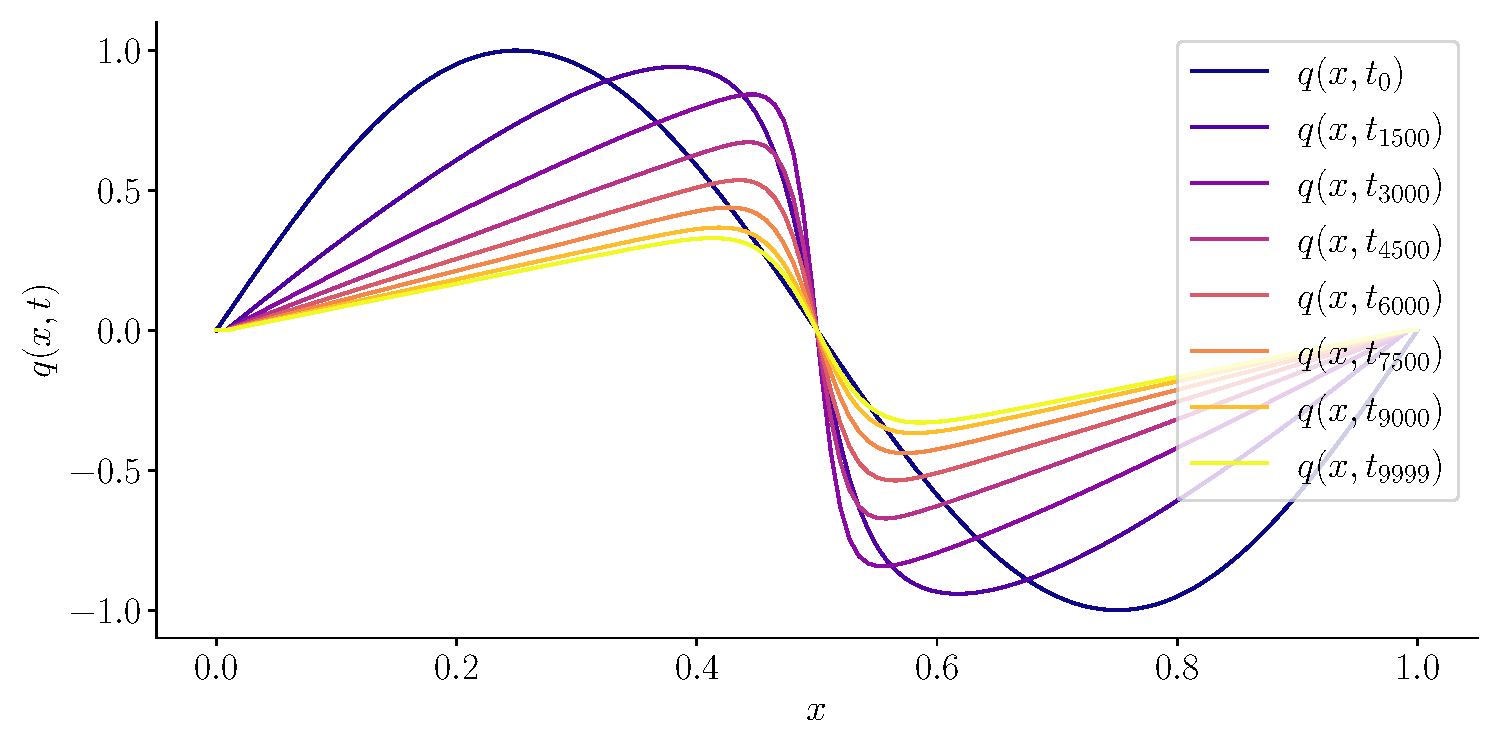
\includegraphics[width=0.8\textwidth]{figures/burgers_evol_001.pdf}
    \caption{Profiles \(q(x,t_k)\) at selected times \(t_k\).}
    \label{fig:burgers-surface}
  \end{subfigure}
  \\[1em]
  \begin{subfigure}[t]{0.56\textwidth}
    \centering
    \hspace{-1.5cm}
    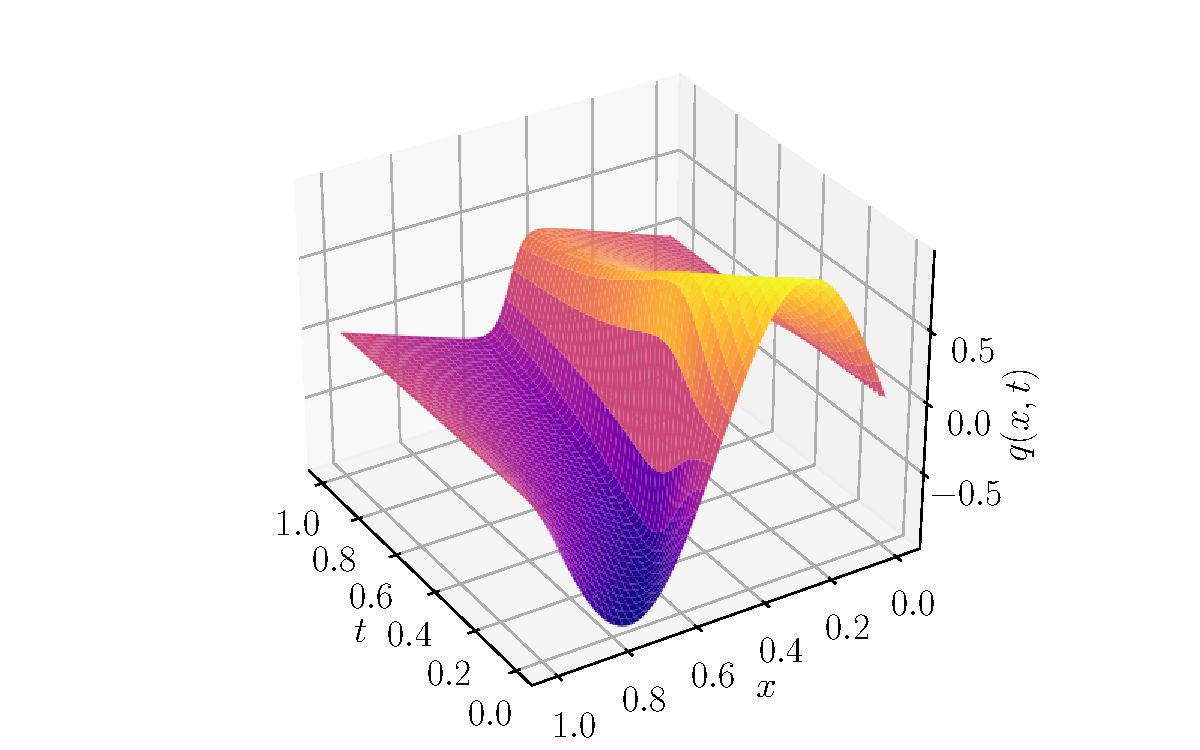
\includegraphics[width=\textwidth]{figures/burgers_sol_001.pdf}
    \caption{3D surface of \(q(x,t)\) for \(\nu=0.01\).}
    \label{fig:burgers-slices}
  \end{subfigure}
  \hspace{-1.5cm}
  \begin{subfigure}[t]{0.5\textwidth}
    \centering
    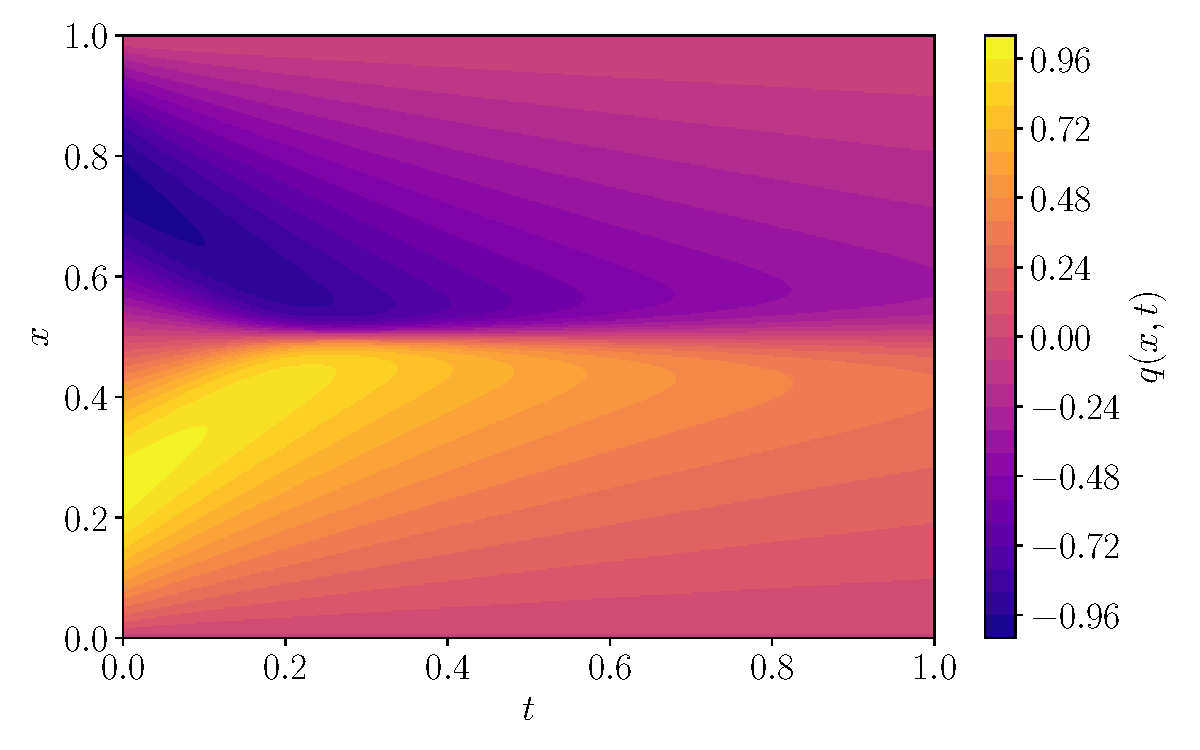
\includegraphics[width=\textwidth]{figures/heatmap_001.pdf}
    \caption{Space–time contour of \(q(x,t)\).}
    \label{fig:burgers-contour}
  \end{subfigure}
  \caption{Dynamics of the viscous Burgers’ equation used for data generation.}
  \label{fig:burgers-data}
\end{figure}
For the Burgers’ dataset, Algorithm~\ref{algorithm_2} is trained on the time interval $t\in[0,0.5]$ and then used to predict over $t\in[0.5,1.0]$. We systematically reduce the number of snapshots to 100\% (10~000 points), 10\% (1~000 points), 1\% (100 points), and 0.2\% (20 points) of the original temporal grid. In each scenario, we estimate OpInf parameters with both second-order (\texttt{'ord2'}) and sixth-order (\texttt{'ord6'}) finite differences, applying an $L^2$-regularization weight $\xi=10^{-2}$.  

Figure~\ref{fig:five_by_two} displays, for each sampling level, the true reduced states $\hat{\mathbf{q}}_{\mathrm{true}}$ (solid) versus the predicted trajectories $\hat{\mathbf{q}}_{\mathrm{pred}}$ (dashed) for both the OpInf and adjoint-trained models. Even at extreme sampling sparsity, the adjoint method produces predictions that are visually indistinguishable from those of OpInf, demonstrating its resilience in the absence of noise.

\newpage

%%%%%%%%%%%%%%%%%%%%%%%%%%%%%%%%% DATA DENSITY REDUCTION  - BURGERS %%%%%%%%%%%%%%%%%%%%%%%%%%%%%%%%%

\subsection*{Data Density Reduction}

\vspace{1.0cm}

\begin{figure}[h!]
  \centering
  \begin{subfigure}[c]{0.49\textwidth}
      \centering
      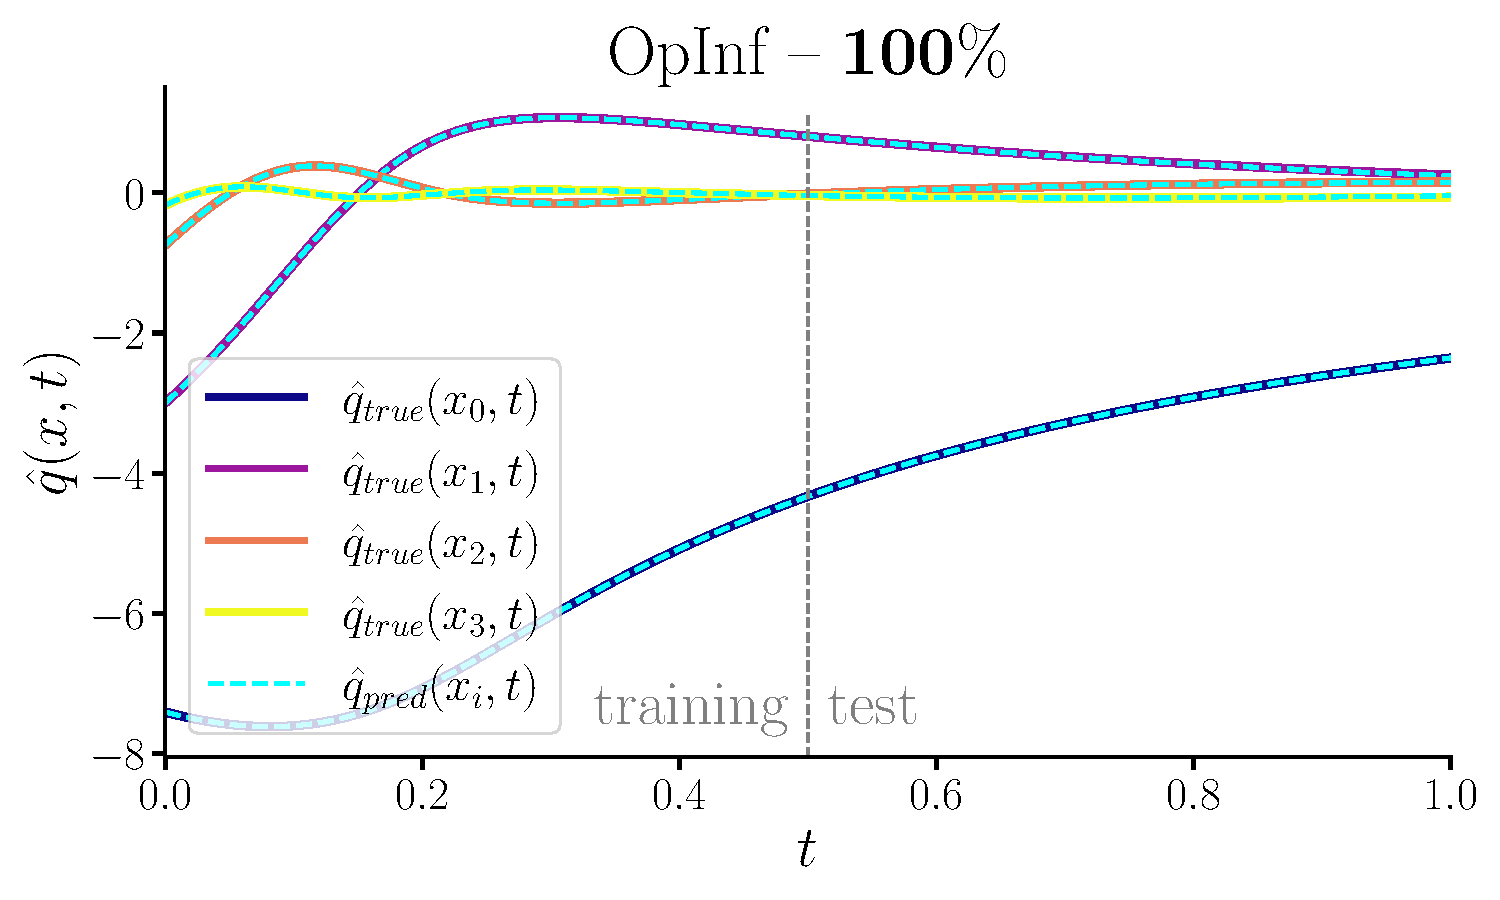
\includegraphics[width=\linewidth]{rom_data_density_100_OpInf.pdf}
  \end{subfigure}
  \begin{subfigure}[c]{0.49\textwidth}
      \centering
      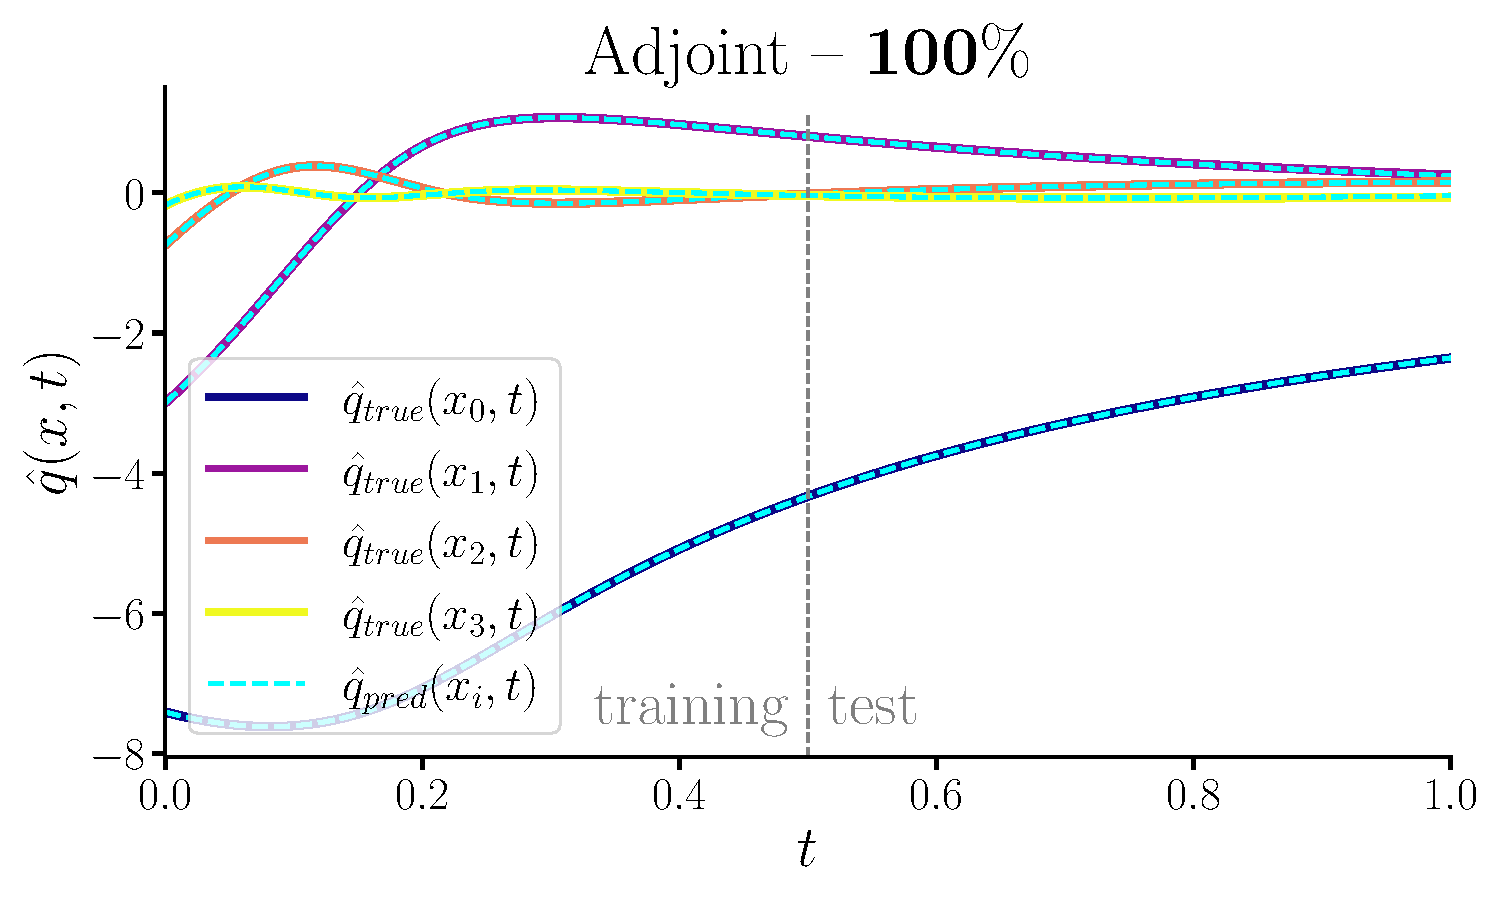
\includegraphics[width=\linewidth]{rom_data_density_100_Adj.pdf}
  \end{subfigure} \\[1ex]
    
  \begin{subfigure}[c]{0.49\textwidth}
      \centering
      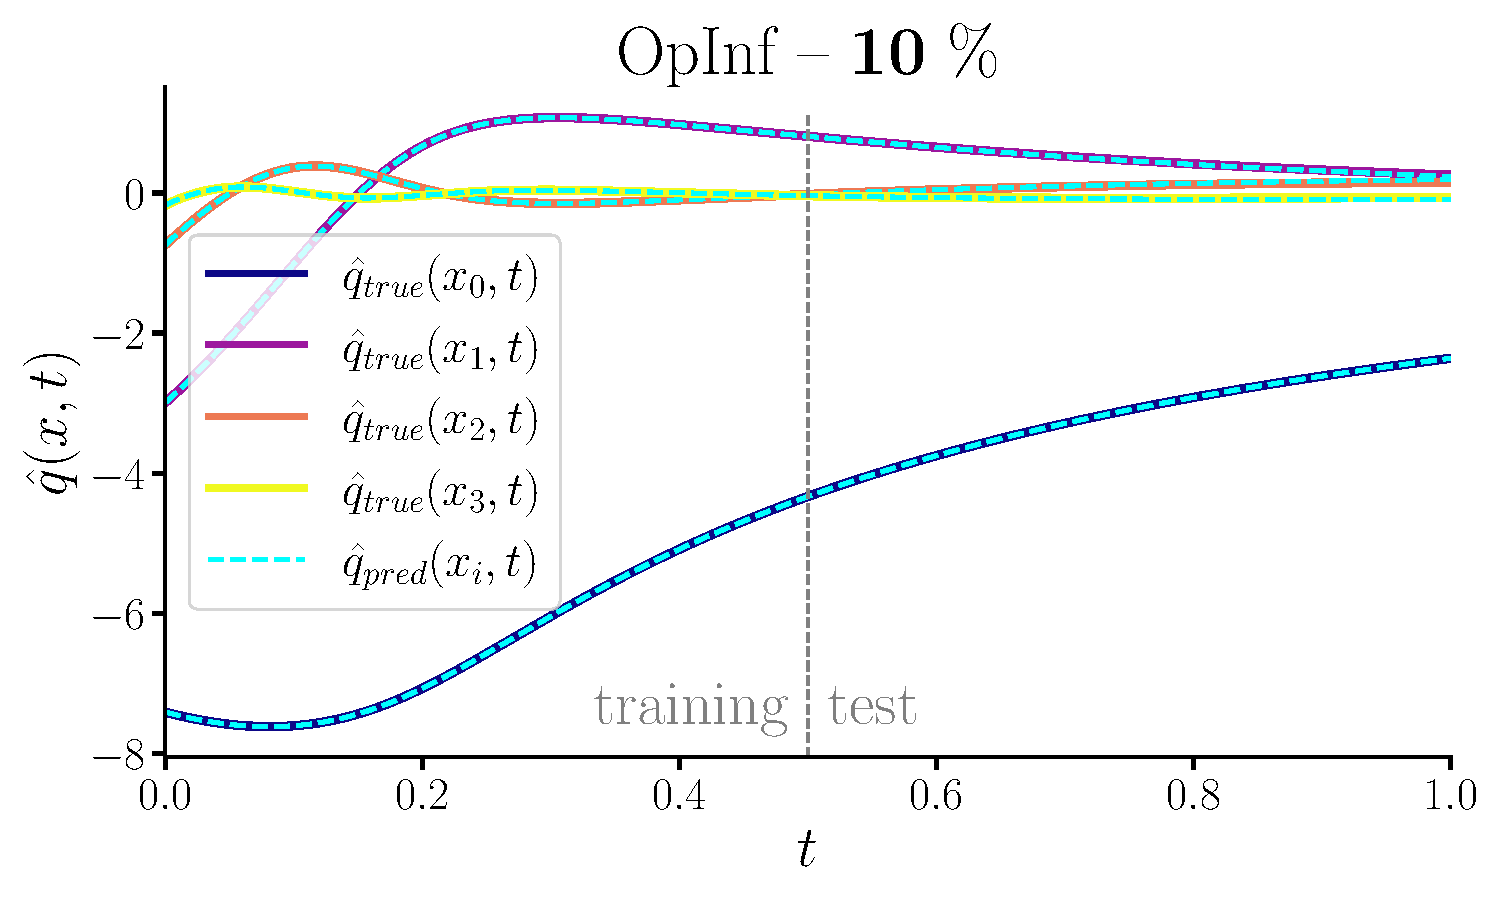
\includegraphics[width=\linewidth]{rom_data_density_10_OpInf.pdf}
  \end{subfigure} 
  \begin{subfigure}[c]{0.49\textwidth}
      \centering
      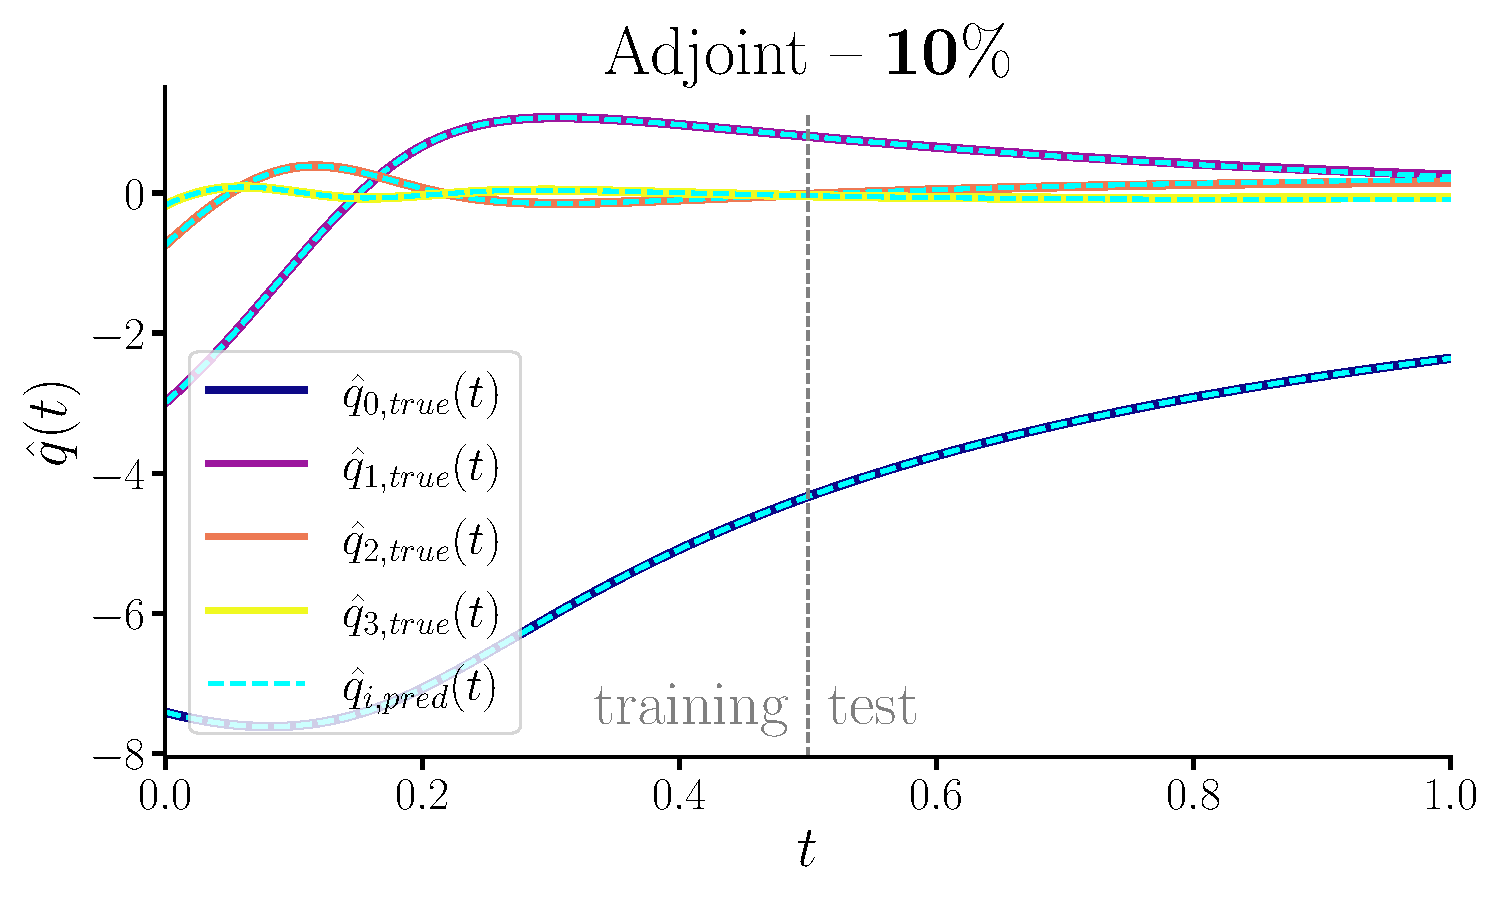
\includegraphics[width=\linewidth]{figures/rom_data_density_10_Adj.pdf}
  \end{subfigure} \\[1ex]
    
  \begin{subfigure}[c]{0.49\textwidth}
      \centering
      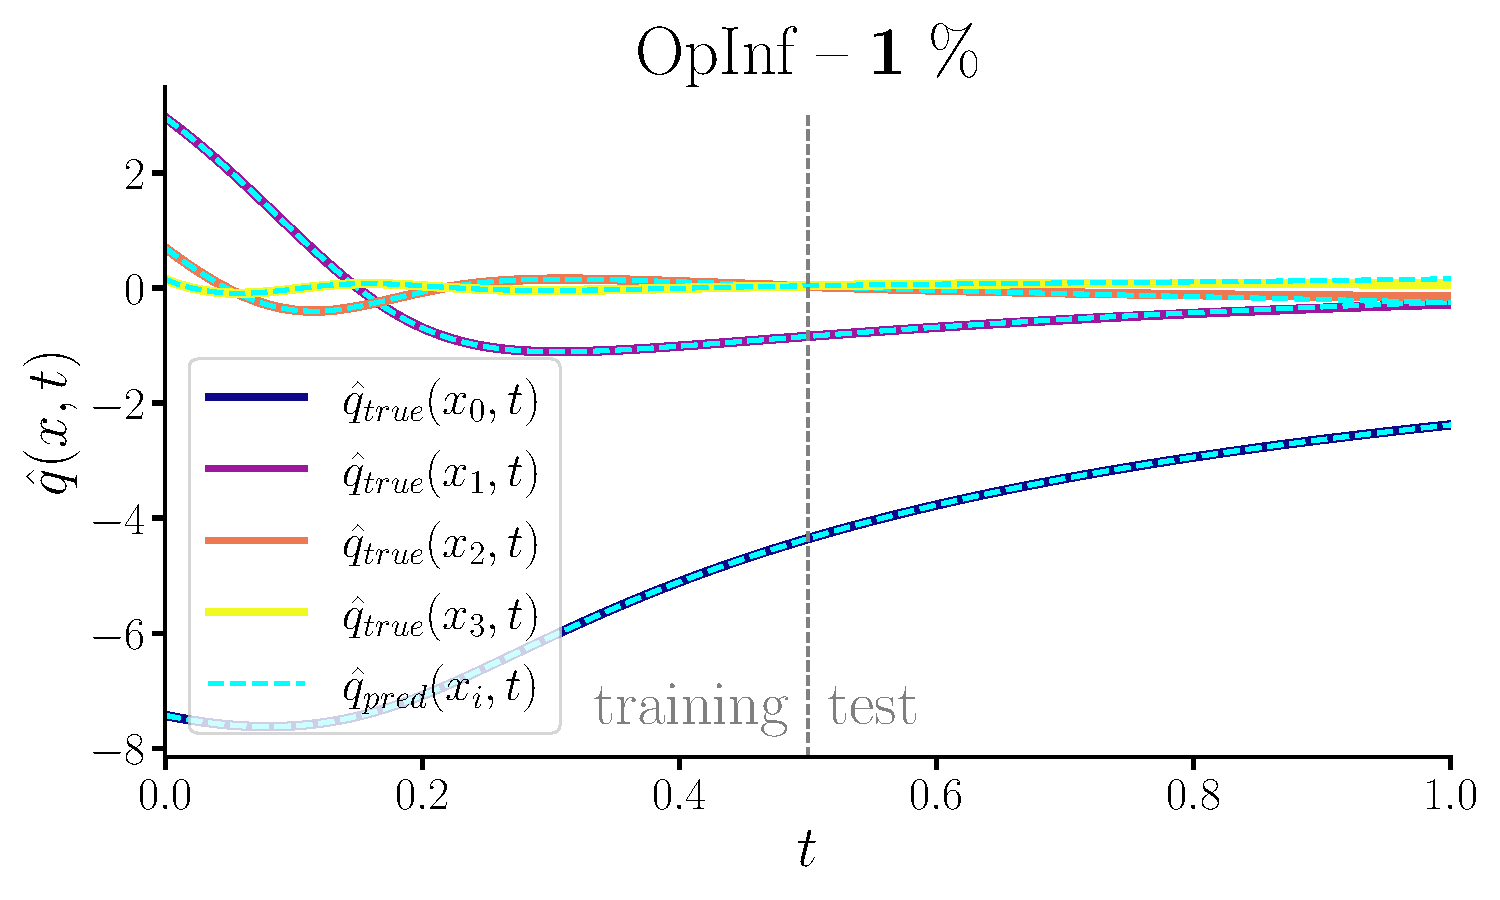
\includegraphics[width=\linewidth]{rom_data_density_1_OpInf.pdf}
  \end{subfigure} 
  \begin{subfigure}[c]{0.49\textwidth}
      \centering
      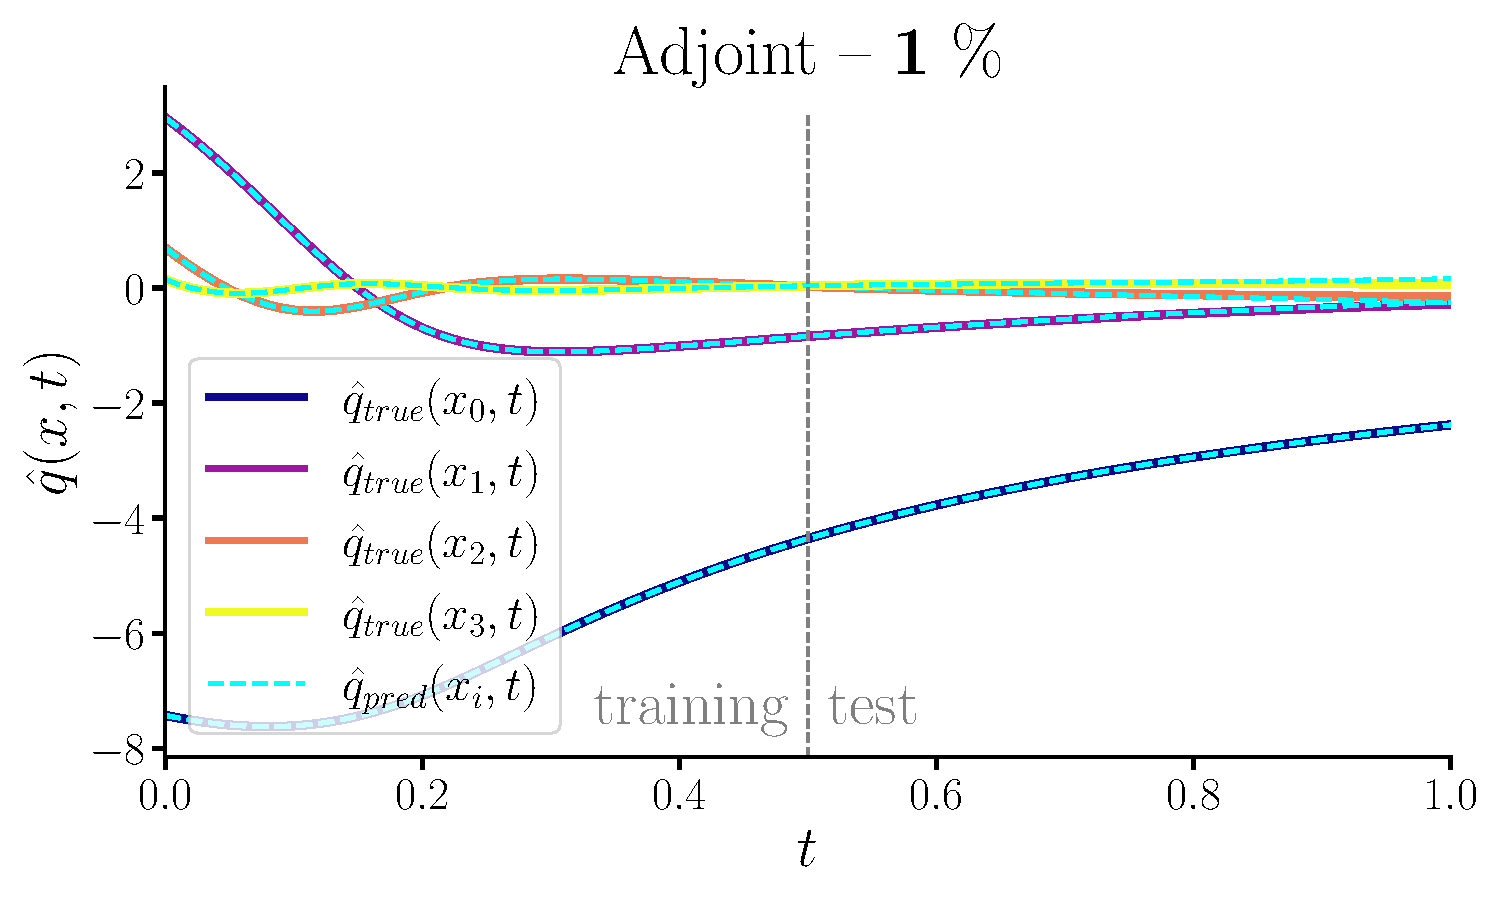
\includegraphics[width=\linewidth]{rom_data_density_1_Adj.pdf}
  \end{subfigure} \\[1ex]
    
  \begin{subfigure}[c]{0.49\textwidth}
      \centering
      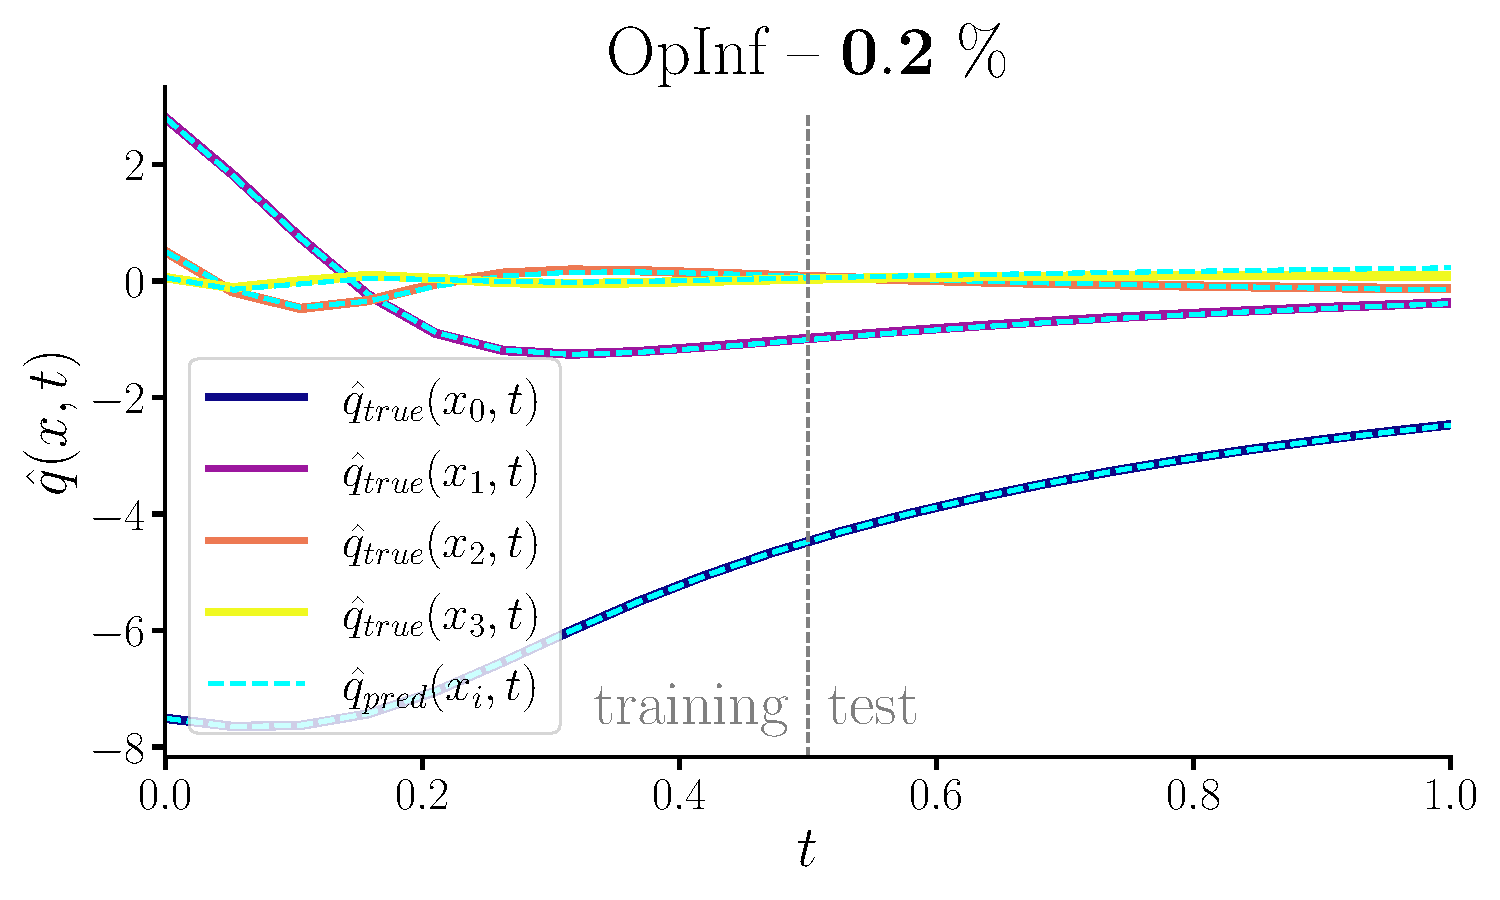
\includegraphics[width=\linewidth]{rom_data_density_02_OpInf.pdf}
  \end{subfigure} 
  \begin{subfigure}[c]{0.49\textwidth}
      \centering
      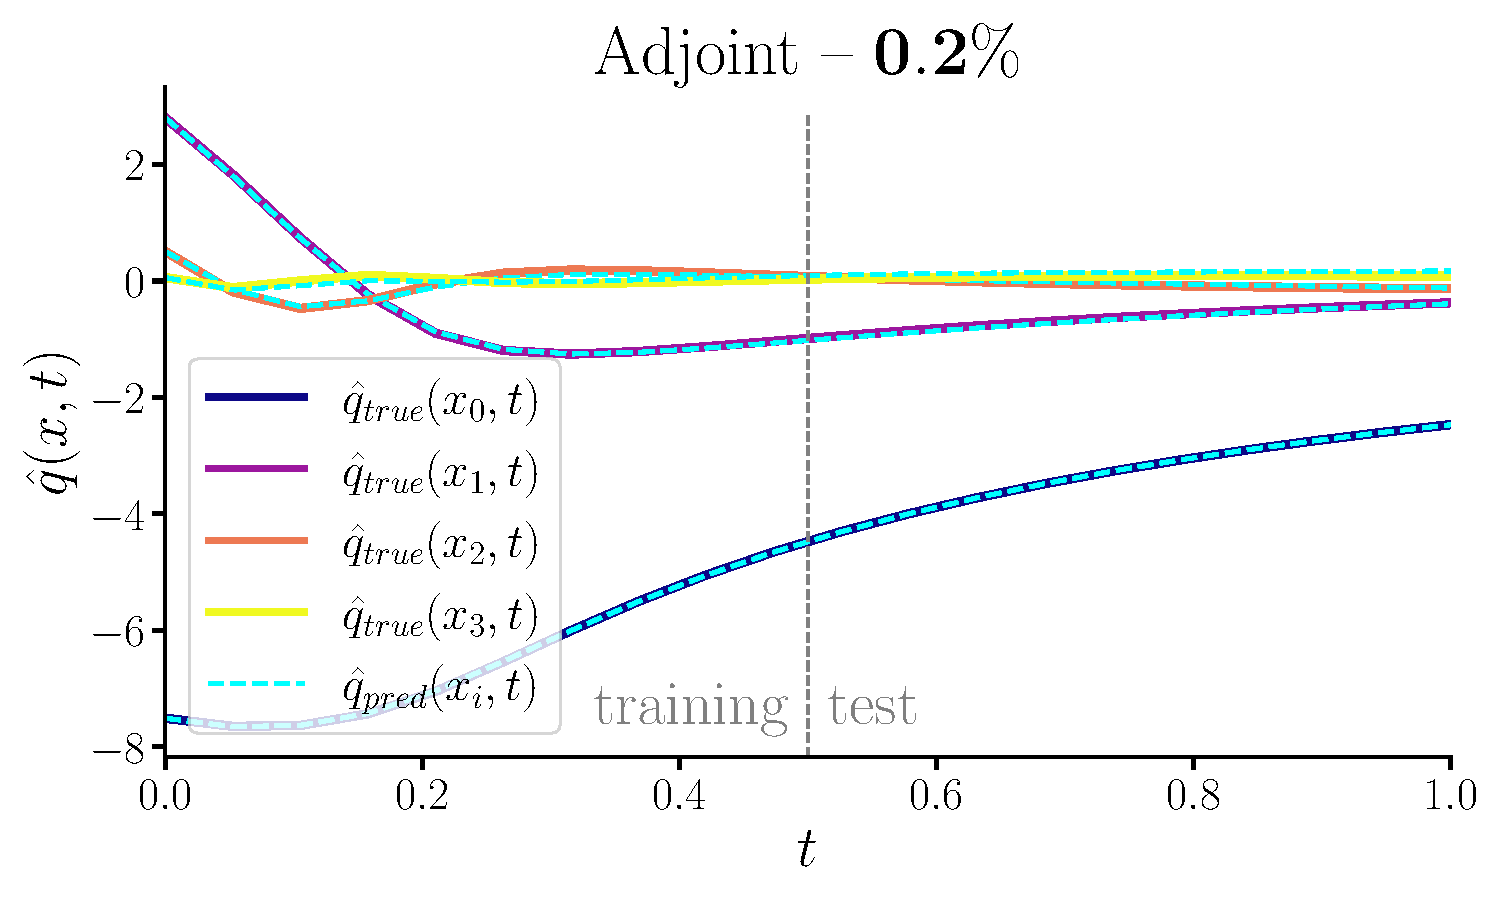
\includegraphics[width=\linewidth]{rom_data_density_02_Adj.pdf}
  \end{subfigure} \\[1ex]
  \caption{Data density reduction results for the Burgers' Equation synthetic experiment.}
  \label{fig:five_by_two}
\end{figure}

\newpage

%%%%%% Prediction Error vs. Time (data density - Burgers) %%%%%%

To quantify the impact of training data sparsity, we compute the prediction error in the test region $t\in[0.5,1]$ for each sampling density. Specifically, we solve the ROM-OpInf initial value problem with the learned operators and compare the trajectories against the true reduced states for each sampling level (100\%, 10\%, 1\%, 0.2\% respectively):\\
  $$\|\hat{\mathbf{q}}_{\mathrm{true}}(t) - \hat{\mathbf{q}}_{\mathrm{pred}}(t)\|_2,
  \quad t\in[0.5,1].$$
Figure~\ref{fig:twobytwo} compares the OpInf and adjoint error curves across all sampling levels. The adjoint method produces errors similar to or even lower than when the sixth-order stencil is used, confirming its accuracy capturing time-derivative information under limited data.

\vspace{0.7cm}

\begin{figure}[h!]
  \centering
  
  % First row of subfigures
  \begin{subfigure}[b]{0.48\textwidth}
    \centering
    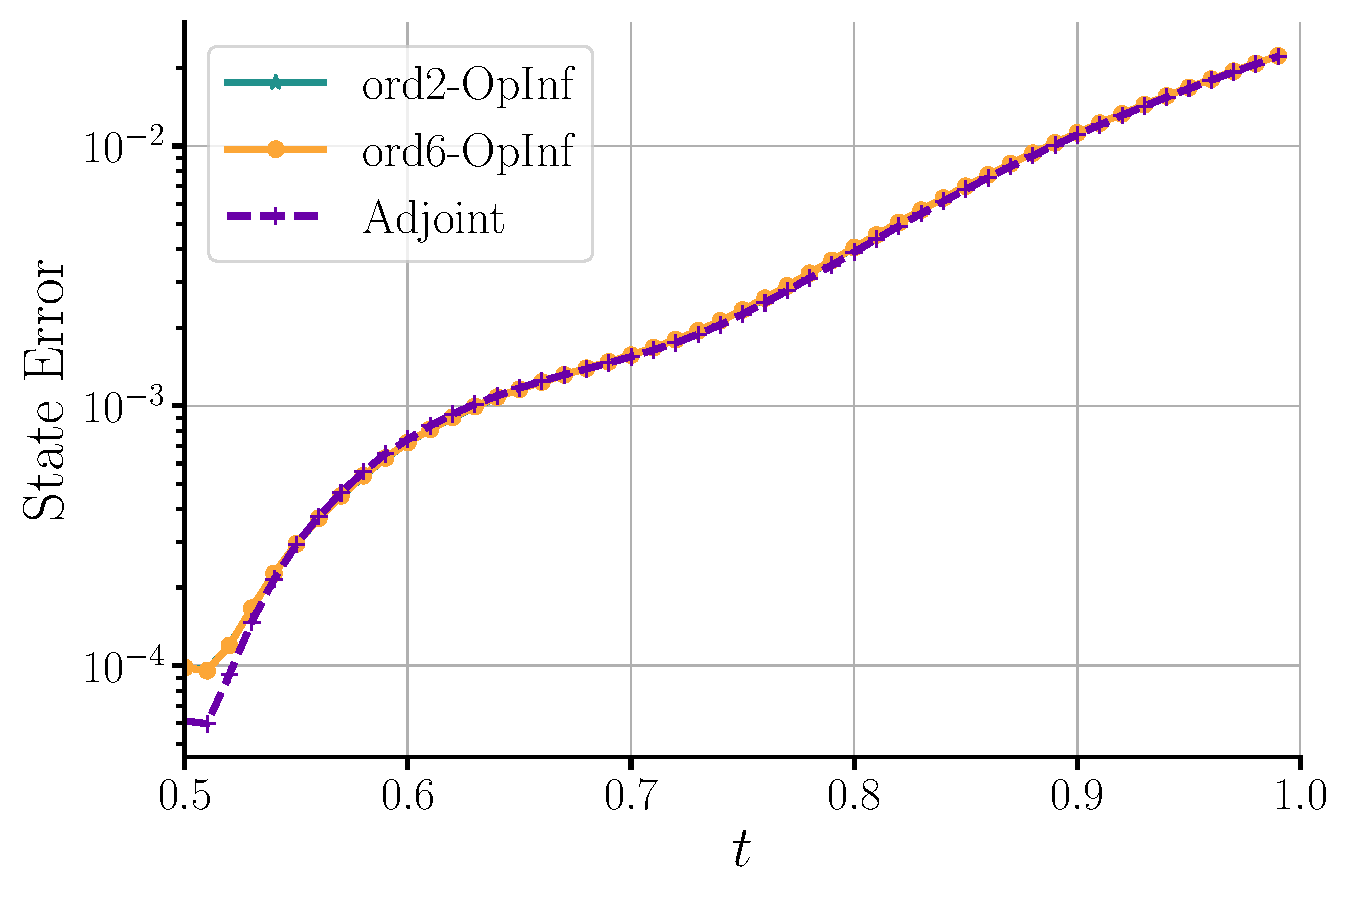
\includegraphics[width=\linewidth]{pred_error_vs_time_data_density_100.pdf}
    \caption{100\% of the data.}
    \label{fig:image1}
  \end{subfigure}
  \quad
  \begin{subfigure}[b]{0.48\textwidth}
    \centering
    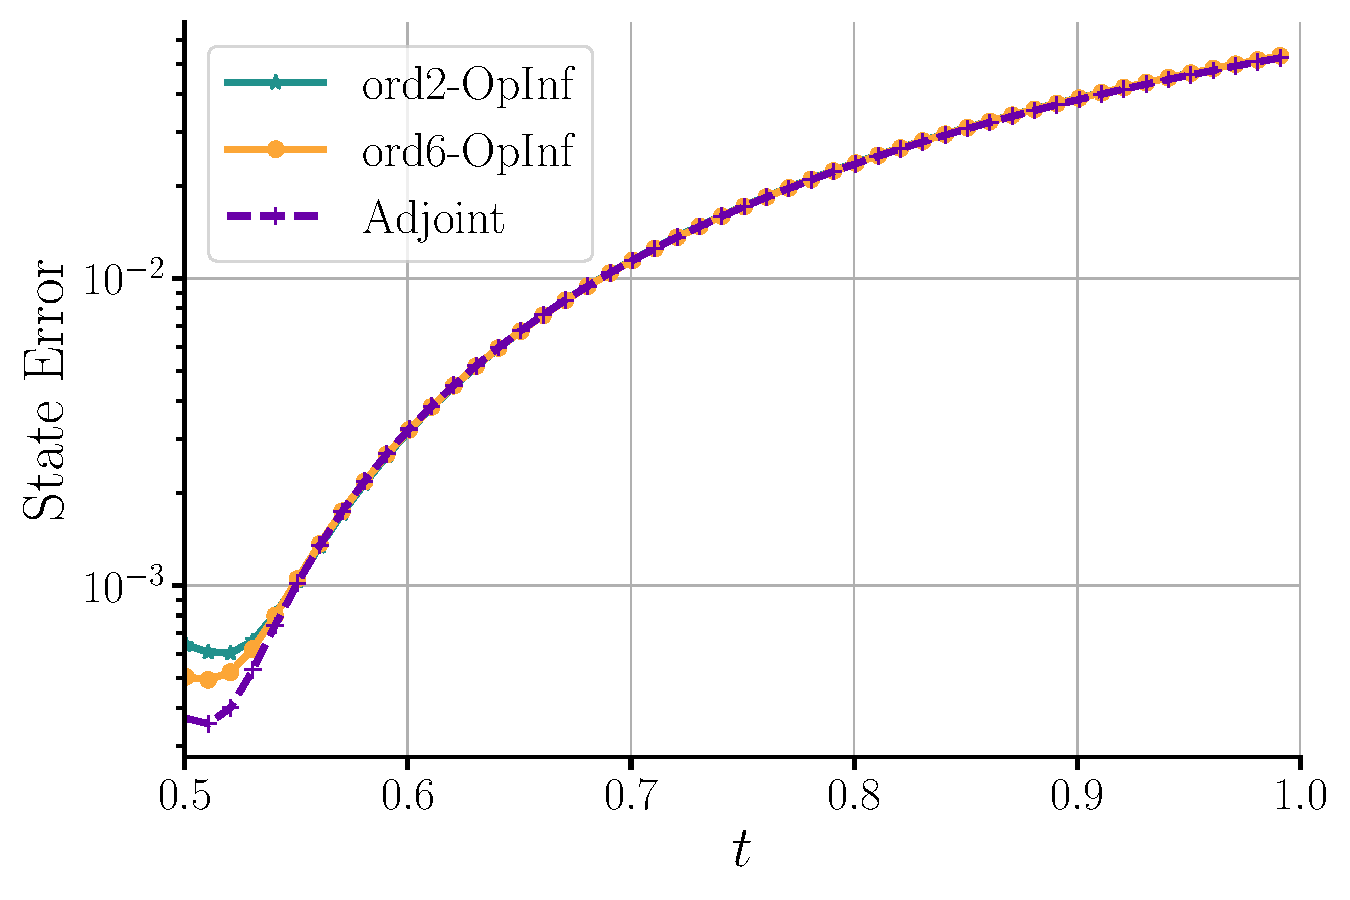
\includegraphics[width=\linewidth]{pred_error_vs_time_data_density_10.pdf}
    \caption{10\% of the data.}
    \label{fig:image2}
  \end{subfigure}
  
  \vskip\baselineskip
  
  % Second row of subfigures
  \begin{subfigure}[b]{0.48\textwidth}
    \centering
    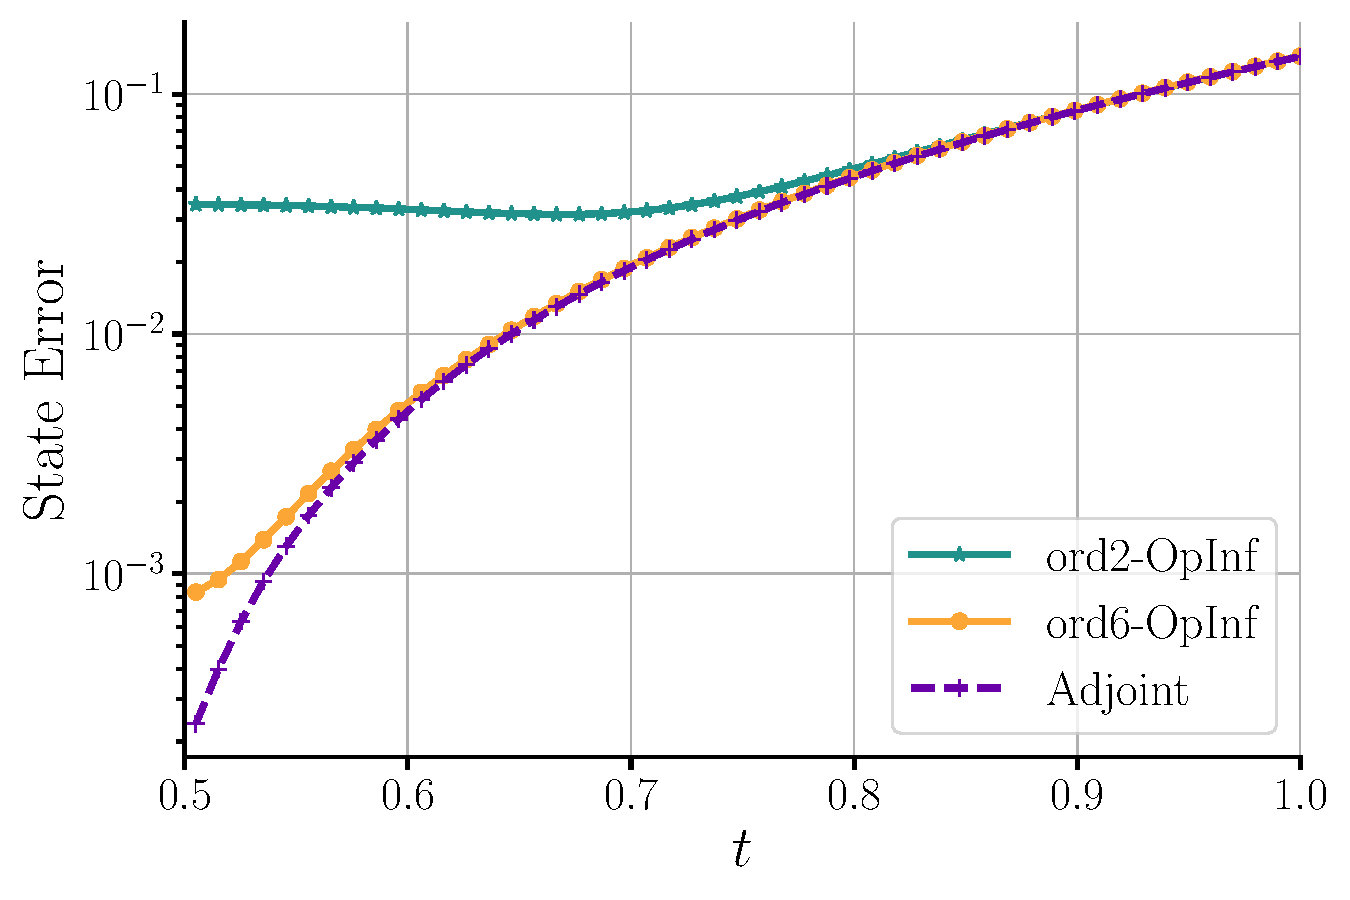
\includegraphics[width=\linewidth]{pred_error_vs_time_data_density_1.pdf}
    \caption{1\% of the data.}
    \label{fig:image3}
  \end{subfigure}
  \quad
  \begin{subfigure}[b]{0.48\textwidth}
    \centering
    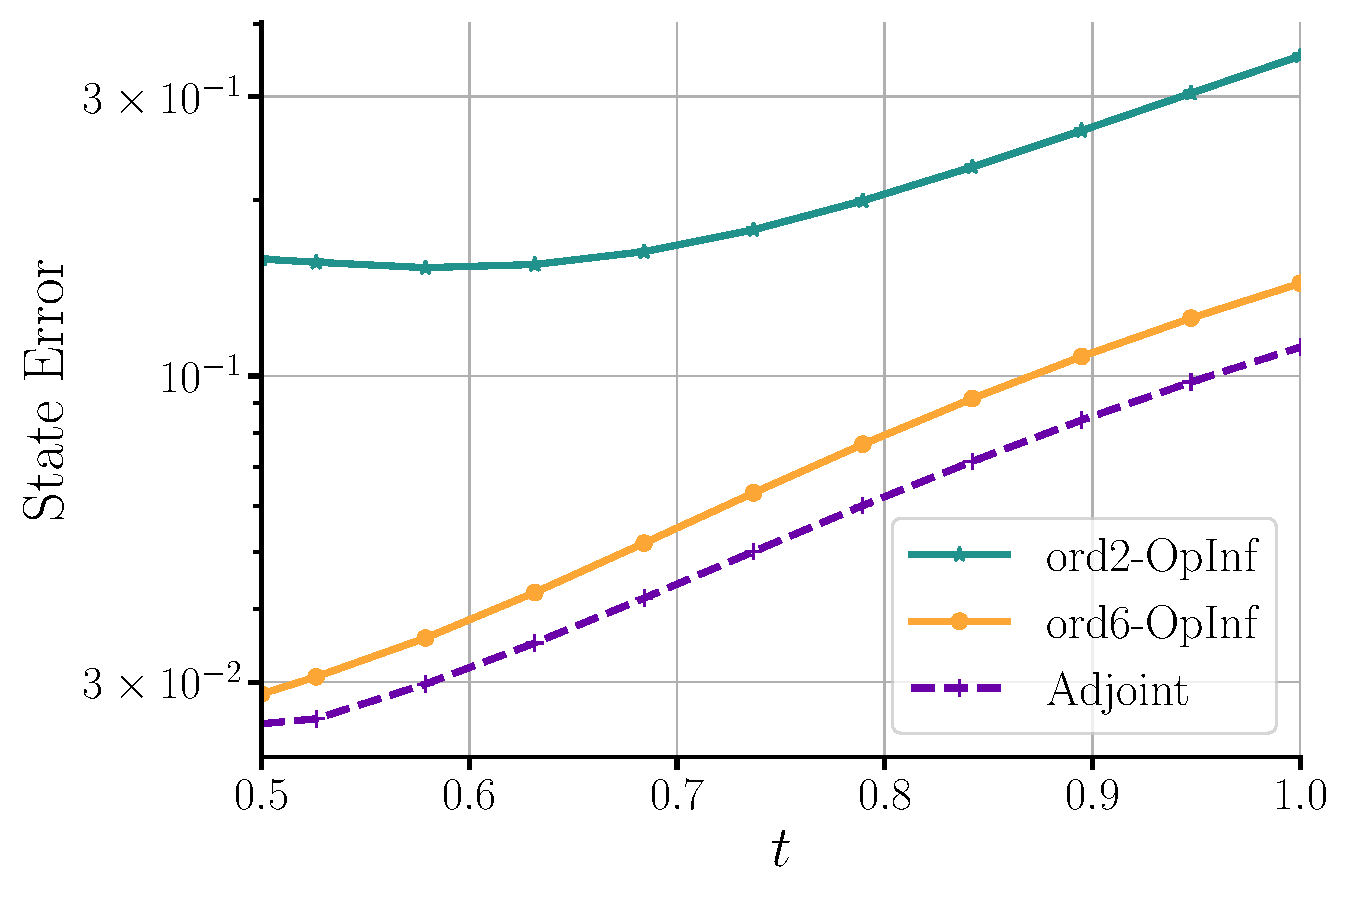
\includegraphics[width=\linewidth]{pred_error_vs_time_data_density_02.pdf}
    \caption{0.2\% of the data.}
    \label{fig:image4}
  \end{subfigure}
  
  \caption{Prediction error vs. time for each data density reduction run in the Burgers' Equation experiment.}
  \label{fig:twobytwo}
\end{figure}

\newpage

%%%%%% Relative Error vs. Time (data density - Burgers) %%%%%%

Figure~\ref{fig:twobytwo2} shows the relative error\\
$$\frac{\|\hat{\mathbf{q}}_{\mathrm{true}}(t) - \hat{\mathbf{q}}_{\mathrm{pred}}(t)\|_2}
       {\|\hat{\mathbf{q}}_{\mathrm{true}}(t)\|_2},
  \quad t\in[0,1],$$
as a function of the ROM dimension $r$. Again, each subplot corresponds to one of the four sampling densities. Both methods exhibit the expected decay in relative error with increasing $r$. However, in the most extreme sparsity case (0.2\%), the adjoint-trained model achieves marginally lower errors, suggesting it can construct more efficient reduced bases when snapshot information is scarce.

\vspace{0.7cm}

\begin{figure}[h!]
  \centering
  
  % First row of subfigures
  \begin{subfigure}[b]{0.48\textwidth}
    \centering
    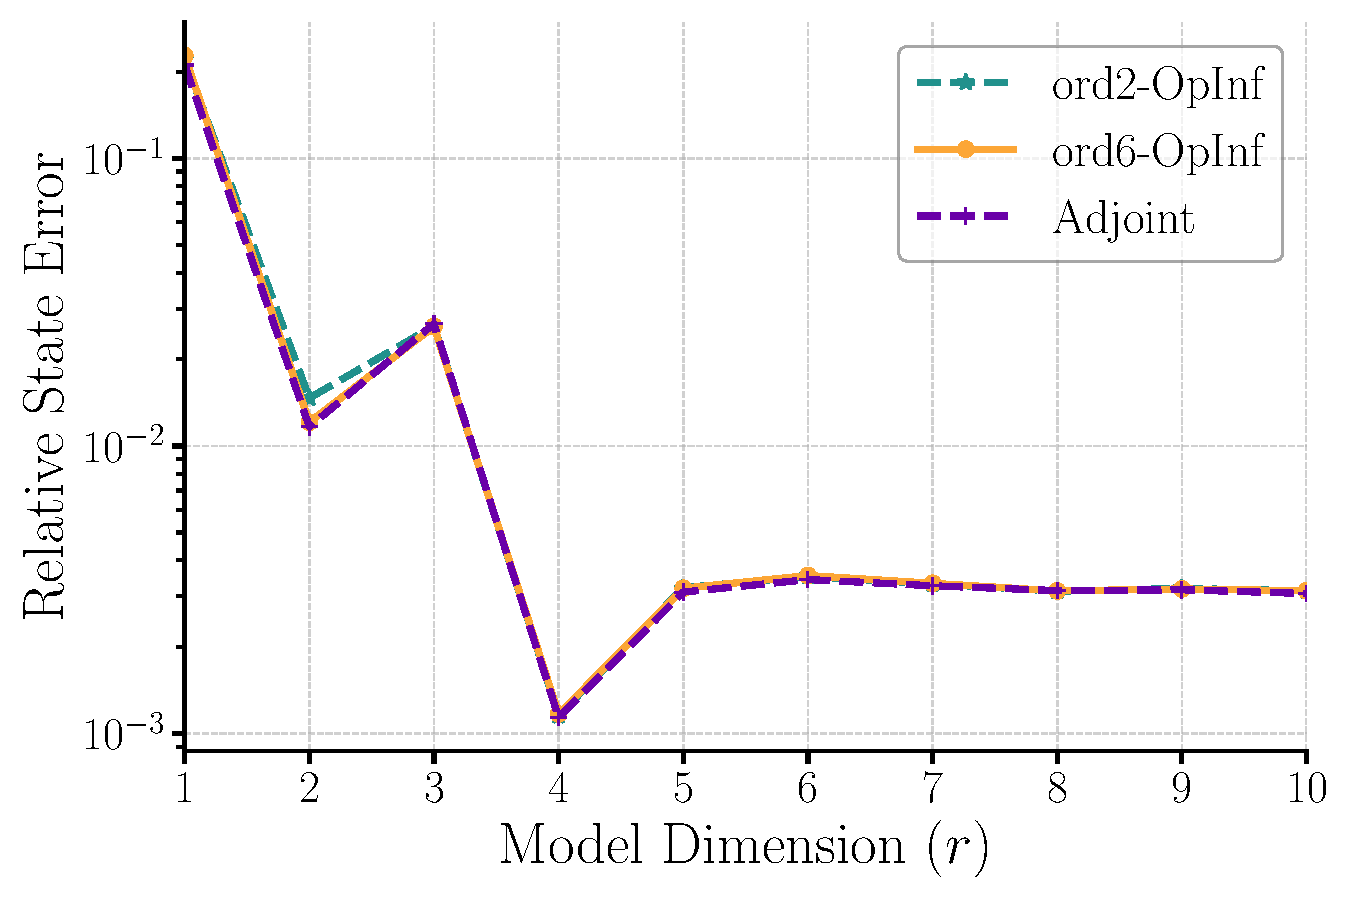
\includegraphics[width=\linewidth]{rel_error_vs_r_data_density_100.pdf}
    \caption{100\% of the data.}
    \label{fig:image1}
  \end{subfigure}
  \quad
  \begin{subfigure}[b]{0.48\textwidth}
    \centering
    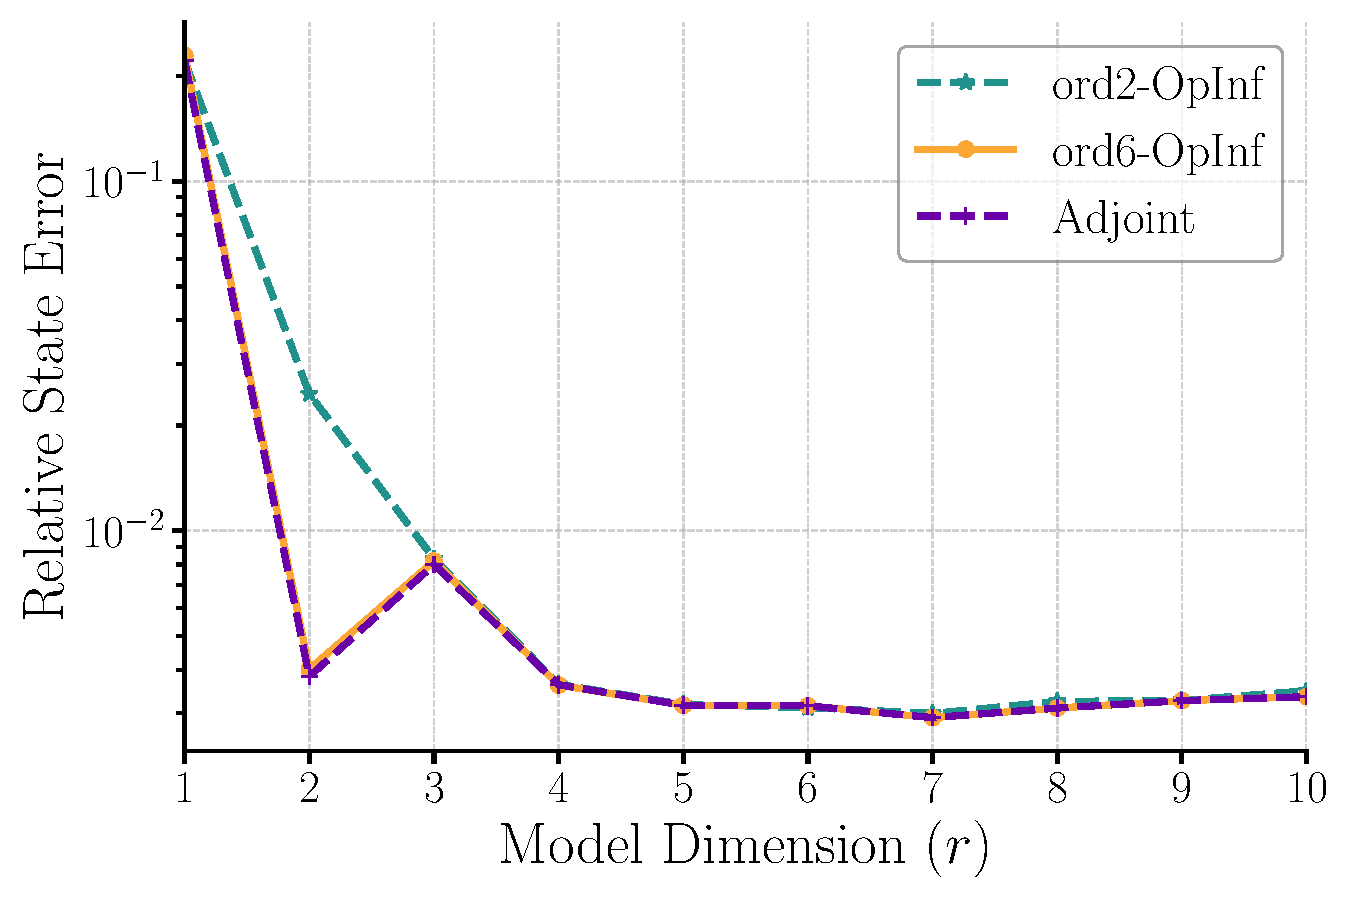
\includegraphics[width=\linewidth]{rel_error_vs_r_data_density_10.pdf}
    \caption{10\% of the data.}
    \label{fig:image2}
  \end{subfigure}
  
  \vskip\baselineskip
  
  % Second row of subfigures
  \begin{subfigure}[b]{0.48\textwidth}
    \centering
    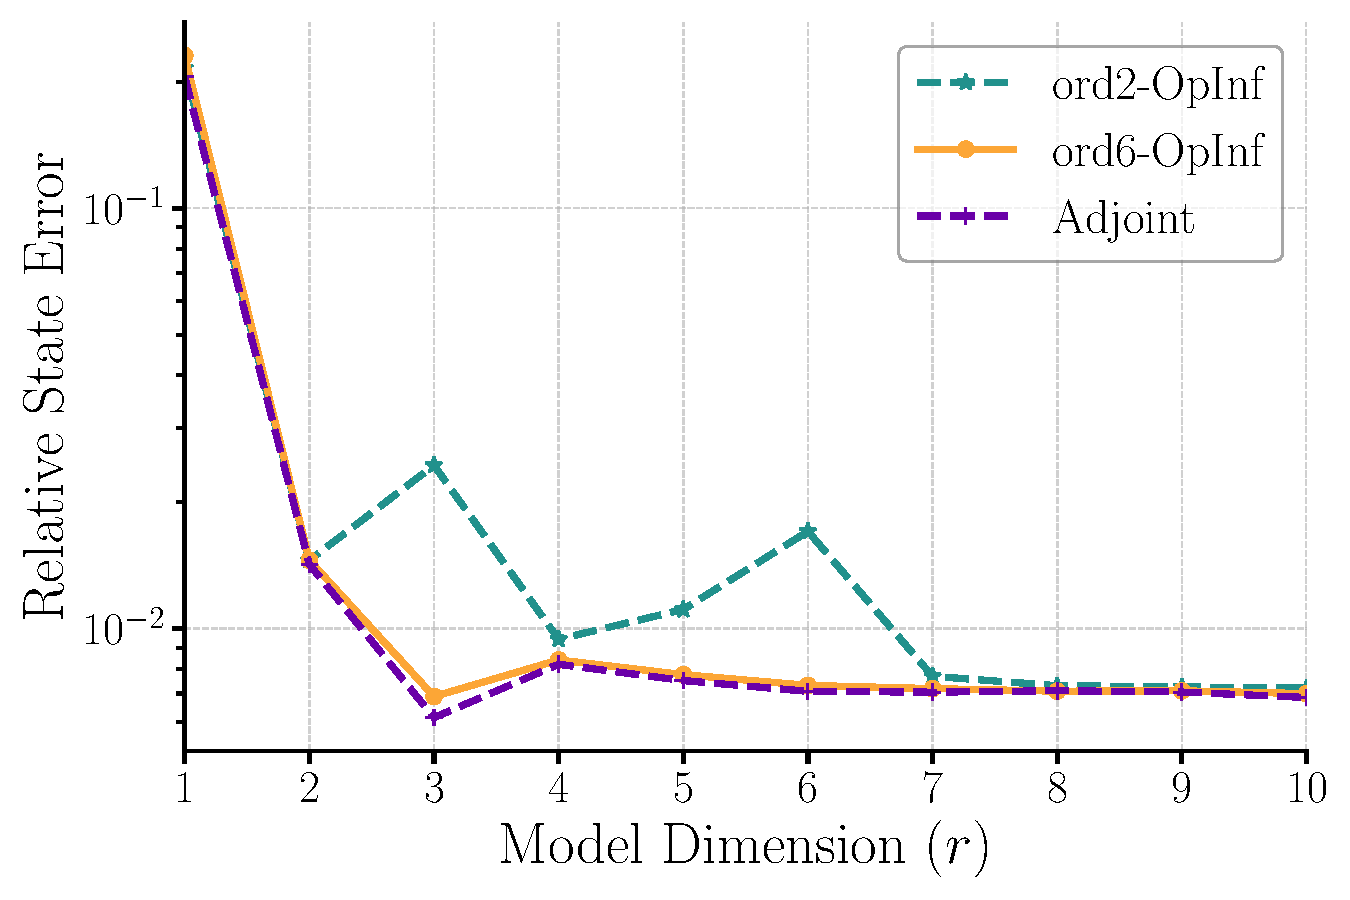
\includegraphics[width=\linewidth]{rel_error_vs_r_data_density_1.pdf}
    \caption{1\% of the data.}
    \label{fig:image3}
  \end{subfigure}
  \quad
  \begin{subfigure}[b]{0.48\textwidth}
    \centering
    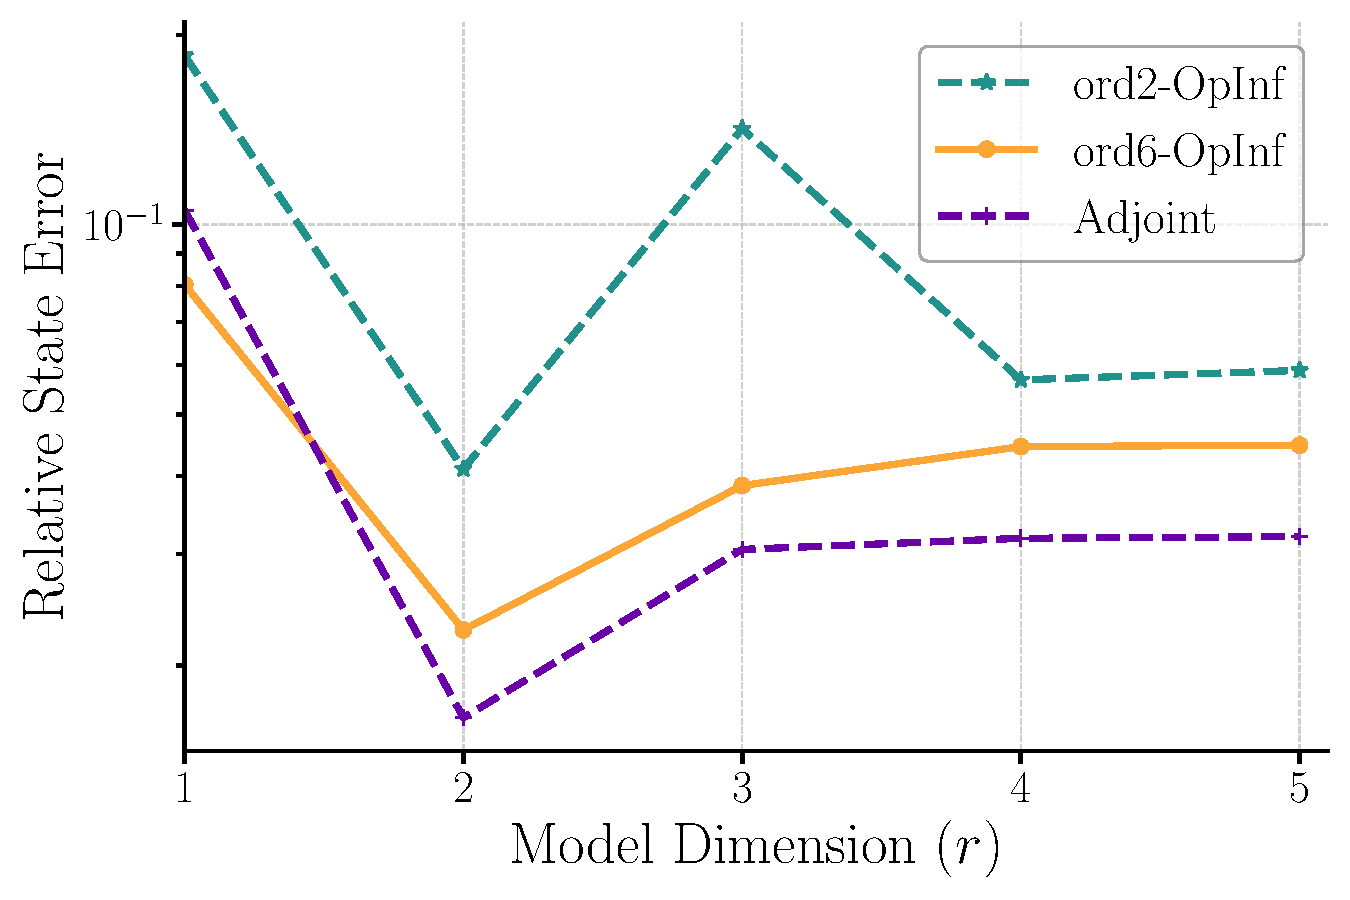
\includegraphics[width=\linewidth]{rel_error_vs_r_data_density_02.pdf}
    \caption{0.2\% of the data.}
    \label{fig:image4}
  \end{subfigure}
  
  \caption{Relative error vs. $r$ for each data density reduction run in the Burgers' Equation experiment.}
  \label{fig:twobytwo2}
\end{figure}

\newpage

%%%%%%%%%%%%%%%%%%%%%%%%%%%%%%%%% NOISE PERTURBATION %%%%%%%%%%%%%%%%%%%%%%%%%%%%%%%%%%

\subsection*{Noise Perturbation}

\vspace{1.0cm}

\begin{figure}[h!]
  \centering
  \begin{subfigure}[c]{0.49\textwidth}
      \centering
      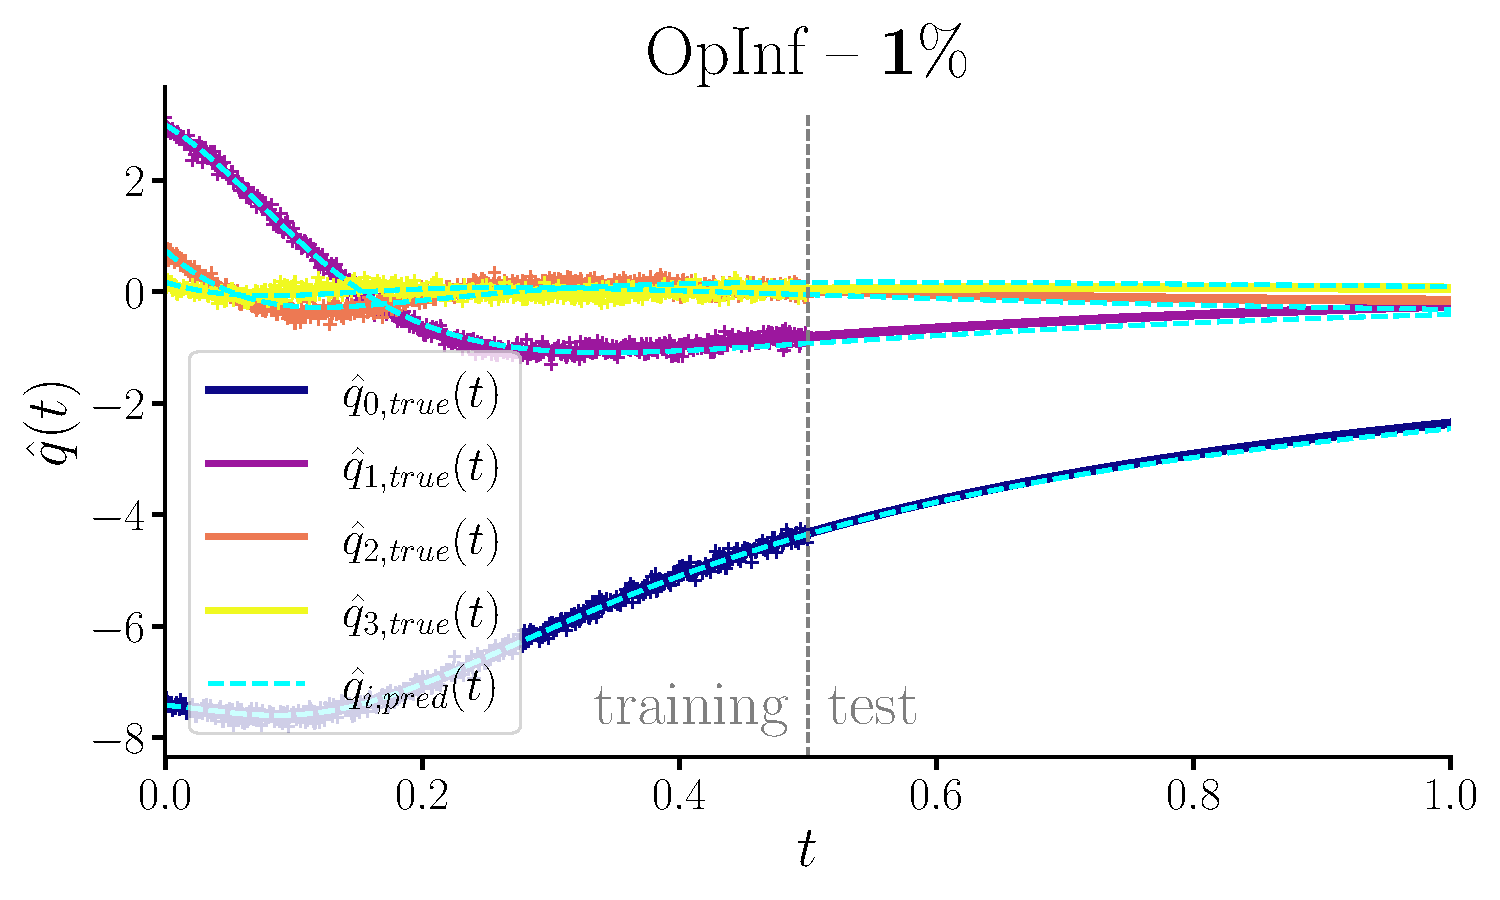
\includegraphics[width=\linewidth]{rom_noise_1_OpInf.pdf}
  \end{subfigure}
  \begin{subfigure}[c]{0.49\textwidth}
      \centering
      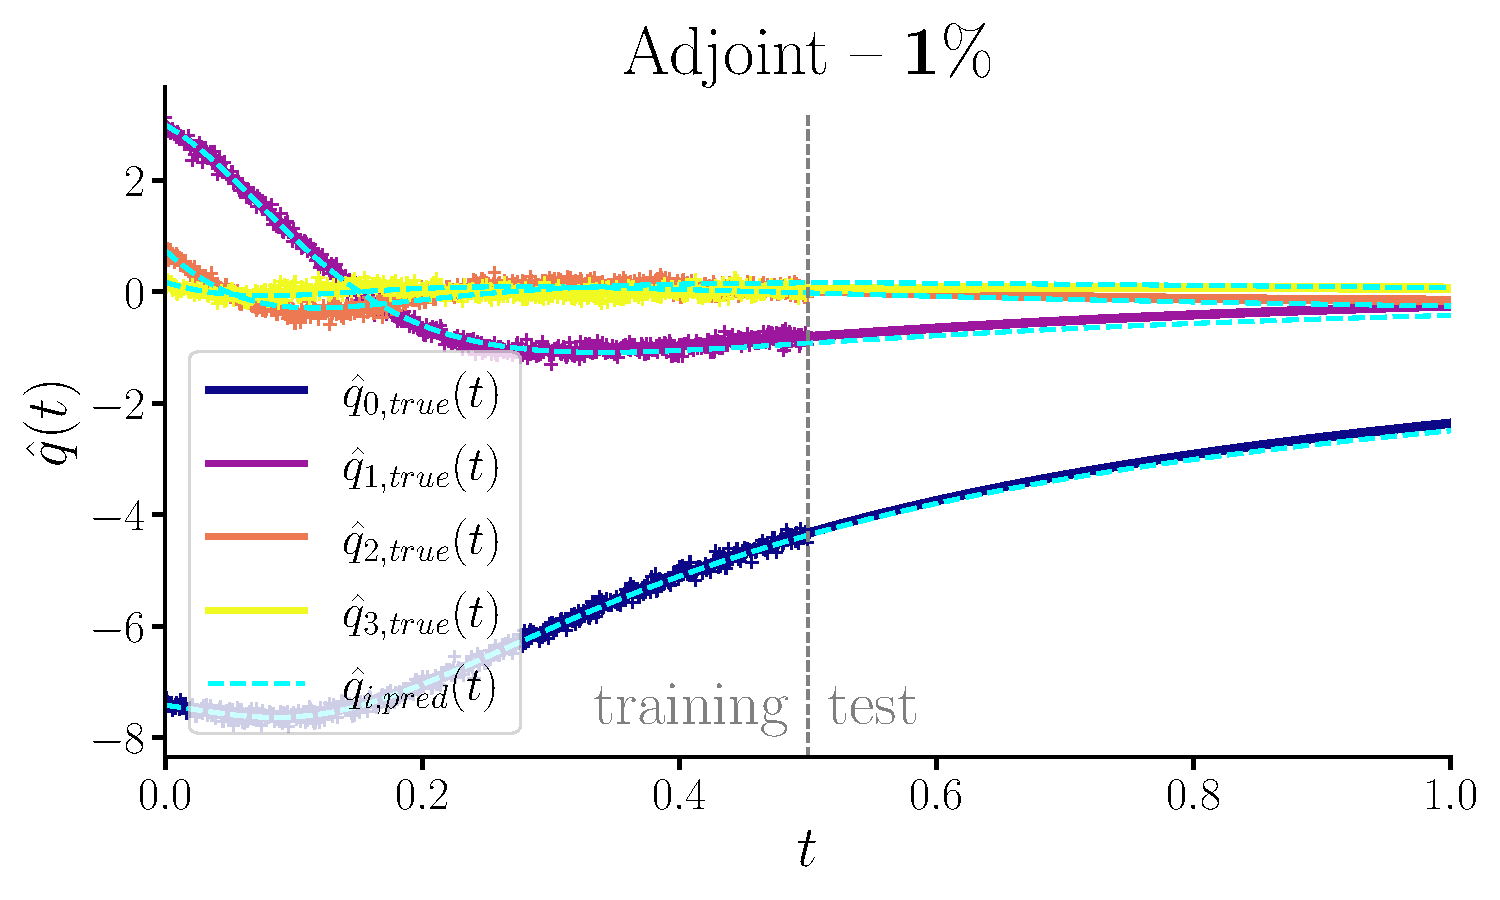
\includegraphics[width=\linewidth]{rom_noise_1_Adj.pdf}
  \end{subfigure} \\[1ex]
    
  \begin{subfigure}[c]{0.49\textwidth}
      \centering
      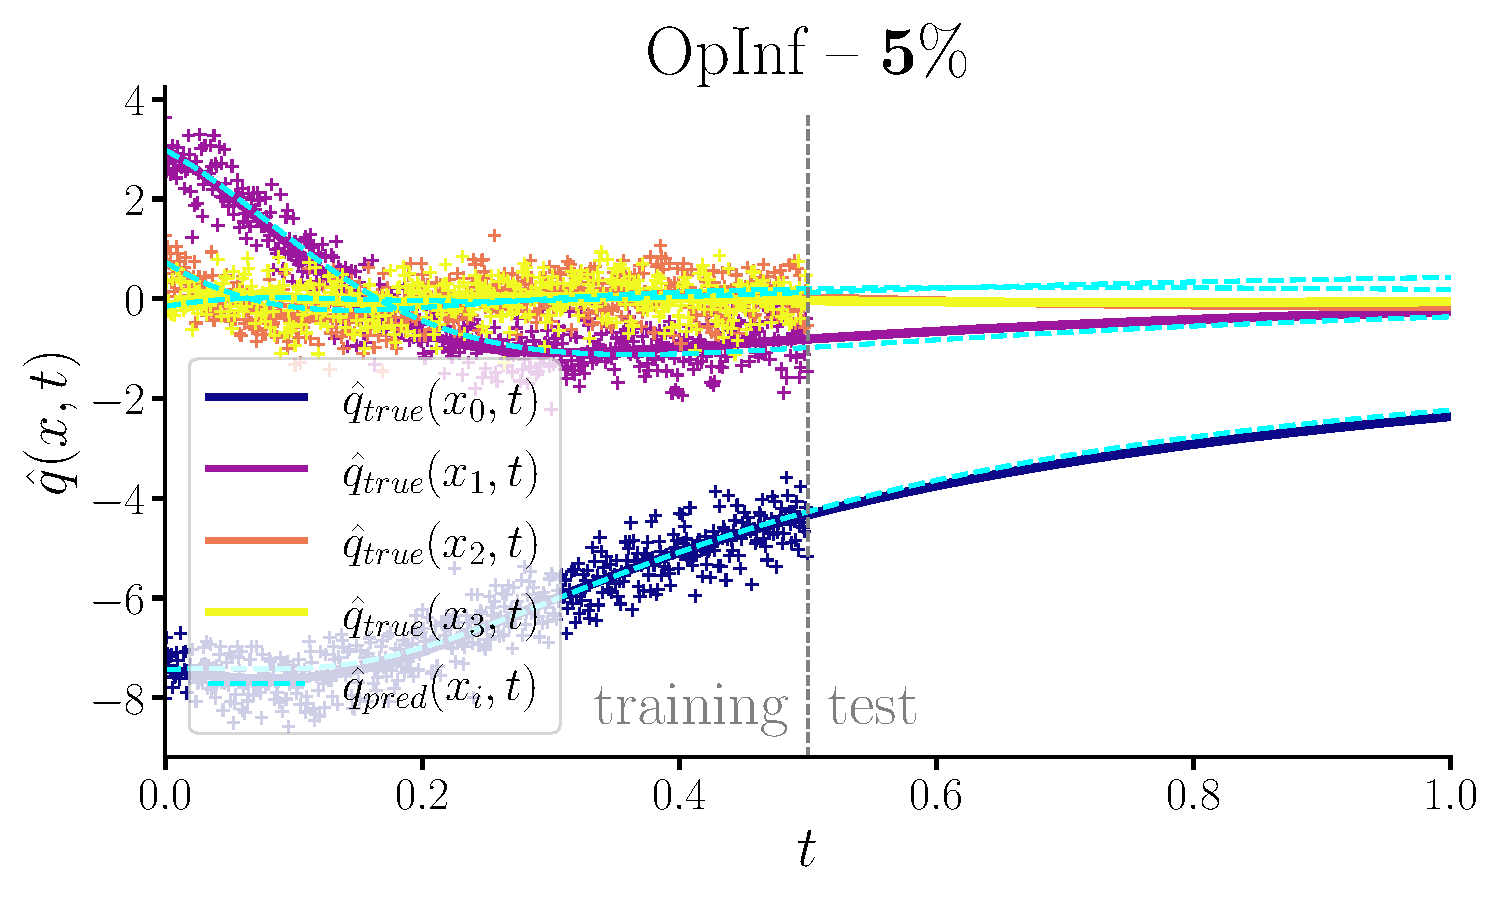
\includegraphics[width=\linewidth]{rom_noise_5_OpInf.pdf}
  \end{subfigure} 
  \begin{subfigure}[c]{0.49\textwidth}
      \centering
      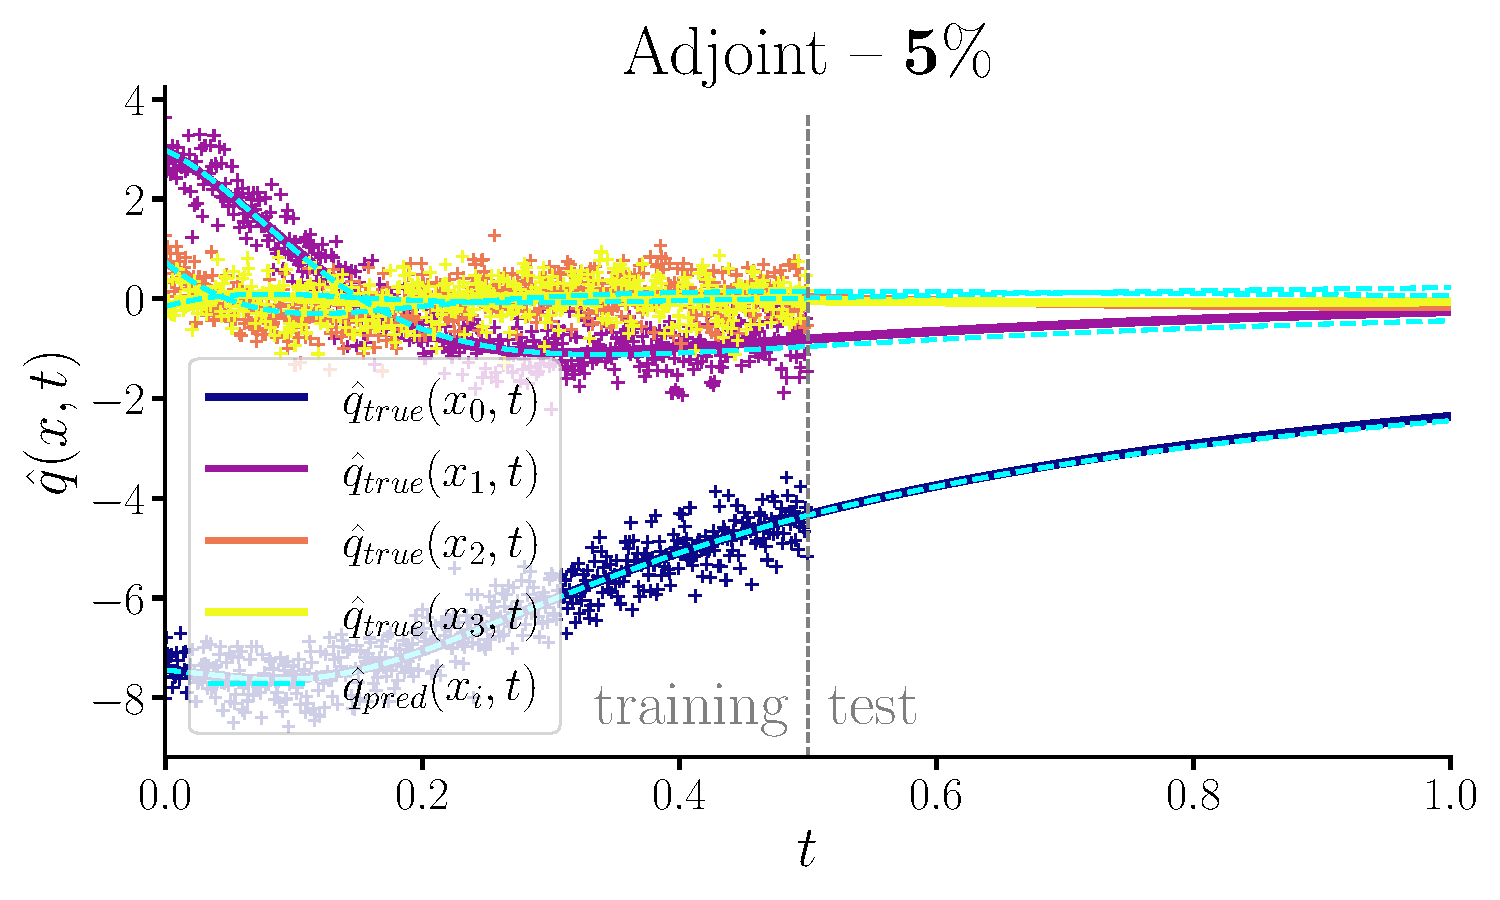
\includegraphics[width=\linewidth]{rom_noise_5_Adj.pdf}
  \end{subfigure} \\[1ex]
    
  \begin{subfigure}[c]{0.49\textwidth}
      \centering
      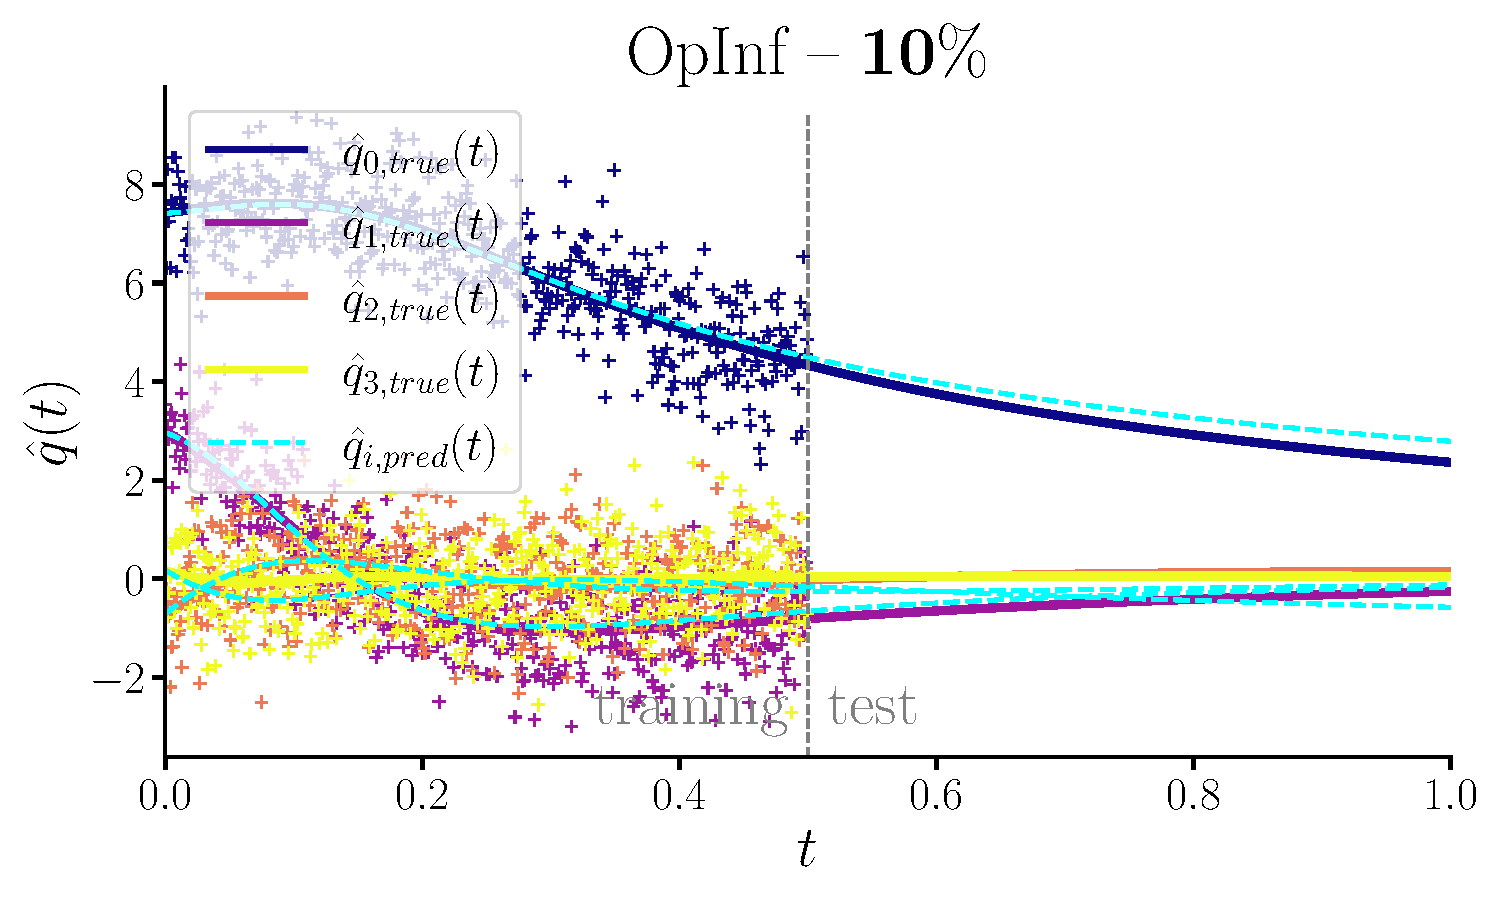
\includegraphics[width=\linewidth]{rom_noise_10_OpInf.pdf}
  \end{subfigure} 
  \begin{subfigure}[c]{0.49\textwidth}
      \centering
      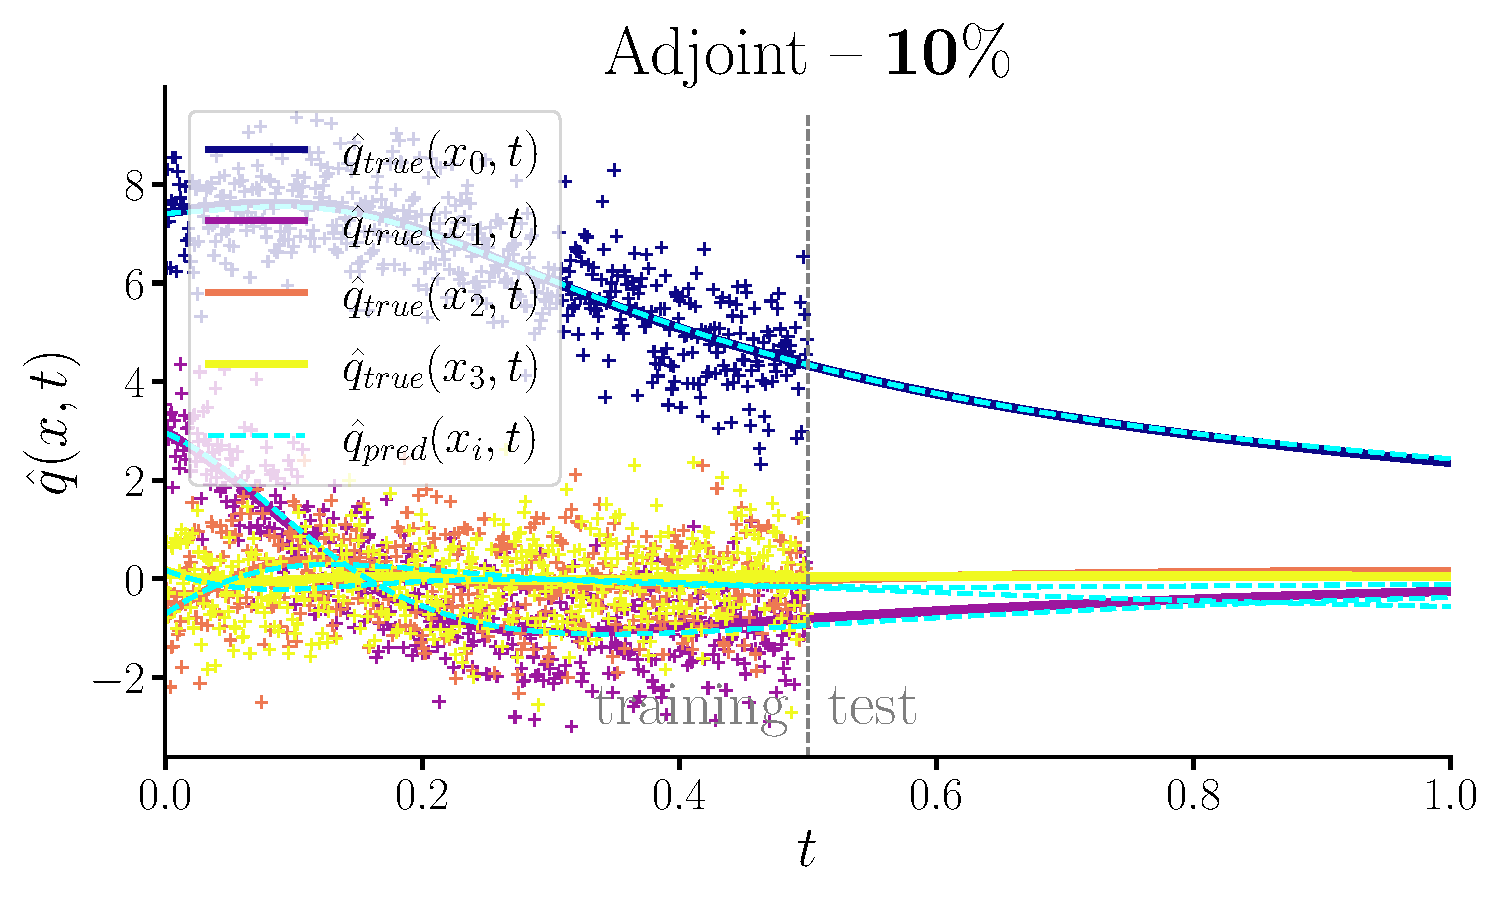
\includegraphics[width=\linewidth]{rom_noise_10_Adj.pdf}
  \end{subfigure} \\[1ex]
    
  \begin{subfigure}[c]{0.49\textwidth}
      \centering
      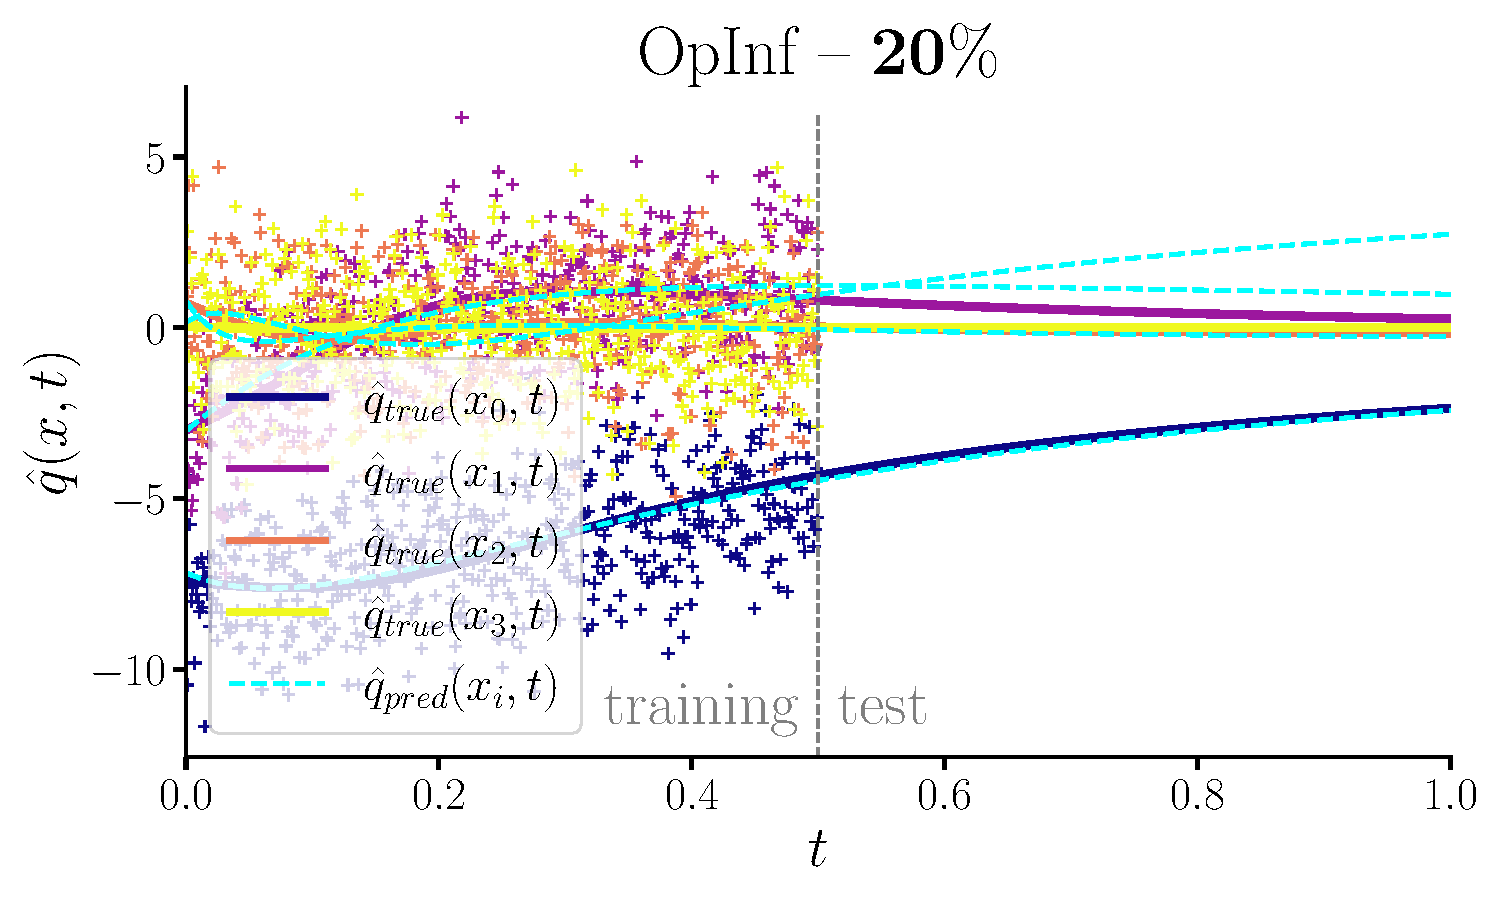
\includegraphics[width=\linewidth]{rom_noise_20_OpInf.pdf}
  \end{subfigure} 
  \begin{subfigure}[c]{0.49\textwidth}
      \centering
      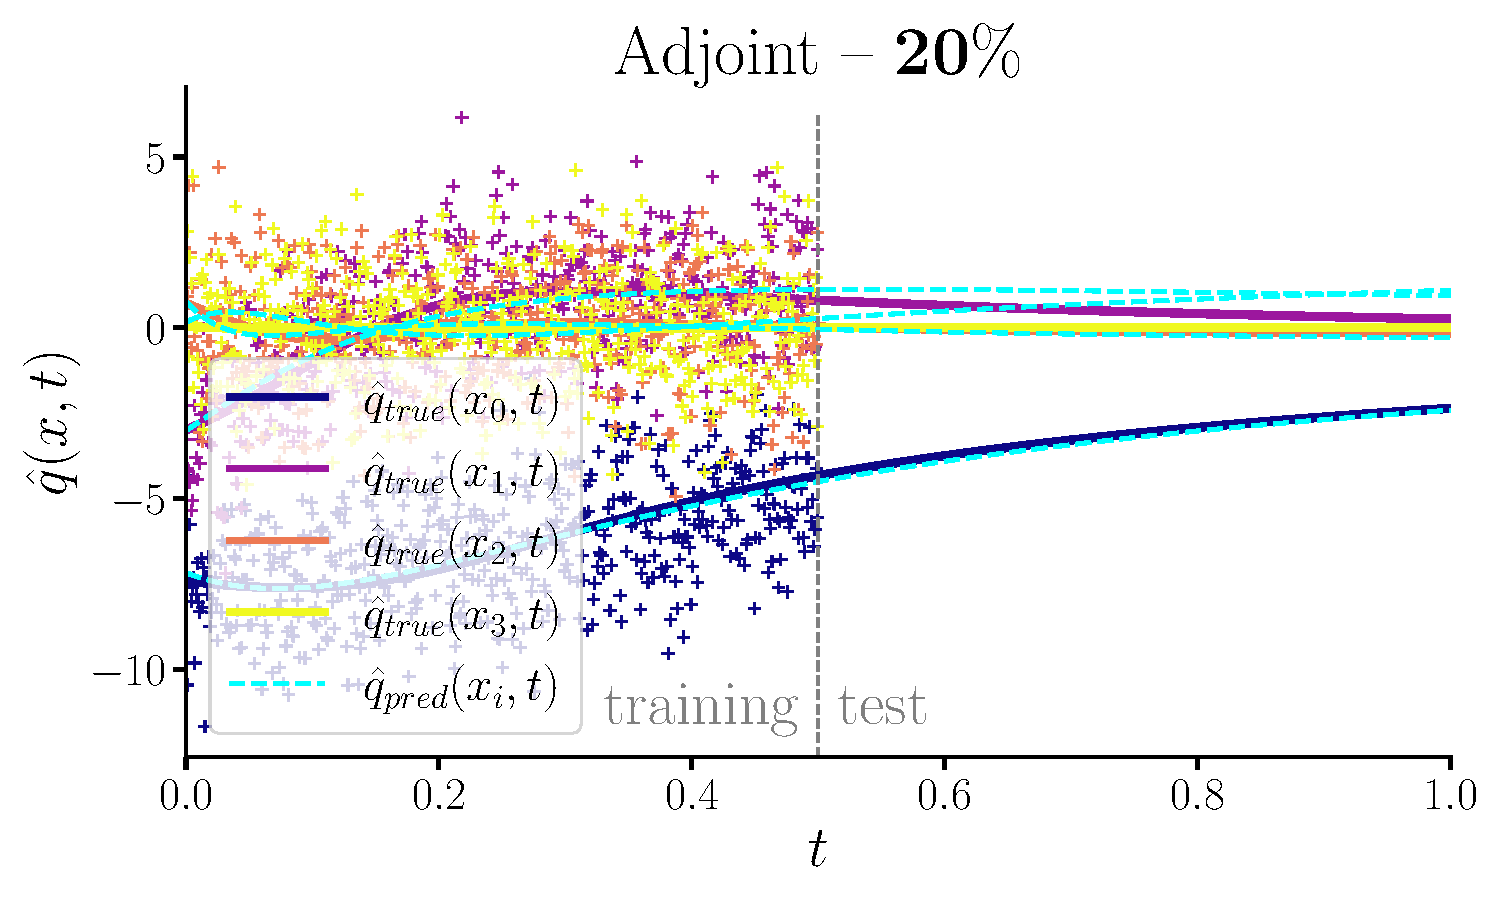
\includegraphics[width=\linewidth]{rom_noise_20_Adj.pdf}
  \end{subfigure} \\[1ex]
  \caption{Noise perturbation simulations for the Burgers' Equation synthetic experiment.}
  \label{fig:five_by_two3}
\end{figure}

\newpage

To assess robustness under imperfect data, we corrupt the full-order snapshots with additive Gaussian noise.  Specifically, we draw\\
$$\mathrm{error} \sim \mathcal{N}\bigl(0,\sigma^2\bigr),
\quad \sigma = \|\mathbf{q}\|_{\mathrm{max}}\,\frac{\text{pct}}{100},$$ 
for noise levels of 1\%, 5\%, 10\%, and 20\%.  Each noisy dataset is then used to train both the OpInf and adjoint models over $t\in[0,0.5]$, with predictions made on $[0.5,1]$. Figure~\ref{fig:five_by_two3} visualizes the true reduced states (scatter and solid) against the trained predictions (dashed) for both methods at each noise level. As noise increases, the adjoint-trained ROM consistently tracks true trajectories more accurately than OpInf, highlighting its superior gradient fidelity in the presence of data corruption.

%%%%%% Prediction Error vs. Time (noise - Burgers) %%%%%%

Figure~\ref{fig:twobytwo3} shows the time-dependent prediction error, as previously defined, for each noise level. While all methods degrade as noise grows, the adjoint method maintains lower errors than both OpInf approaches over time.

\vspace{0.7cm}

\begin{figure}[h!]
  \centering
  
  % First row of subfigures
  \begin{subfigure}[b]{0.48\textwidth}
    \centering
    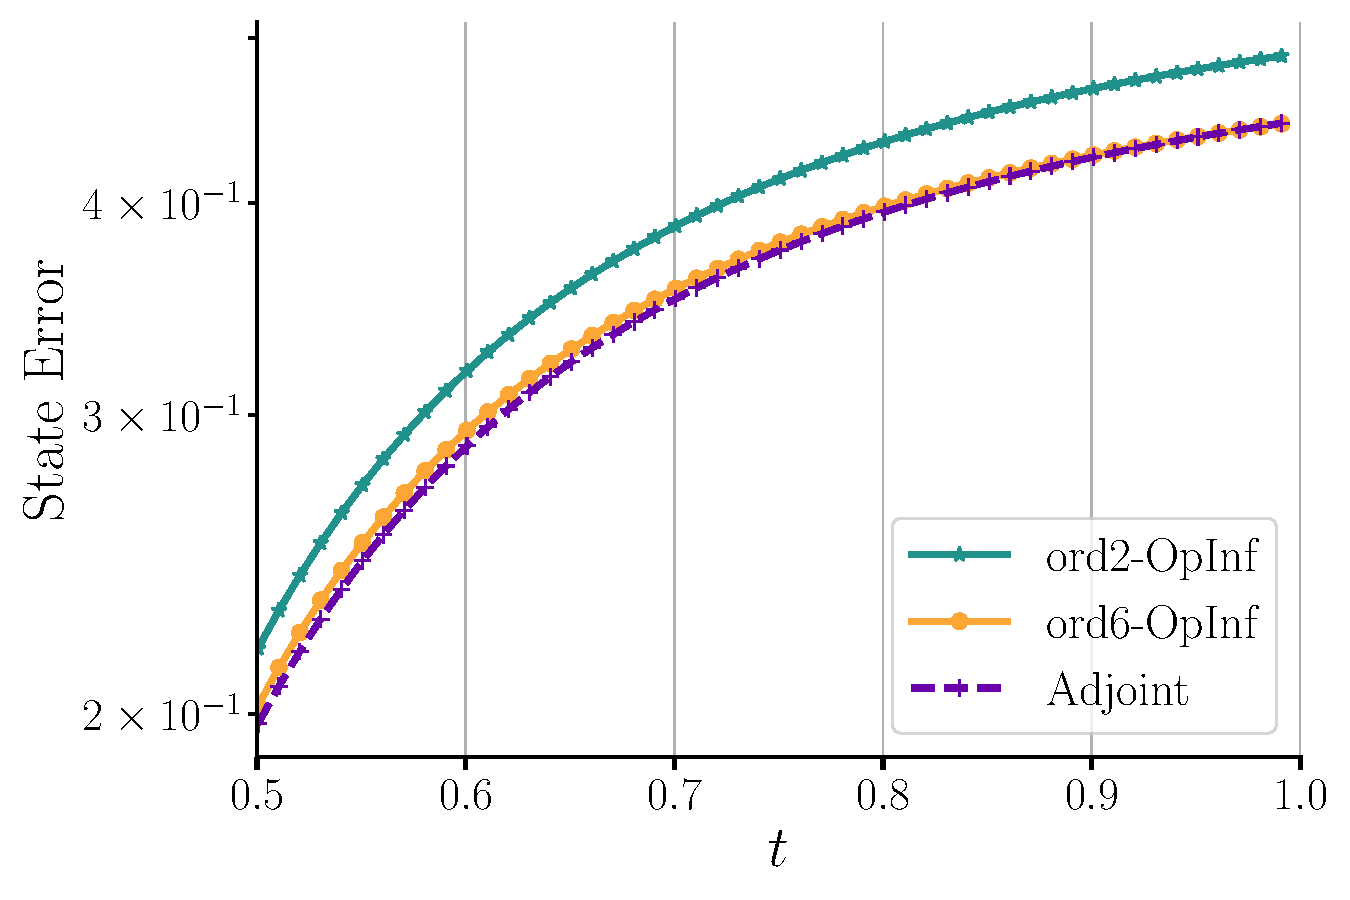
\includegraphics[width=\linewidth]{pred_error_vs_time_noise_1.pdf}
    \caption{1\% of noise level.}
    \label{fig:image1}
  \end{subfigure}
  \quad
  \begin{subfigure}[b]{0.48\textwidth}
    \centering
    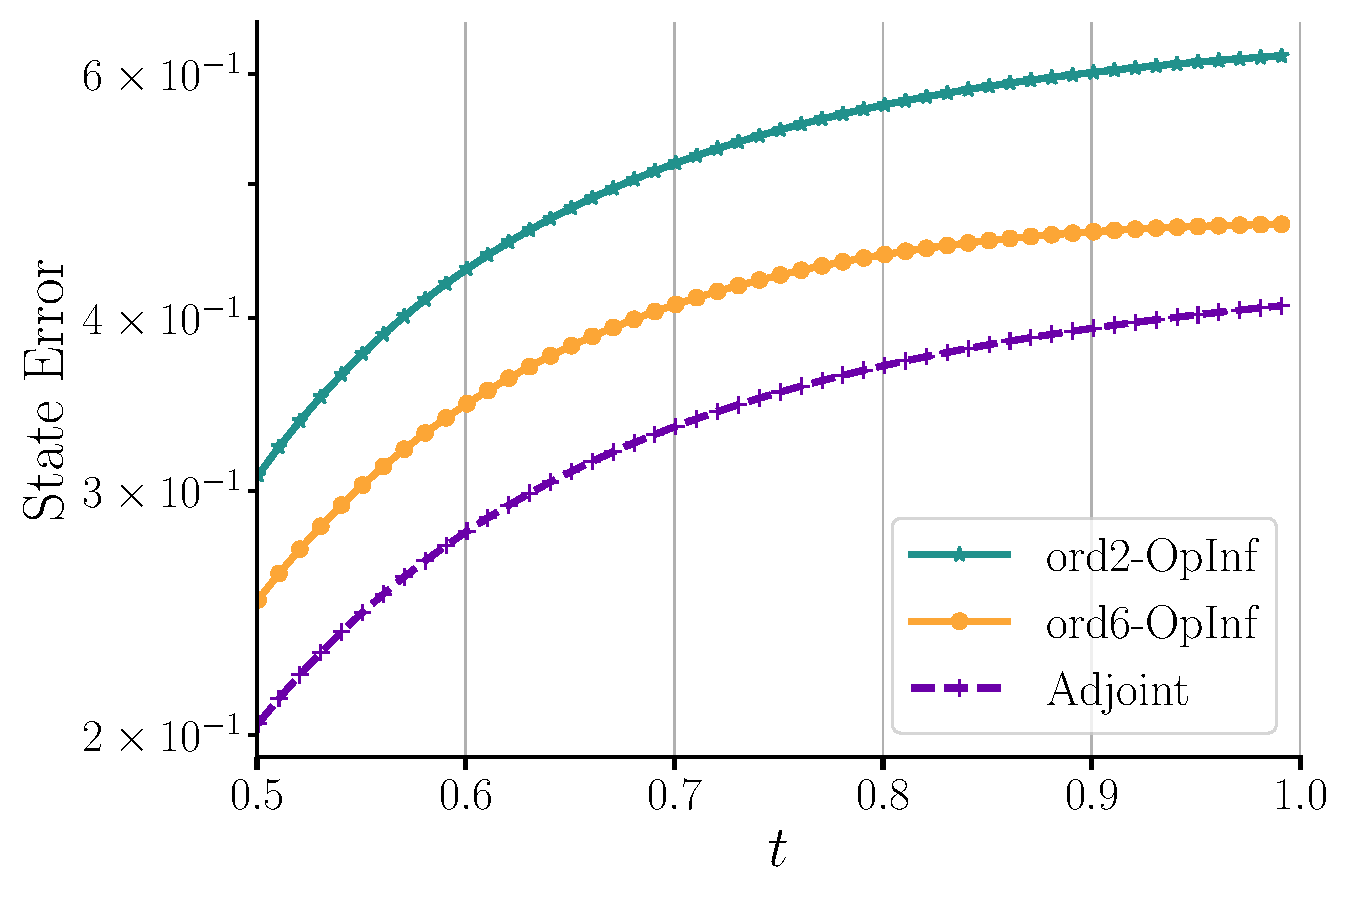
\includegraphics[width=\linewidth]{pred_error_vs_time_noise_5.pdf}
    \caption{5\% of noise level.}
    \label{fig:image2}
  \end{subfigure}
  
  \vskip\baselineskip
  
  % Second row of subfigures
  \begin{subfigure}[b]{0.48\textwidth}
    \centering
    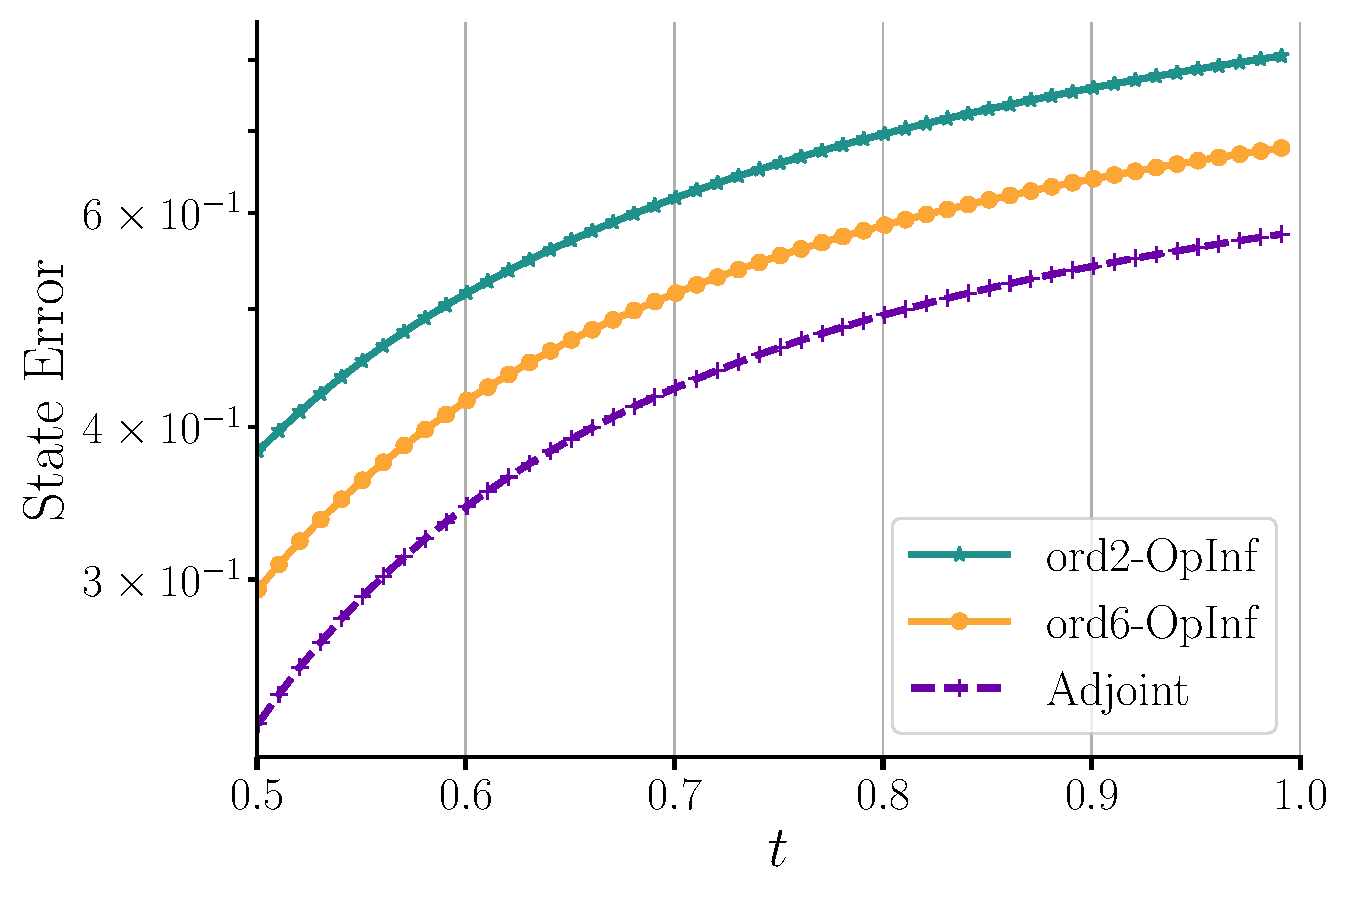
\includegraphics[width=\linewidth]{pred_error_vs_time_noise_10.pdf}
    \caption{10\% of noise level.}
    \label{fig:image3}
  \end{subfigure}
  \quad
  \begin{subfigure}[b]{0.48\textwidth}
    \centering
    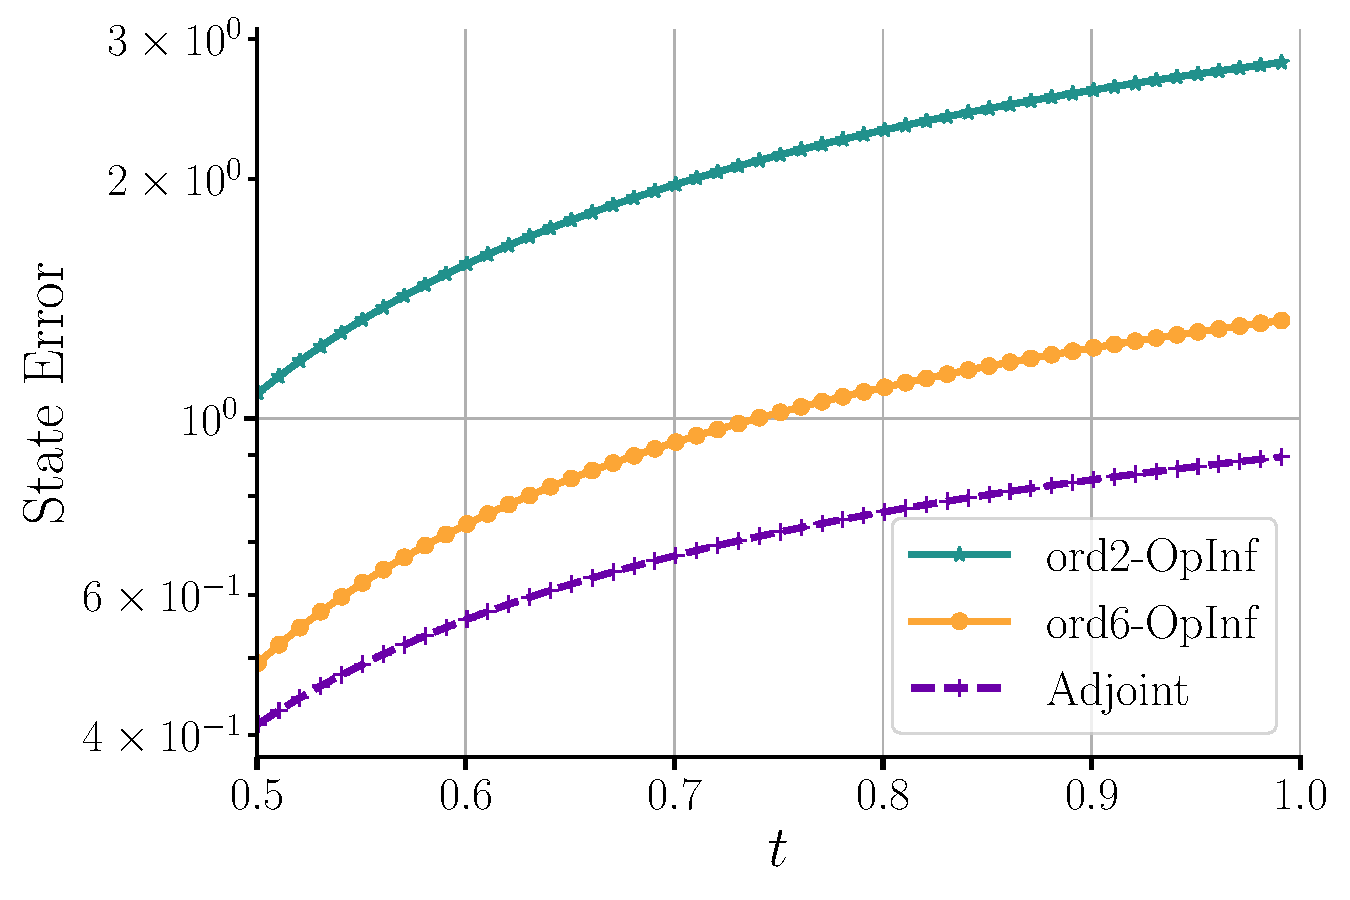
\includegraphics[width=\linewidth]{pred_error_vs_time_noise_20.pdf}
    \caption{20\% of noise level.}
    \label{fig:image4}
  \end{subfigure}
  
  \caption{Prediction error vs. time for each noise level run in the Burgers' Equation experiment.}
  \label{fig:twobytwo3}
\end{figure}

\newpage

%%%%%% Relative Error vs. r (noise - Burgers)%%%%%%

To further quantify model efficiency, Figure~\ref{fig:twobytwo4} plots the relative error as a function of the model dimension $r$. For each noise level, we observe that the adjoint-trained ROM achieves a better accuracy for the same number of modes than both OpInf methods, especially at 5\%, 10\% and 20\% noise.  This confirms that the adjoint gradient yields more informative parameter updates even when training data are corrupted.

\vspace{0.7cm}

\begin{figure}[h!]
  \centering
  
  % First row of subfigures
  \begin{subfigure}[b]{0.48\textwidth}
    \centering
    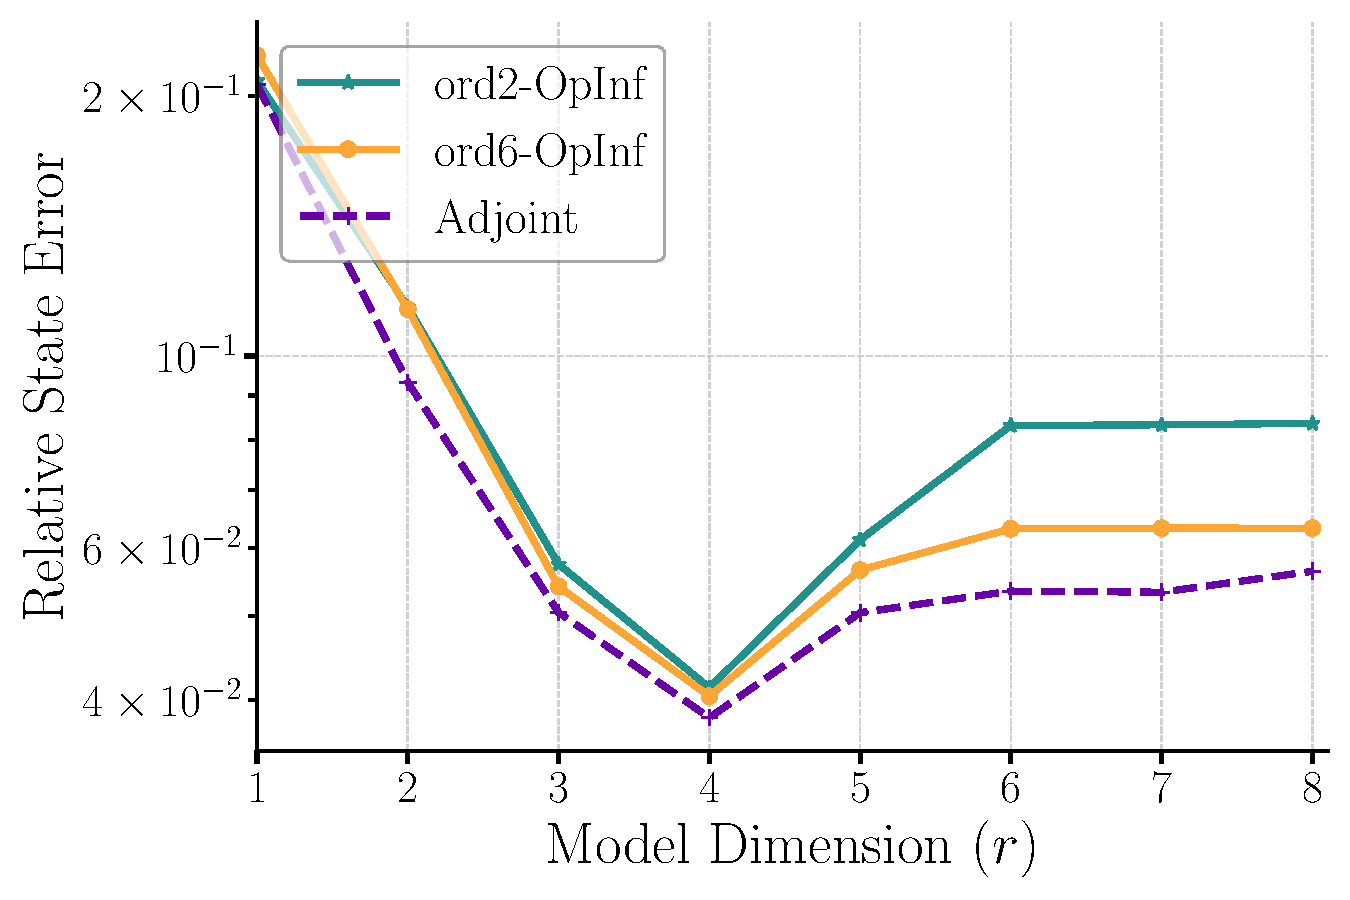
\includegraphics[width=\linewidth]{rel_error_vs_r_noise_1.pdf}
    \caption{1\% of noise level.}
    \label{fig:image1}
  \end{subfigure}
  \quad
  \begin{subfigure}[b]{0.48\textwidth}
    \centering
    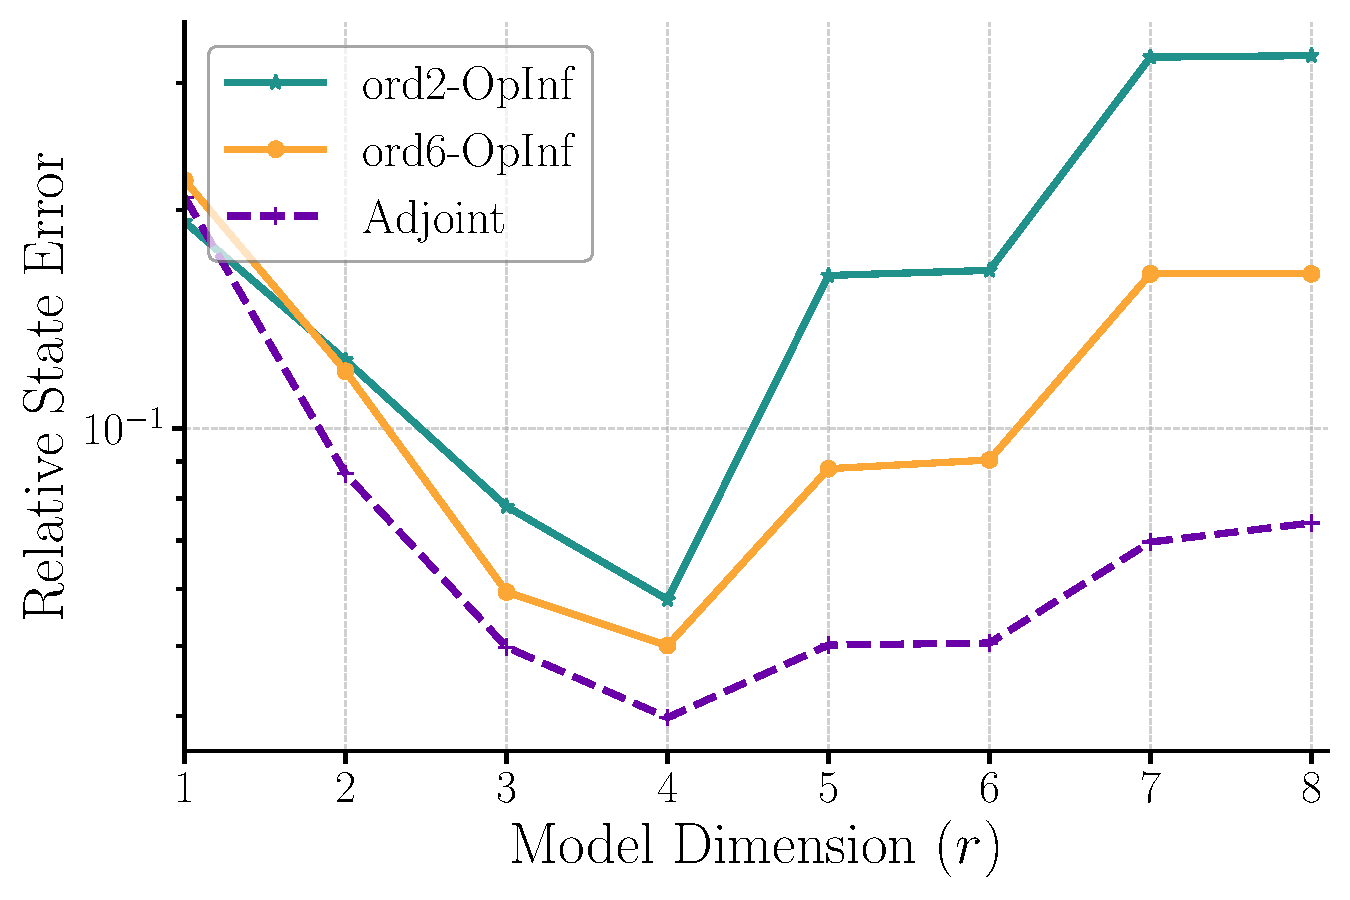
\includegraphics[width=\linewidth]{rel_error_vs_r_noise_5.pdf}
    \caption{5\% of noise level.}
    \label{fig:image2}
  \end{subfigure}
  
  \vskip\baselineskip
  
  % Second row of subfigures
  \begin{subfigure}[b]{0.48\textwidth}
    \centering
    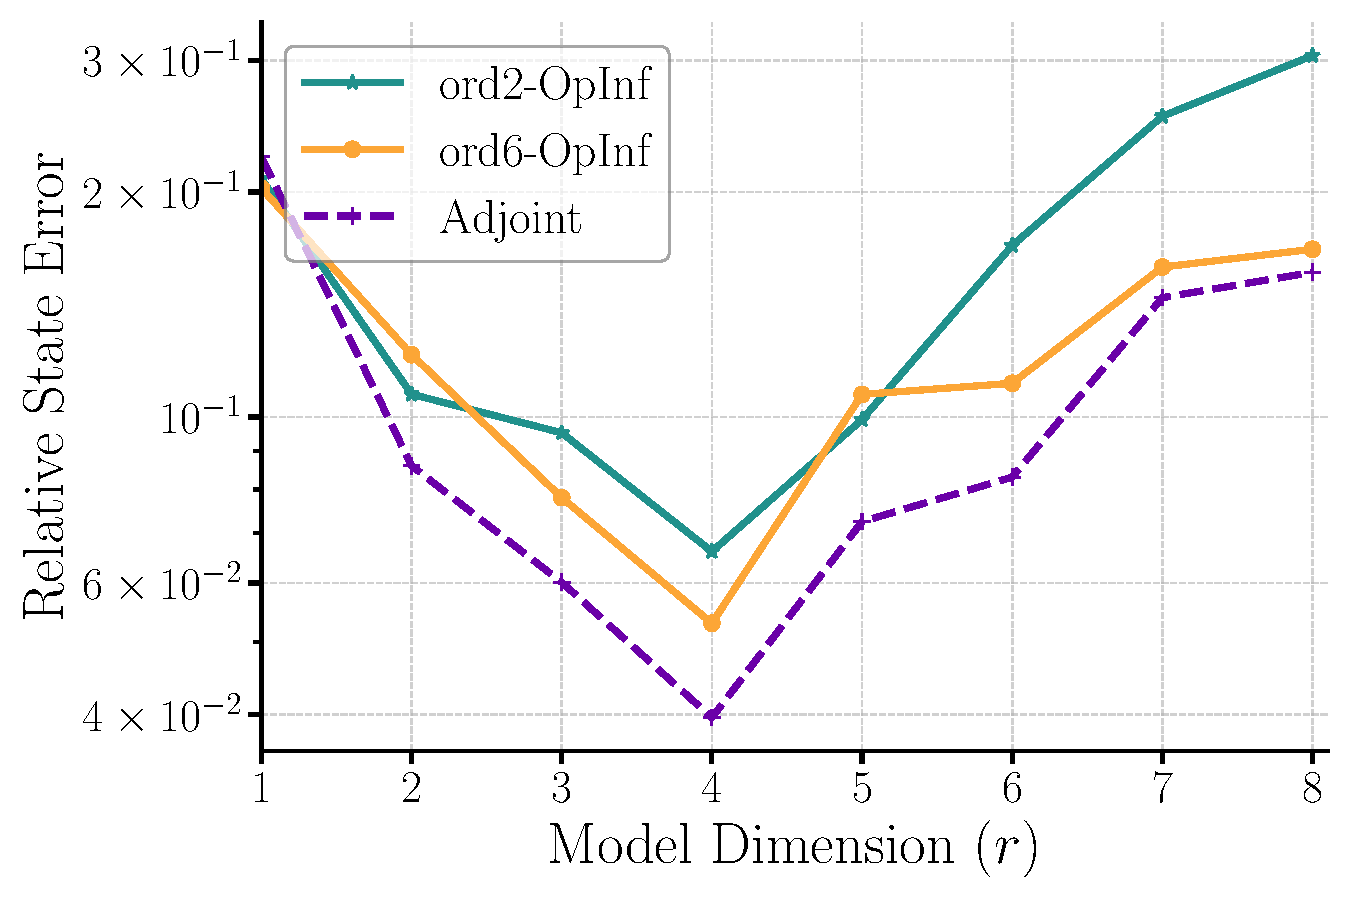
\includegraphics[width=\linewidth]{rel_error_vs_r_noise_10.pdf}
    \caption{10\% of noise level.}
    \label{fig:image3}
  \end{subfigure}
  \quad
  \begin{subfigure}[b]{0.48\textwidth}
    \centering
    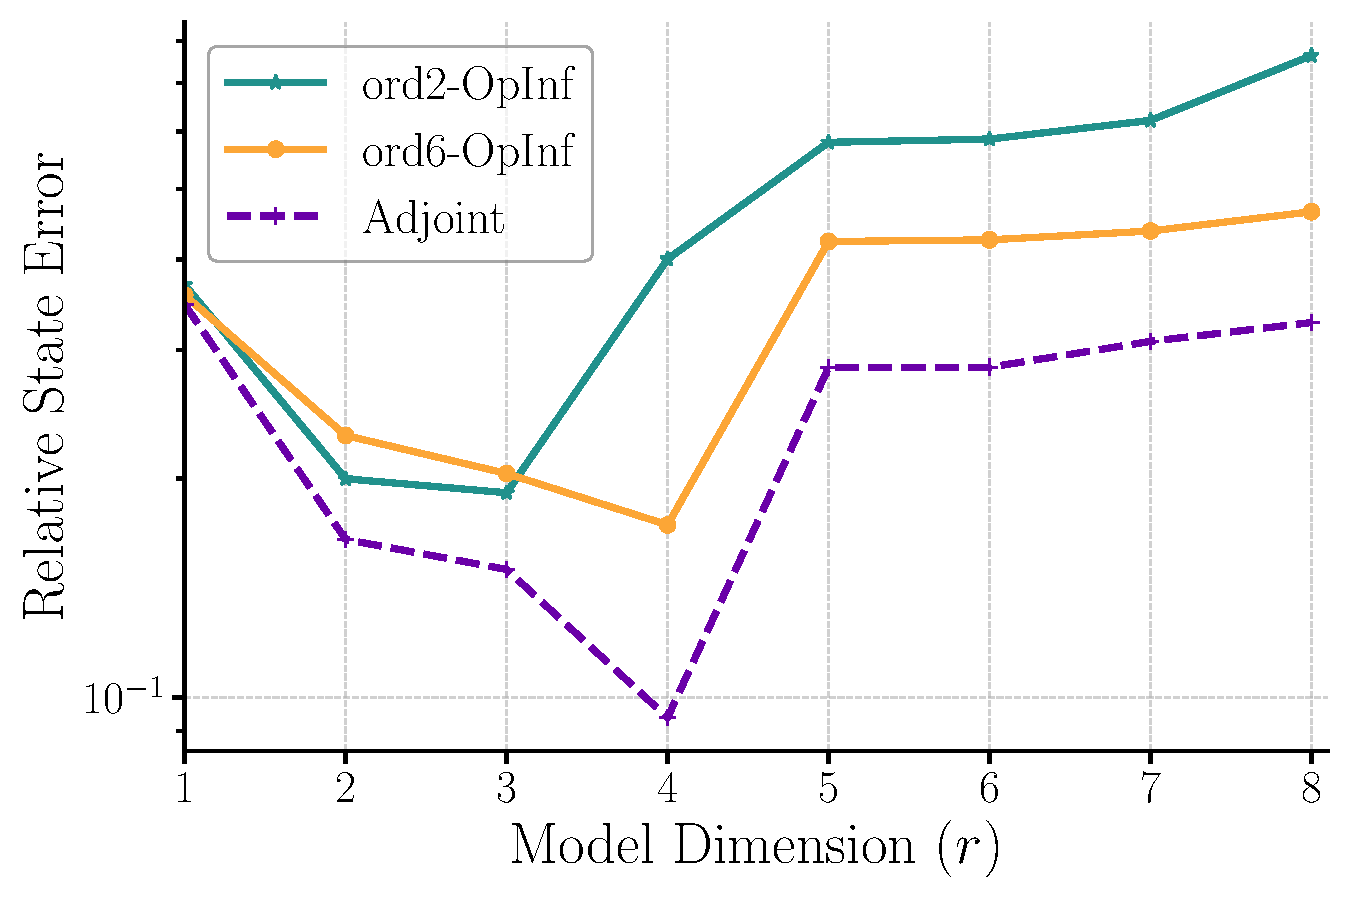
\includegraphics[width=\linewidth]{rel_error_vs_r_noise_20.pdf}
    \caption{20\% of noise level.}
    \label{fig:image4}
  \end{subfigure}
  
  \caption{Relative error vs. $r$ for each noise perturbation run in the Burgers' Equation experiment.}
  \label{fig:twobytwo4}
\end{figure}

\newpage

%%%%%%%%%%%%%%%%%%%%%%%%%%%%%%%%%%%%%%%%%%%%%%%%%%%%%%%%%%%%%%%%%%%%%%%%%%%%%%%%%%%%%%%%%%%%%%
%%%%%%%%%%%%%%%%%%%%%%%%%%%%%%%%%%%%%%%%% FKPP EQUATION %%%%%%%%%%%%%%%%%%%%%%%%%%%%%%%%%%%%%%
%%%%%%%%%%%%%%%%%%%%%%%%%%%%%%%%%%%%%%%%%%%%%%%%%%%%%%%%%%%%%%%%%%%%%%%%%%%%%%%%%%%%%%%%%%%%%%

\section{Fisher-KPP Equation}
\label{sec:fkpp_eq}

\subsection*{Snapshot Data Generation}

For this second synthetic experiment, we generate training data (see code in Appendix \ref{lst:fkpp}) by numerically solving the two-dimensional Fisher-KPP equation,\\
$$q_t = \mathfrak{D}\,(q_{xx} + q_{yy}) \;+\; \rho\,q\,(1 - q), \quad (x,y)\in[0,L_x]\times[0,L_y],\;t\in[0,T],$$
with homogeneous Neumann (zero-flux) boundary conditions\\
$$\frac{\partial q}{\partial n}\Big|_{\partial\Omega} = 0,$$
and a Gaussian initial condition centered in the domain:\\
$$q(x,y,0)= \exp\Bigl(-10\bigl[(x - L_x/2)^2 + (y - L_y/2)^2\bigr]\Bigr).$$

The following parameters and grid are considered:
\begin{itemize}
  \item Domain sizes: $L_x = L_y = 10$.
  \item Grid: $N_x = N_y = 100$ points in each direction, $\Delta x = L_x/(N_x-1)$, $\Delta y = L_y/(N_y-1)$.
  \item Time stepping: final time $T=5$, $\Delta t=0.005$, $N_t = T/\Delta t = 1000$.
  \item Model parameters: diffusion coefficient $\mathfrak{D}=0.1$, logistic growth rate $\rho=1.0$.
\end{itemize}
A finite difference method is then applied for the spatial discretizations:
\begin{itemize}
  \item For the $x$-dimension, we construct a 1D second-difference matrix $\mathbf{L}_x^{1D}\in\mathbb R^{N_x\times N_x}$ with Neumann BCs by\\
$$\bigl(\mathbf{L}_x^{1D}\bigr)_{jj}= -\frac{2}{\Delta x^2}, \quad \bigl(\mathbf{L}_x^{1D}\bigr)_{j,j\pm1}= \frac{1}{\Delta x^2},
      \quad (\mathbf{L}_x^{1D})_{0,1} = (\mathbf{L}_x^{1D})_{N_x-1,N_x-2} = \frac{2}{\Delta x^2}.$$
  \item Similarly, we define \(\mathbf{L}_y^{1D}\in\mathbb R^{N_y\times N_y}\) on the \(y\)-grid.
  \item Both expressions are combined to form a full 2D-Laplacian by Kronecker sums\\
    $$\mathbf{L} = \mathbf{I}_{N_y}\otimes \mathbf{L}_x^{1D} \;+\; \mathbf{L}_y^{1D}\otimes \mathbf{I}_{N_x}\quad\in\mathbb R^{(N_xN_y)\times(N_xN_y)}.$$
\end{itemize}
For the time-stepping scheme, we use a semi-implicit Crank-Nicolson step for the diffusion and explicit Euler for the reaction term:\\
$$\dfrac{\mathbf{q}^{m+1} - \mathbf{q}^{m}}{\Delta t} = \dfrac{\mathfrak{D}}{2}\mathbf{L}(\mathbf{q}^{m+1}+\mathbf{q}^m)\;+\,\rho\,\mathbf{q}^m\circ(\mathbf{1} - \mathbf{q}^m),$$ 
where $\circ$ denotes the Hadamard product.

By defining,
$$\alpha \;\coloneqq\;\frac{\mathfrak{D}\,\Delta t}{2}, \quad \bm{\mathcal{A}} \;\coloneqq\; \mathbf{I} - \alpha\,\mathbf{L}, \quad \bm{\mathcal{B}} \;\coloneqq\; \mathbf{I} + \alpha\,\mathbf{L},$$
then at each time step\\
$$\bm{\mathcal{A}}\mathbf{q}^{m+1} = \bm{\mathcal{B}}\mathbf{q}^m + \Delta t\,\rho\,\mathbf{q}^m\circ(\mathbf{1} - \mathbf{q}^m).$$
By solving this sparse linear system we get the desired state solution at every time step that we will use to build the snapshot matrix
$\mathbf{Q}\in\mathbb R^{(N_xN_y)\times N_t}.$

Visualization of the dynamics for the Fisher-KPP equation is shown in Figure~\ref{fig:fisher-data}.

\begin{figure}[h!]
    \hspace{-0.8cm}
  \centering
  \begin{subfigure}[t]{\textwidth}
    \centering
    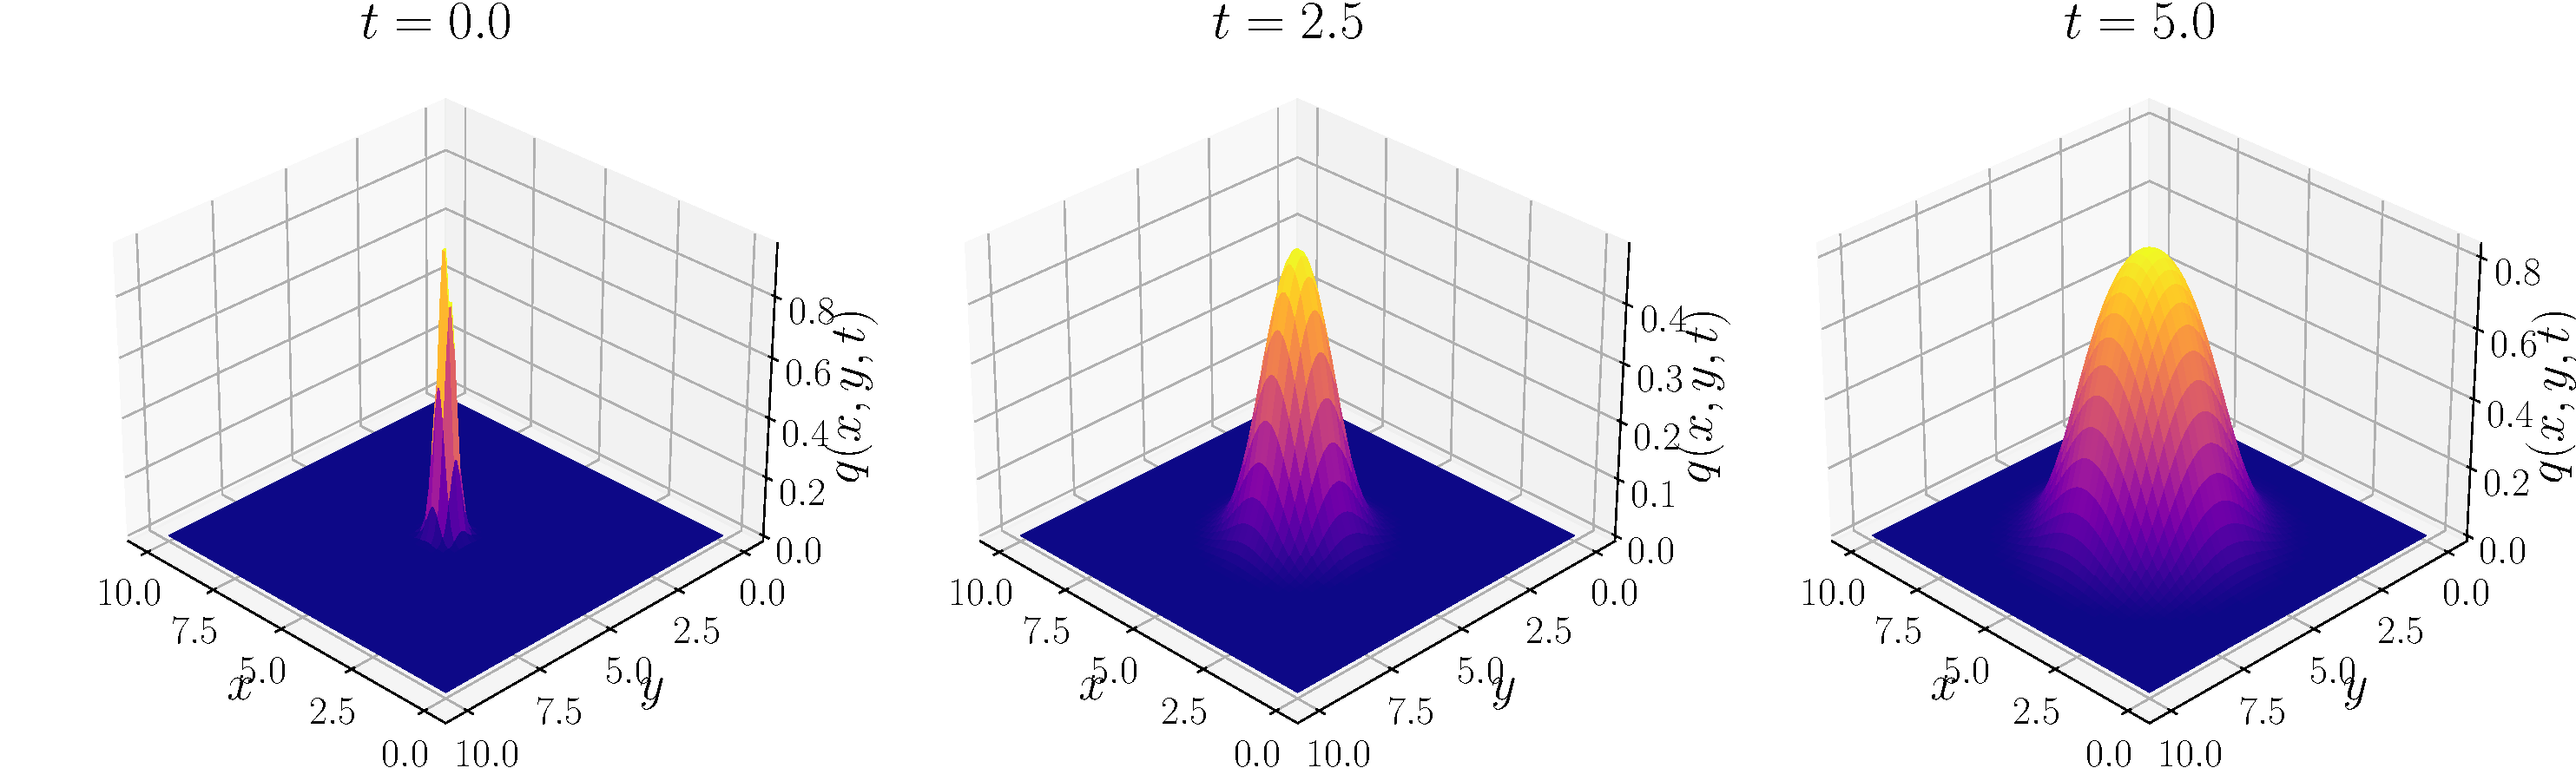
\includegraphics[width=\textwidth]{3Dfkpp.pdf}
    \caption{3D surface of $q(x,y,t)$ for $\mathfrak{D}=0.1$ and $\rho=1$.}
    \label{fig:fisher-init}
  \end{subfigure}
  \\[1em]
  \begin{subfigure}[t]{0.48\textwidth}
    \centering
    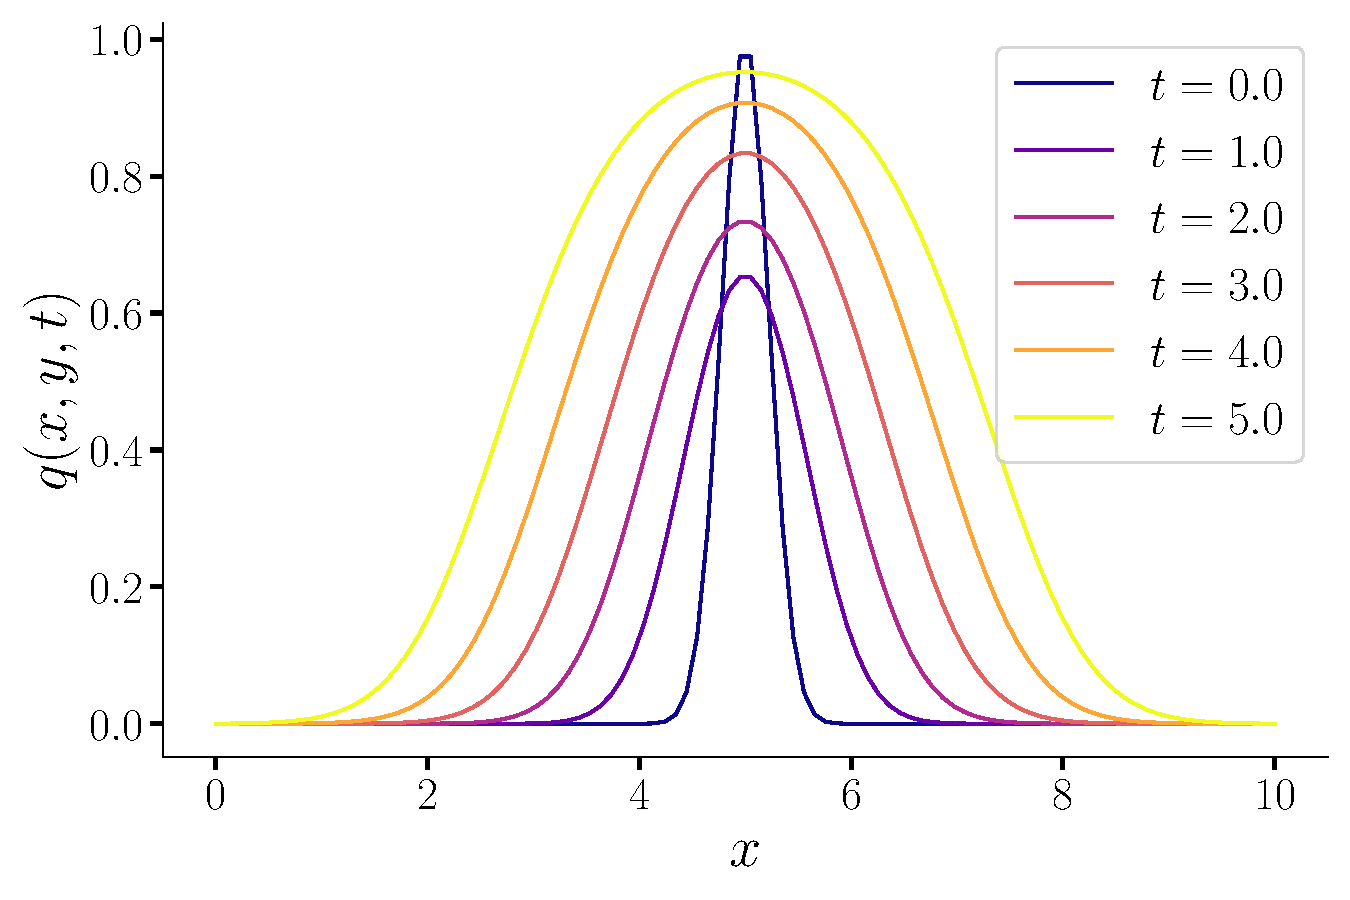
\includegraphics[width=\textwidth]{1Dfkpp.pdf}
    \caption{Profiles of $q(x.y.t)$ for different $t_k$.}
    \label{fig:fisher-mid}
  \end{subfigure}
  \hfill
  \begin{subfigure}[t]{0.48\textwidth}
    \centering
    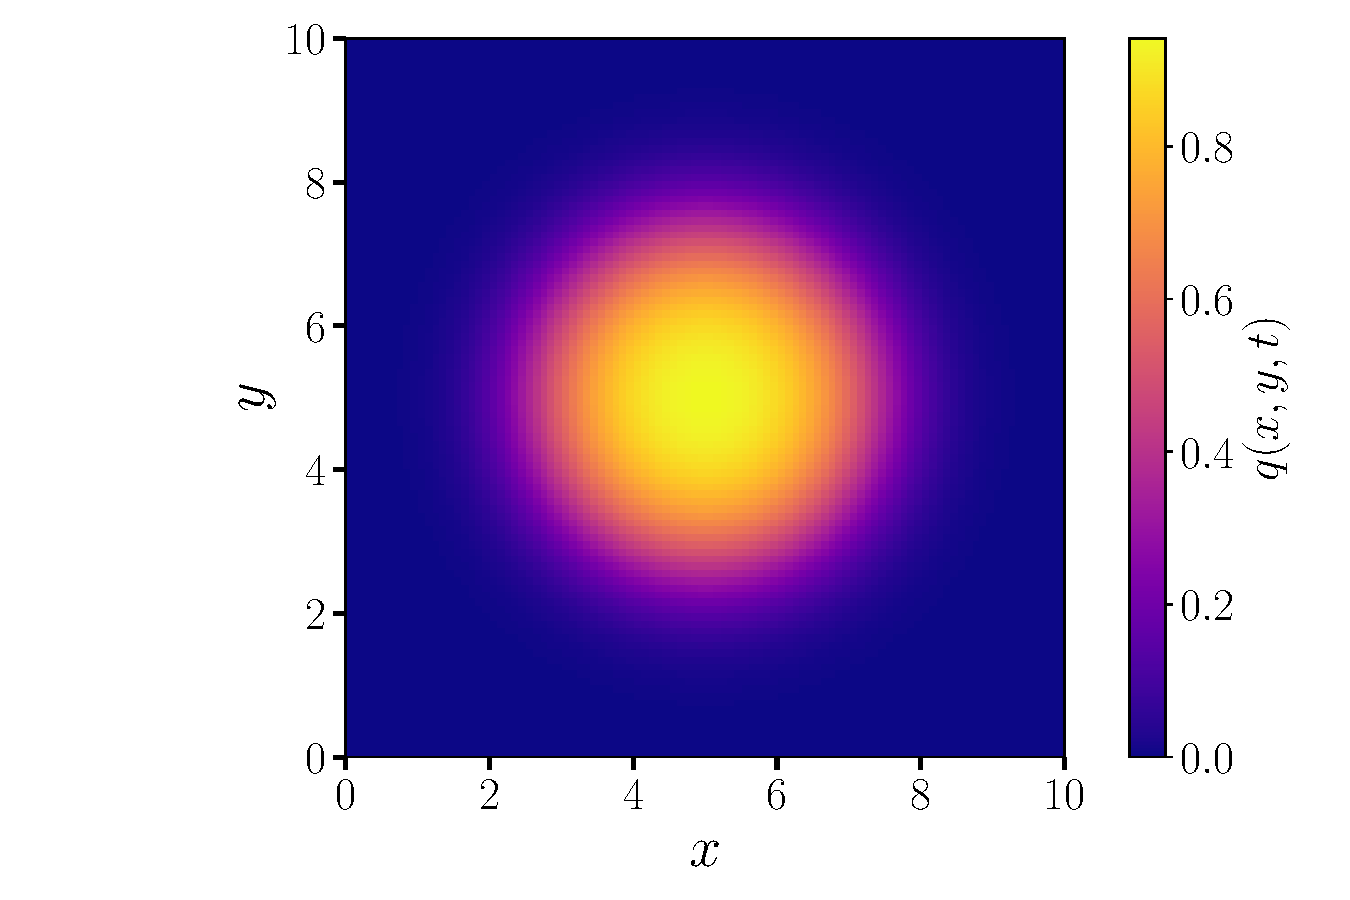
\includegraphics[width=\textwidth]{2Dfkpp.pdf}
    \caption{Space-time contour of $q(x,y,t)$ at $t=5$.}
    \label{fig:fisher-final}
  \end{subfigure}
  \caption{Dynamics of the FKPP equation used for data generation.}
  \label{fig:fisher-data}
\end{figure}     

\newpage

%%%%%%%%%%%%%%%%%%%%%%%%%%%%%%%%% NOISE PERTURBATION %%%%%%%%%%%%%%%%%%%%%%%%%%%%%%%%%%

\subsection*{Noise Perturbation}

\vspace{1.0cm}

\begin{figure}[h!]
  \centering
  \begin{subfigure}[c]{0.49\textwidth}
      \centering
      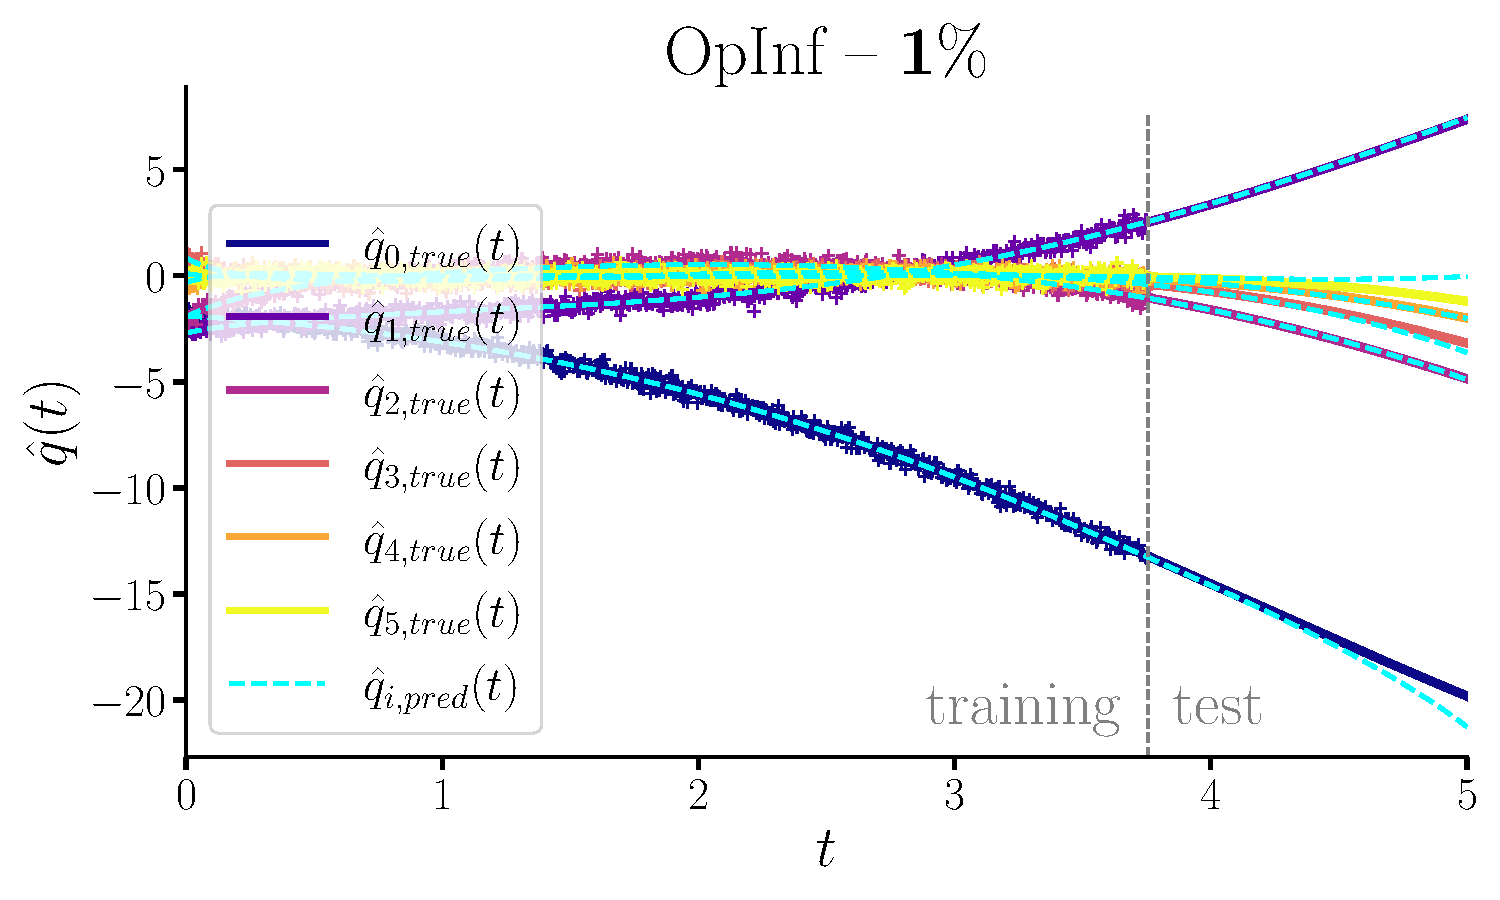
\includegraphics[width=\linewidth]{fkpp_rom_noise_1_OpInf.pdf}
  \end{subfigure}
  \begin{subfigure}[c]{0.49\textwidth}
      \centering
      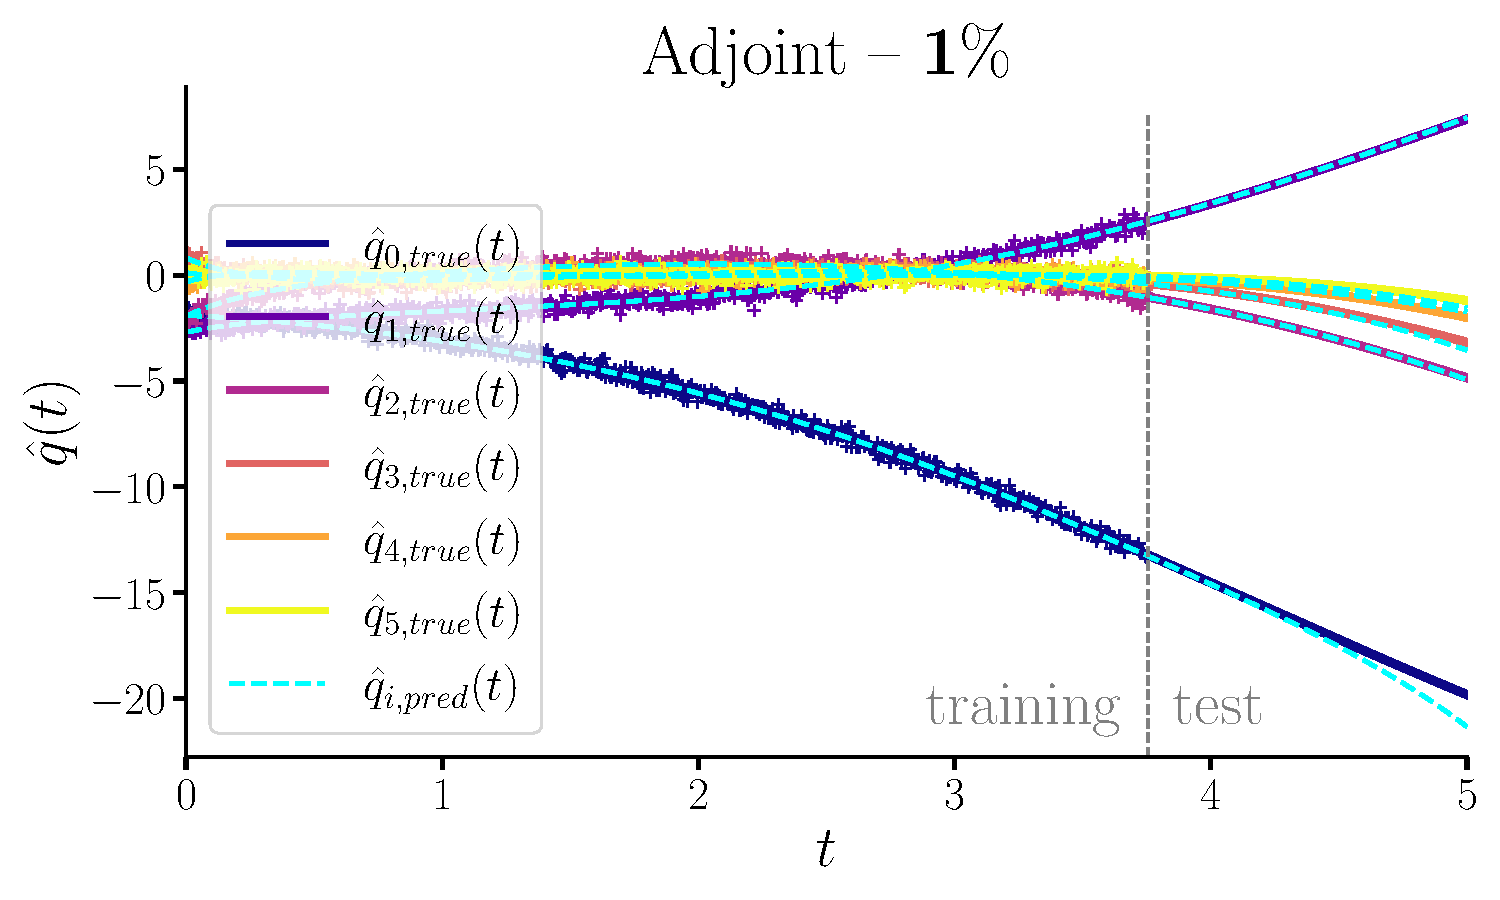
\includegraphics[width=\linewidth]{fkpp_rom_noise_1_Adj.pdf}
  \end{subfigure} \\[1ex]
    
  \begin{subfigure}[c]{0.49\textwidth}
      \centering
      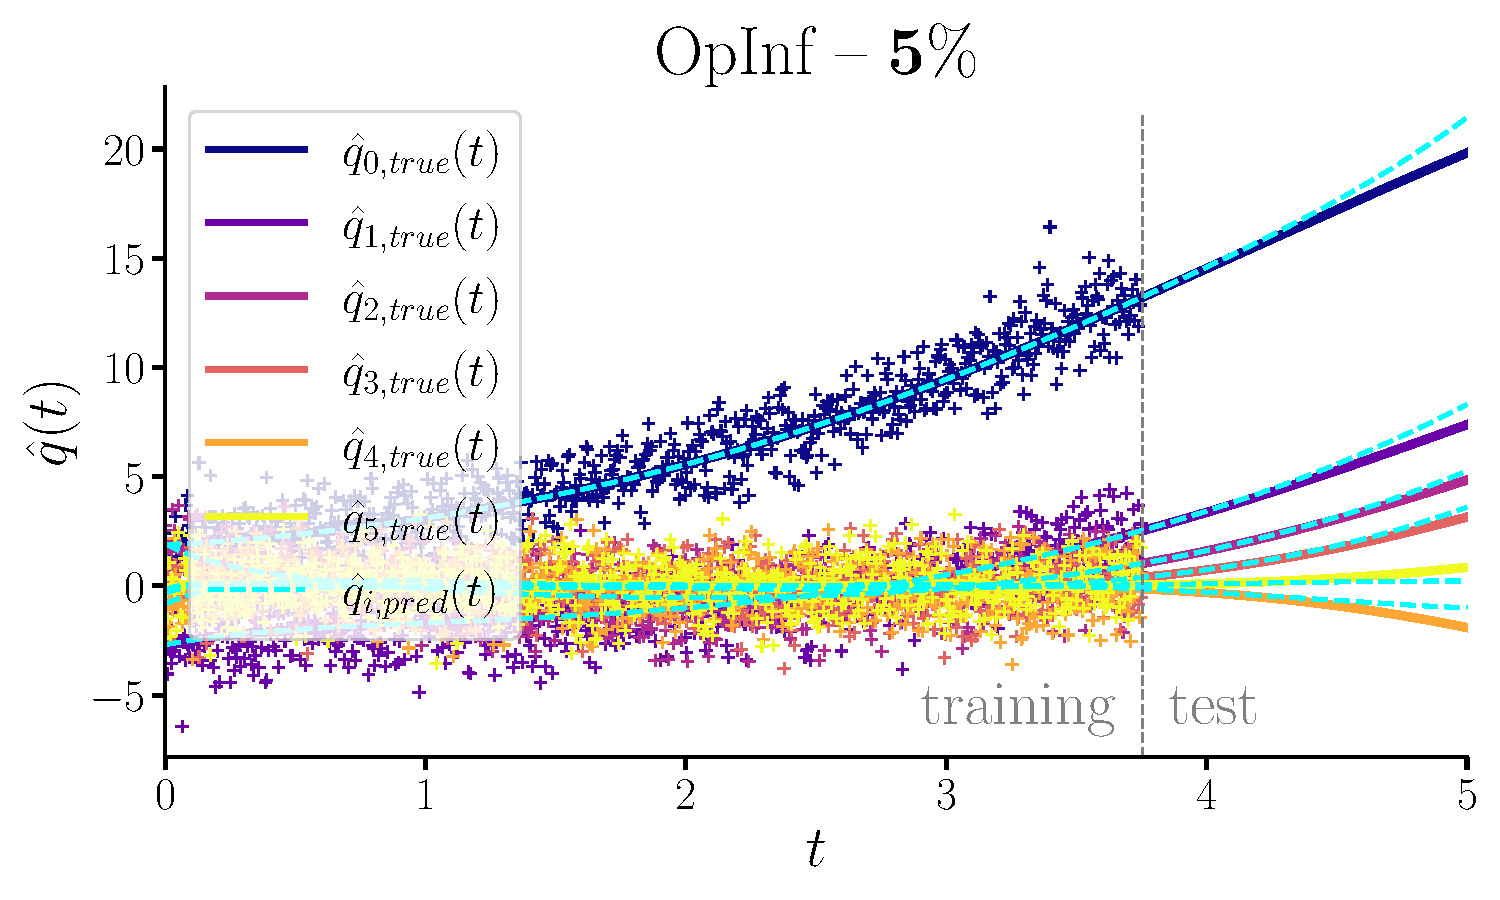
\includegraphics[width=\linewidth]{fkpp_rom_noise_5_OpInf.pdf}
  \end{subfigure} 
  \begin{subfigure}[c]{0.49\textwidth}
      \centering
      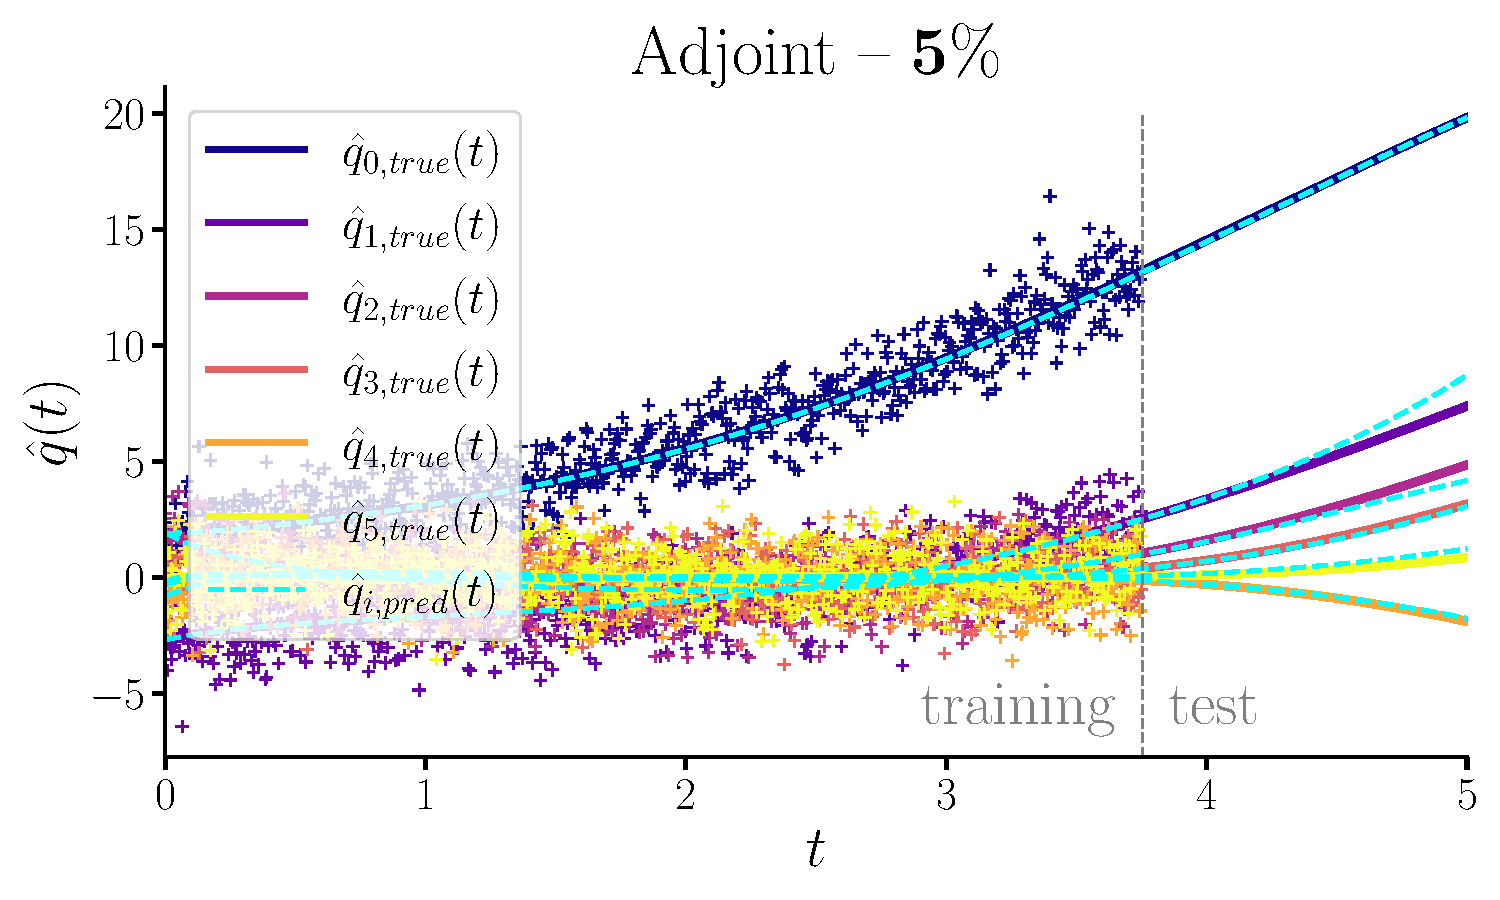
\includegraphics[width=\linewidth]{fkpp_rom_noise_5_Adj.pdf}
  \end{subfigure} \\[1ex]
    
  \begin{subfigure}[c]{0.49\textwidth}
      \centering
      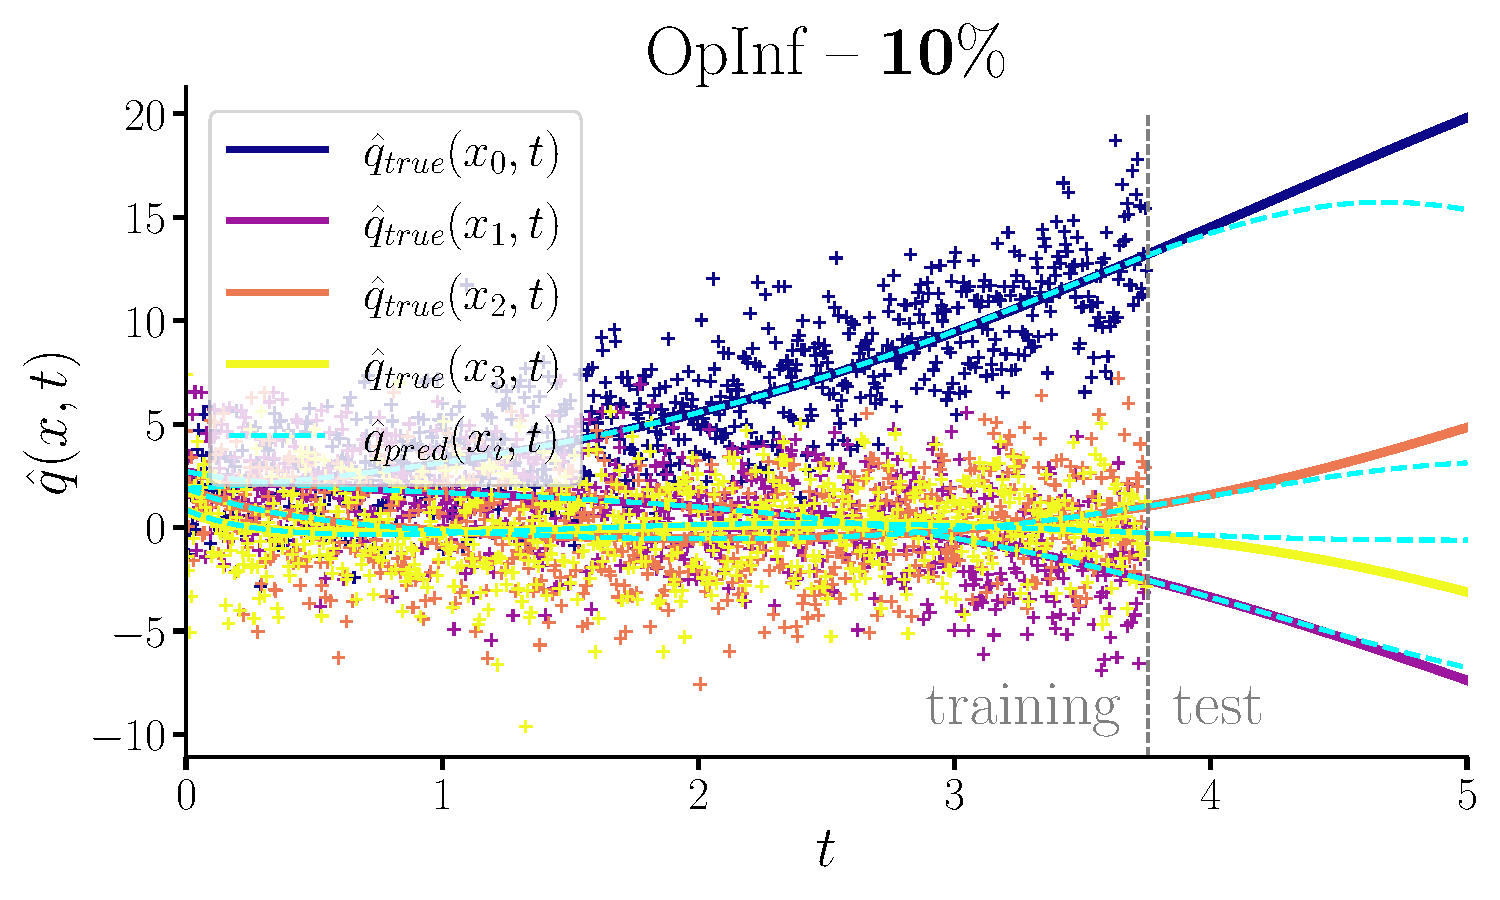
\includegraphics[width=\linewidth]{fkpp_rom_noise_10_OpInf.pdf}
  \end{subfigure} 
  \begin{subfigure}[c]{0.49\textwidth}
      \centering
      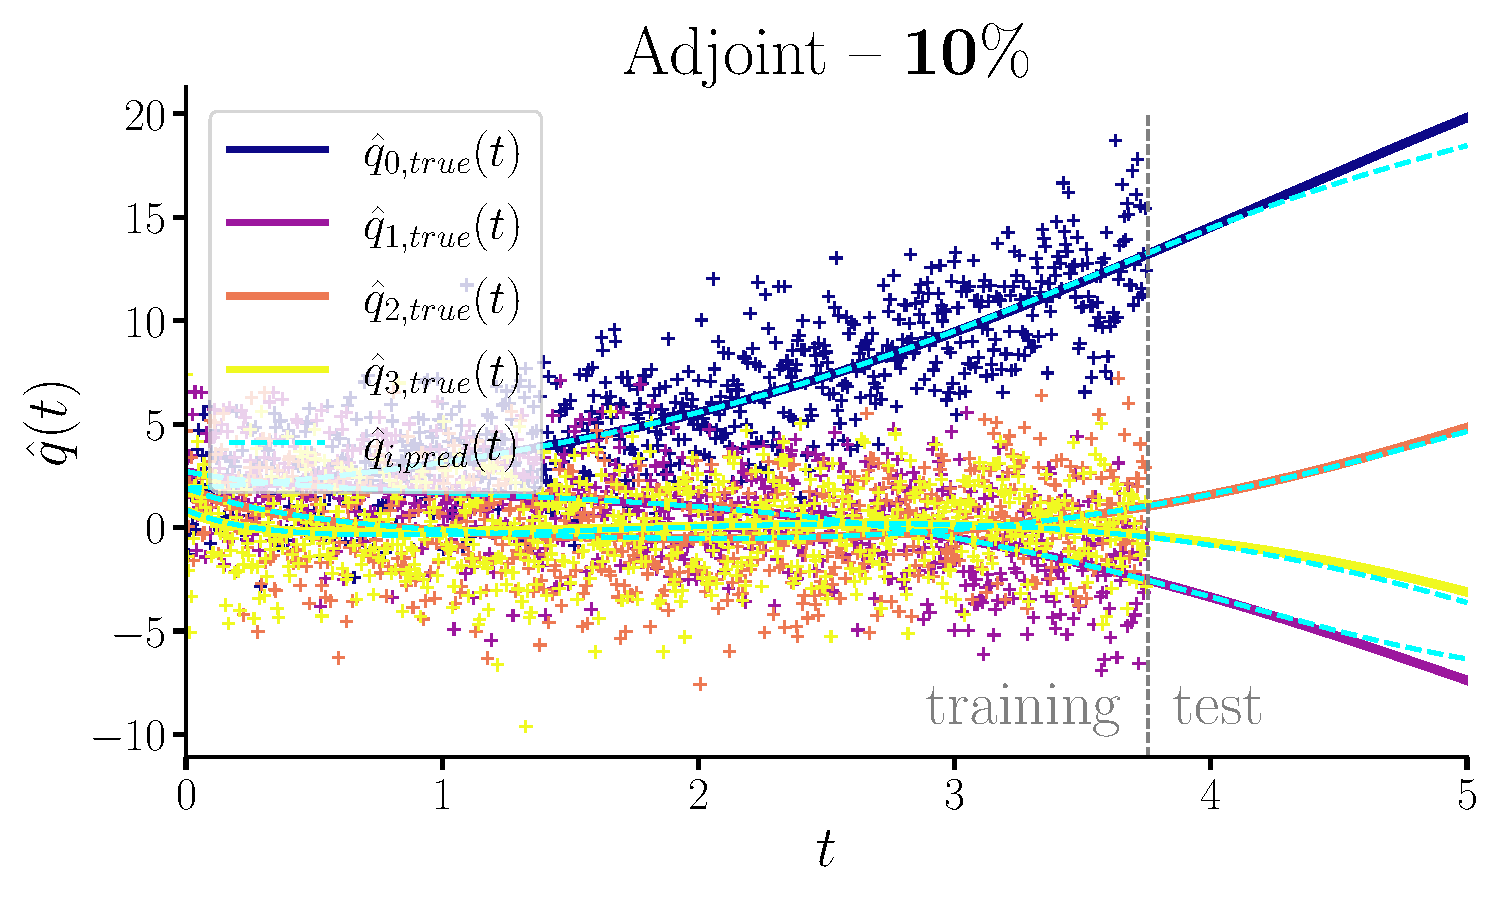
\includegraphics[width=\linewidth]{fkpp_rom_noise_10_Adj.pdf}
  \end{subfigure} \\[1ex]
    
  \begin{subfigure}[c]{0.49\textwidth}
      \centering
      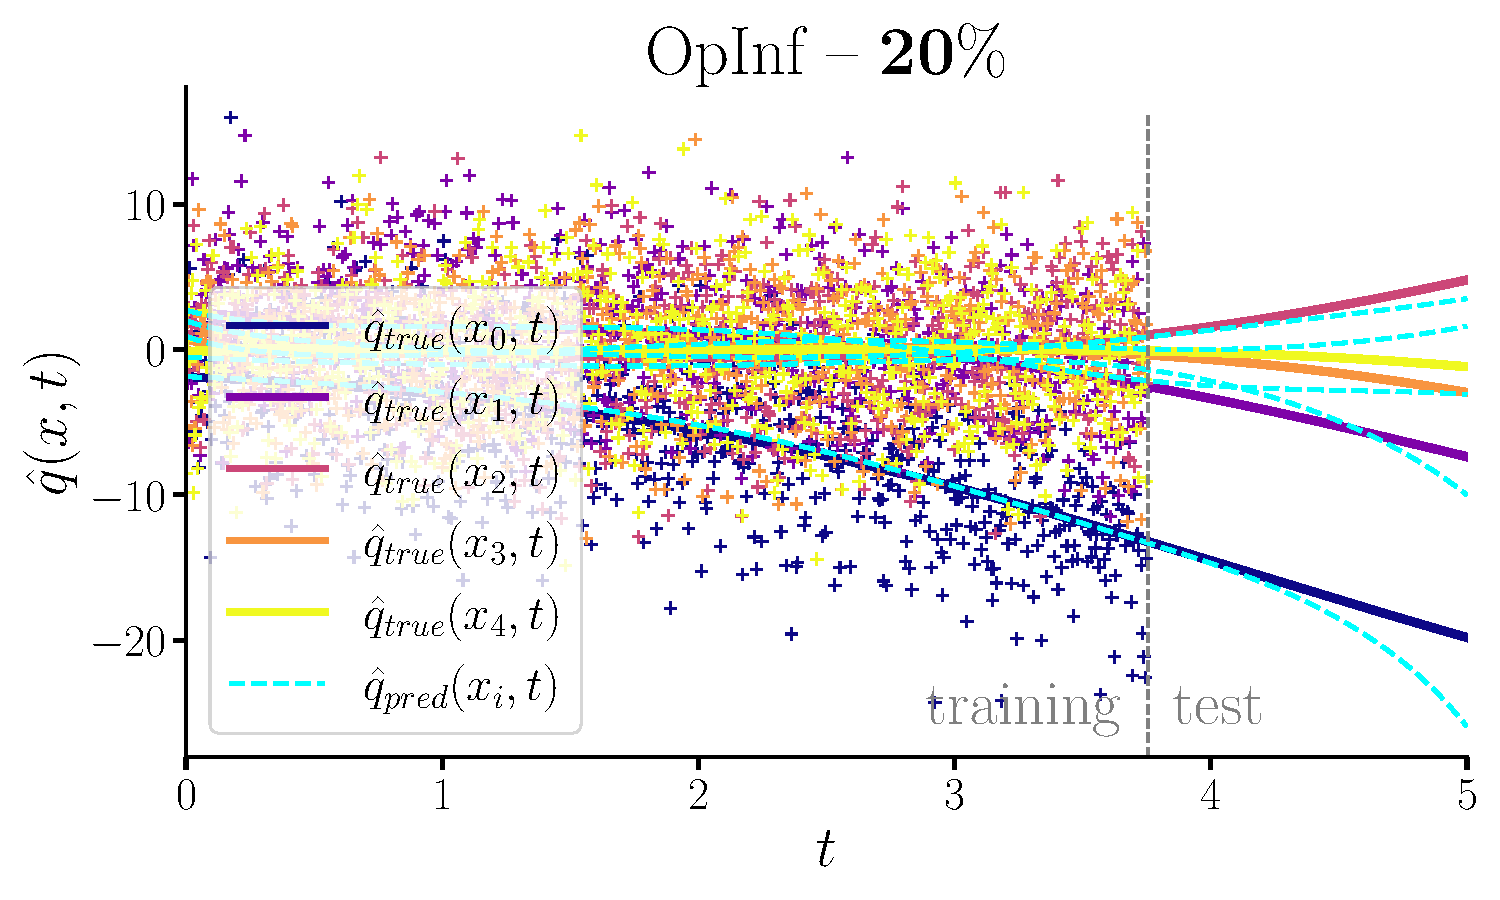
\includegraphics[width=\linewidth]{fkpp_rom_noise_20_OpInf.pdf}
  \end{subfigure} 
  \begin{subfigure}[c]{0.49\textwidth}
      \centering
      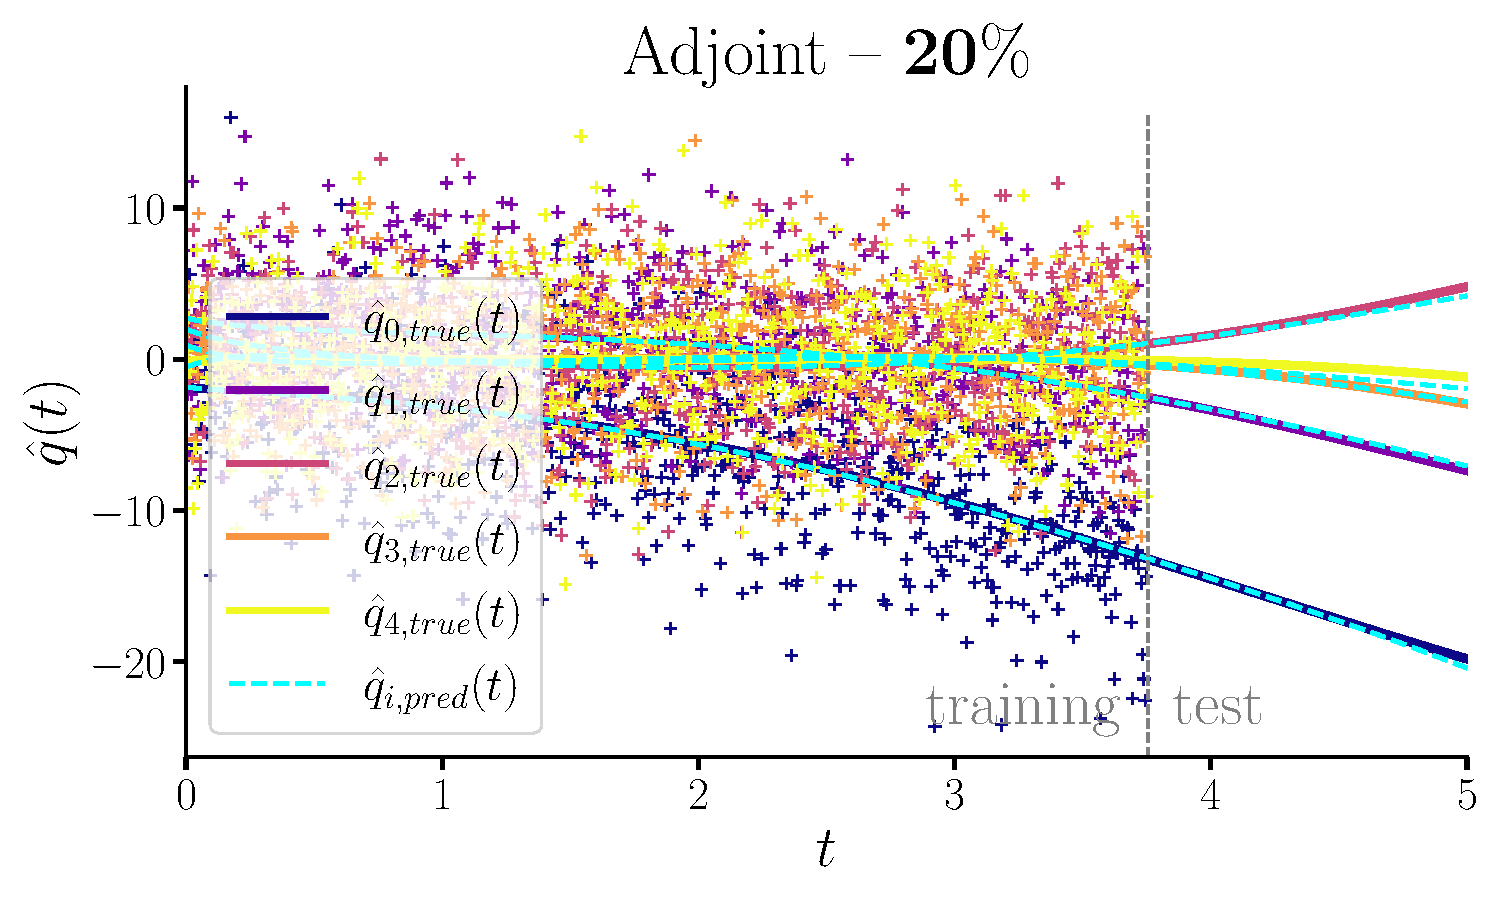
\includegraphics[width=\linewidth]{fkpp_rom_noise_20_Adj.pdf}
  \end{subfigure} \\[1ex]
  \caption{Noise perturbation simulations for the FKPP Equation synthetic experiment.}
  \label{fig:five_by_two4}
\end{figure}

\newpage

%Global summary for FKPP noise experiments%

In the case of the 2D Fisher-KPP equation, we omit the data density reduction study since it yielded virtually the same conclusions as for Burgers' with no significant performance gap between sixth-order OpInf and the adjoint method. Instead, we focus solely on the noise perturbation results, which are displayed in Figures~\ref{fig:five_by_two4}, \ref{fig:twobytwo5}, and \ref{fig:twobytwo6}. Due to stability considerations in the reaction-diffusion dynamics, we extended in this case the training window to cover 75\% of the total simulation time.

Across all four noise levels (1\%, 5\%, 10\%, and 20\%), the adjoint-trained ROM consistently outperformed the best OpInf configuration (\texttt{'ord6'}), both in trajectory fidelity and in error metrics. 

%%%%%% Prediction Error vs. Time (noise - FKPP) %%%%%%

In the time-series comparisons of the reduced states (Figure~\ref{fig:twobytwo5}), the corresponding prediction-error curves confirm that the adjoint approach maintains lower error evolution over the prediction interval, especially at the highest noise levels, where the estimates of the finite difference derivative degrade significantly.

\vspace{0.7cm}

\begin{figure}[h!]
  \centering
  
  % First row of subfigures
  \begin{subfigure}[b]{0.48\textwidth}
    \centering
    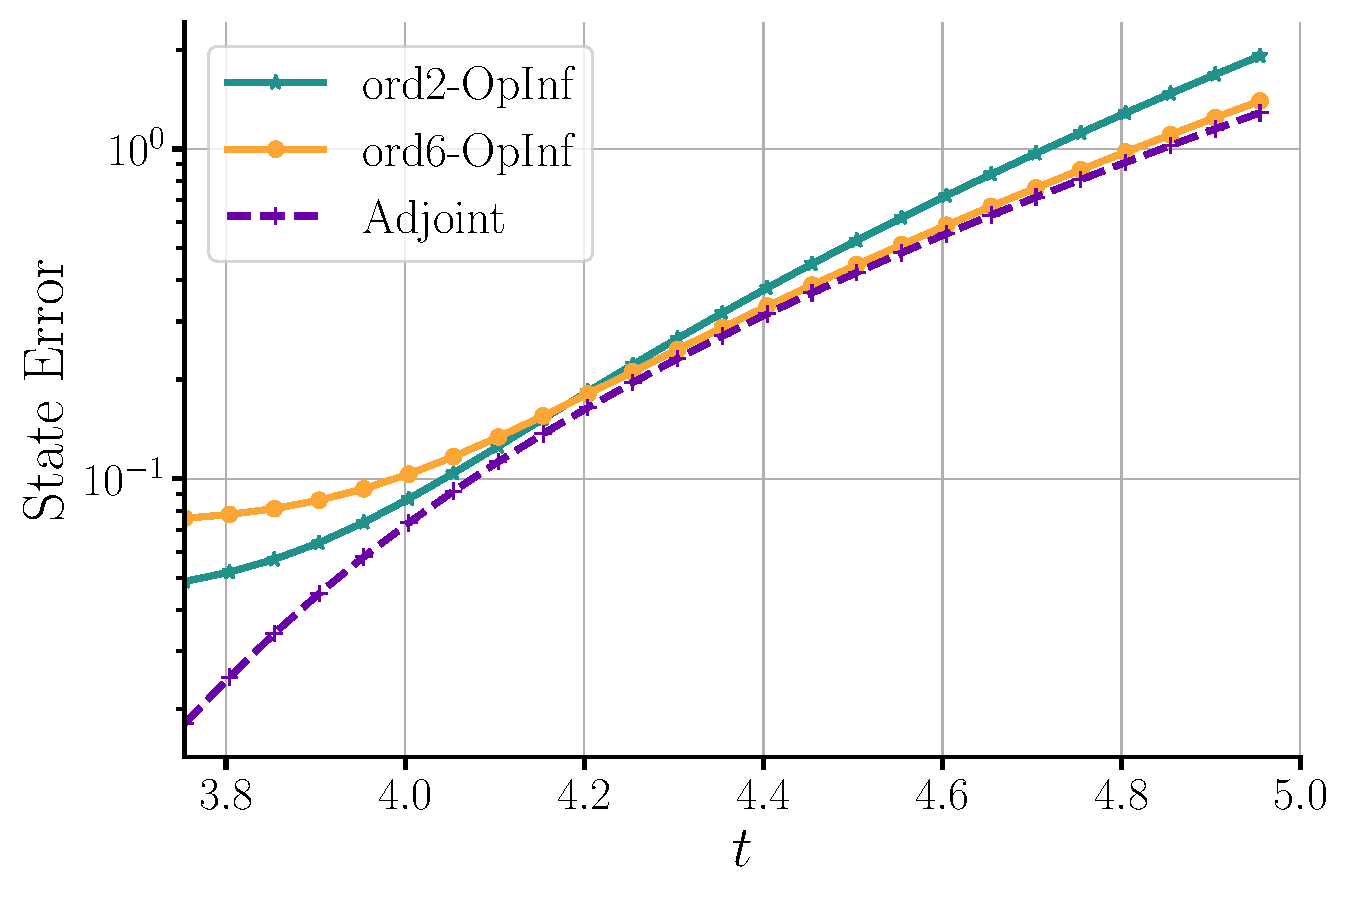
\includegraphics[width=\linewidth]{fkpp_pred_error_vs_time_noise_1.pdf}
    \caption{1\% of noise level.}
    \label{fig:image1}
  \end{subfigure}
  \quad
  \begin{subfigure}[b]{0.48\textwidth}
    \centering
    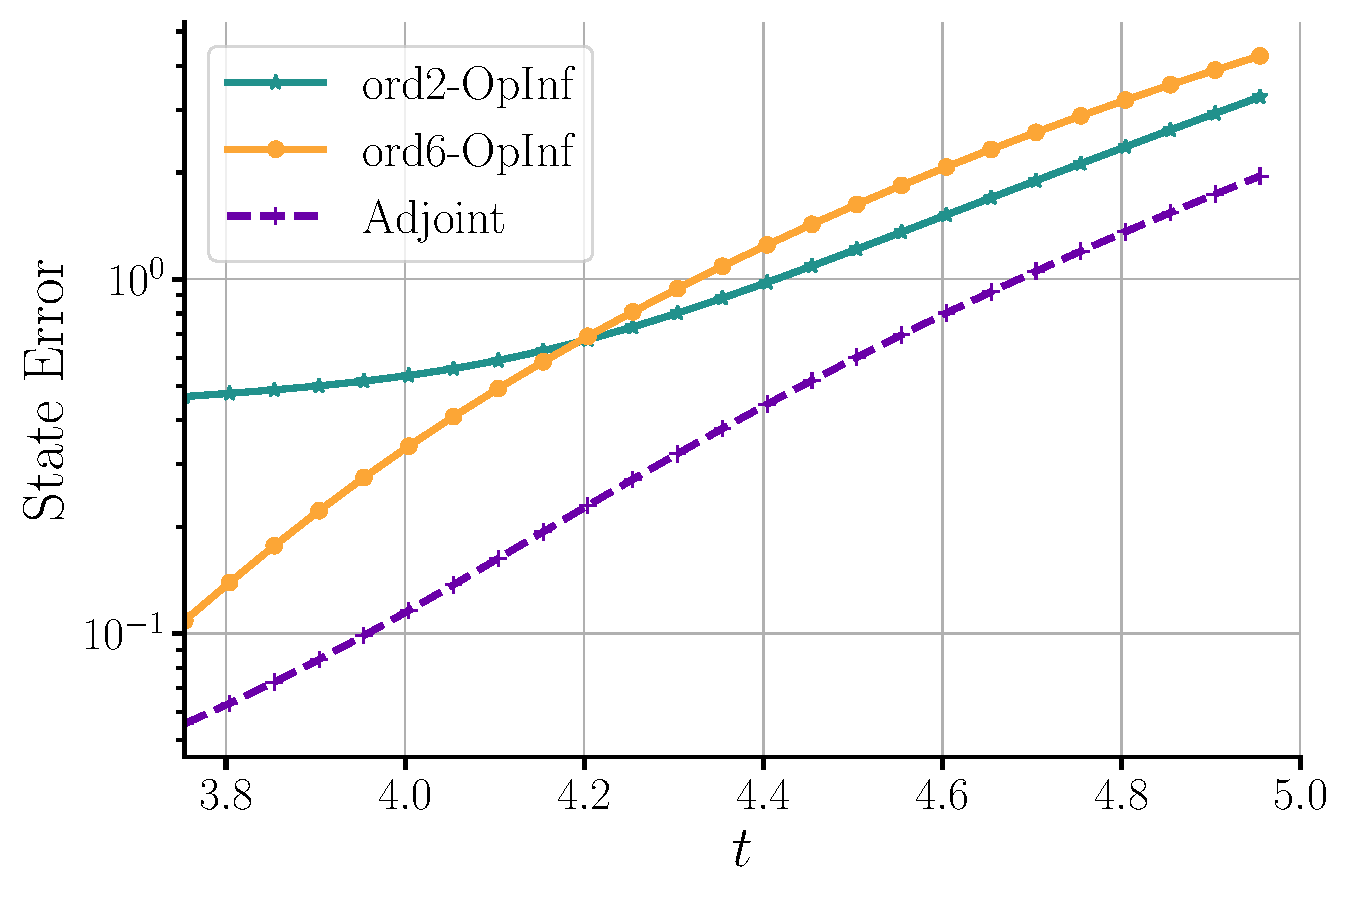
\includegraphics[width=\linewidth]{fkpp_pred_error_vs_time_noise_5.pdf}
    \caption{5\% of noise level.}
    \label{fig:image2}
  \end{subfigure}
  
  \vskip\baselineskip
  
  % Second row of subfigures
  \begin{subfigure}[b]{0.48\textwidth}
    \centering
    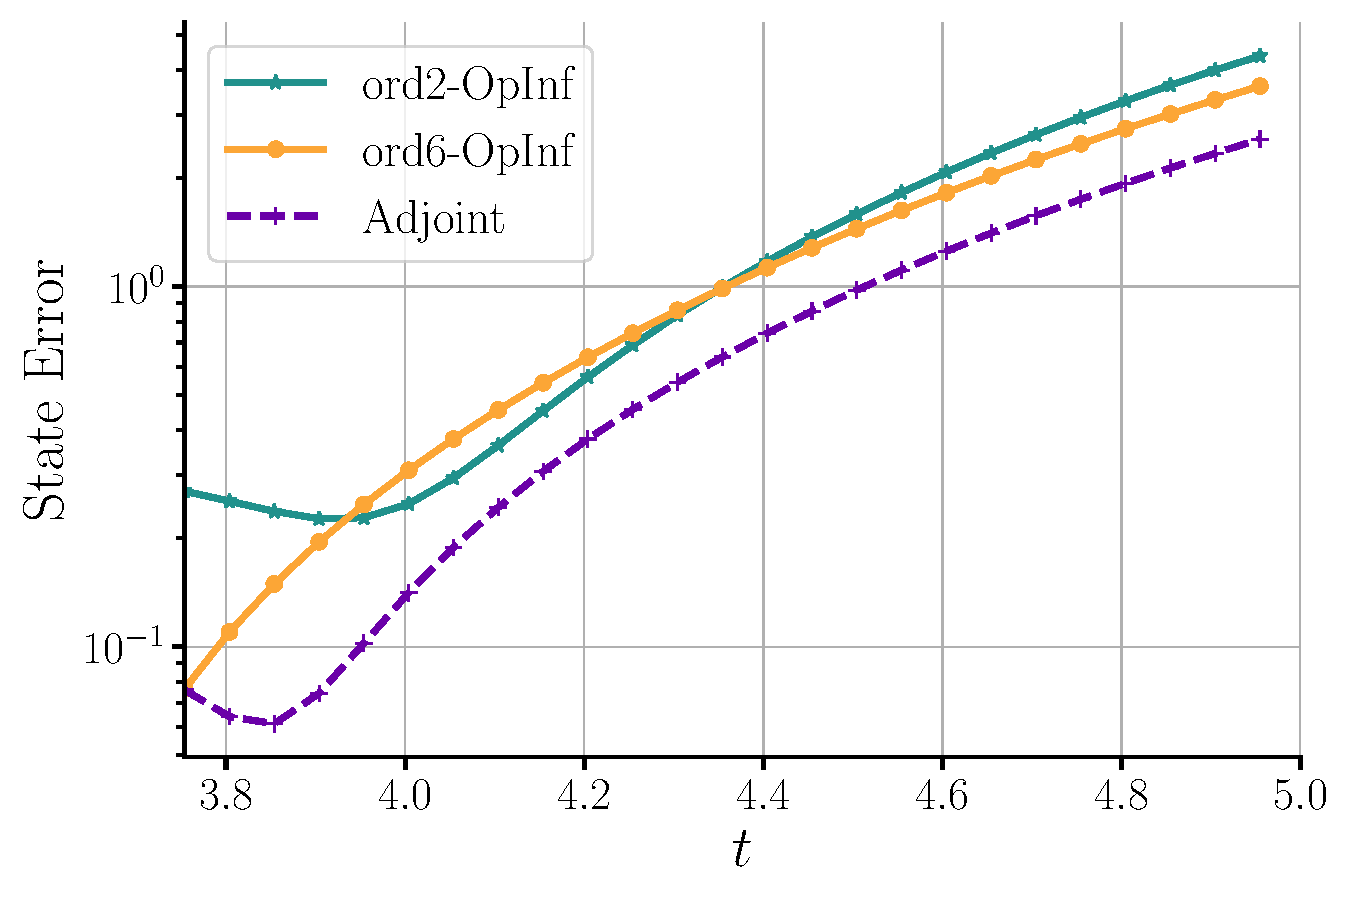
\includegraphics[width=\linewidth]{fkpp_pred_error_vs_time_noise_10.pdf}
    \caption{10\% of noise level.}
    \label{fig:image3}
  \end{subfigure}
  \quad
  \begin{subfigure}[b]{0.48\textwidth}
    \centering
    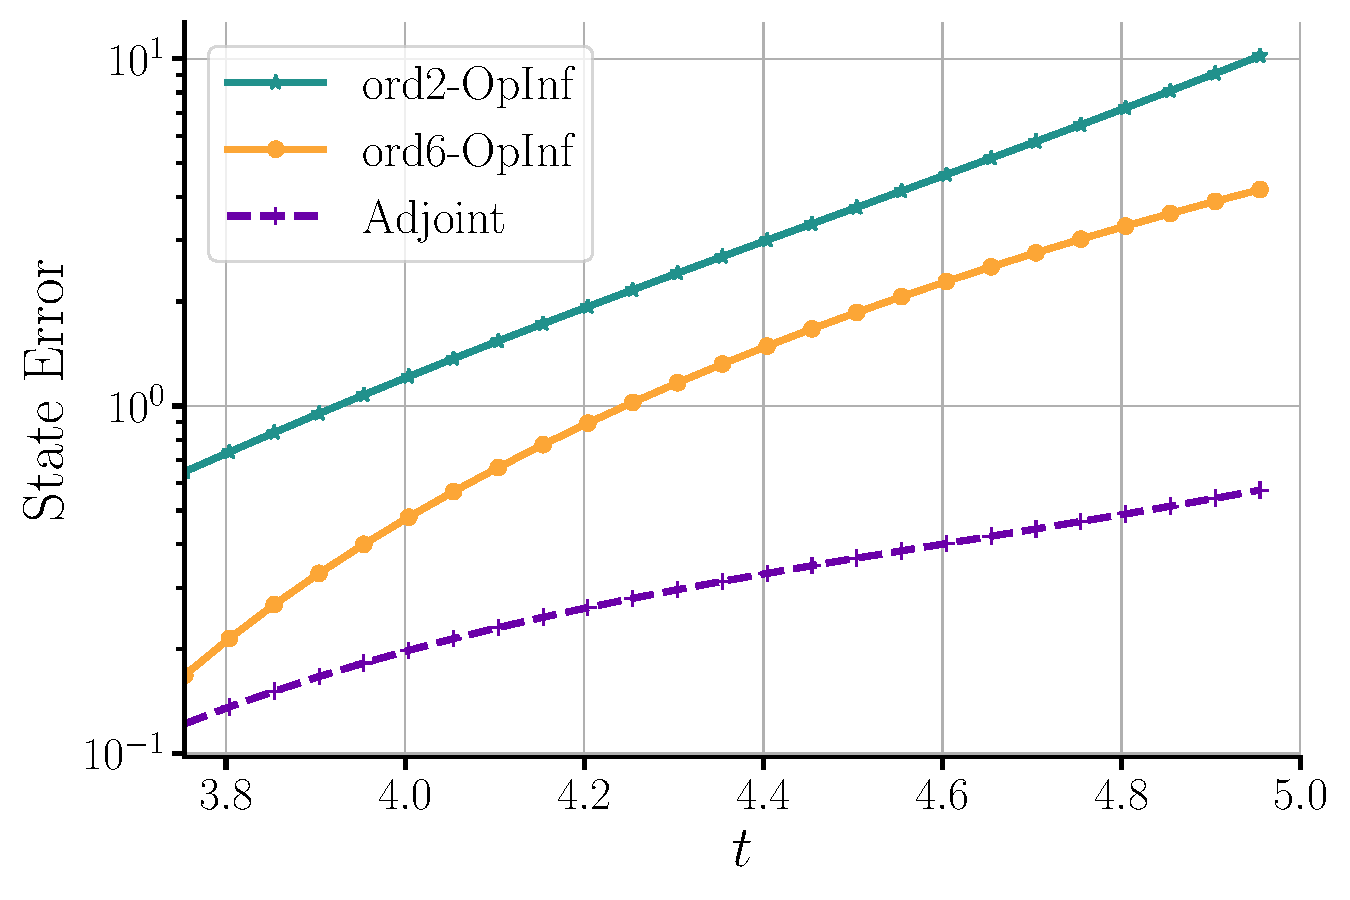
\includegraphics[width=\linewidth]{fkpp_pred_error_vs_time_noise_20.pdf}
    \caption{20\% of noise level.}
    \label{fig:image4}
  \end{subfigure}
  
  \caption{Prediction error vs. time for each noise level run in the FKPP Equation experiment.}
  \label{fig:twobytwo5}
\end{figure}

\newpage

%%%%%% Relative Error vs. r (noise - FKPP)%%%%%%

Finally, the relative error versus model dimension plots in Figure~\ref{fig:twobytwo6} demonstrate that the adjoint-trained model accuracy grows with the noise level, underscoring that exact gradient computation via this method yields more reliable parameter updates when the training snapshots are corrupted.  Overall, these findings mirror and reinforce the Burgers’ results; the adjoint method provides superior robustness to measurement noise without sacrificing computational tractability.

\vspace{0.7cm}

\begin{figure}[h!]
  \centering
  
  % First row of subfigures
  \begin{subfigure}[b]{0.48\textwidth}
    \centering
    \includegraphics[width=\linewidth]{fkpp_rel_error_vs_r_noise_1.pdf}
    \caption{1\% of noise level.}
    \label{fig:image1}
  \end{subfigure}
  \quad
  \begin{subfigure}[b]{0.48\textwidth}
    \centering
    \includegraphics[width=\linewidth]{fkpp_rel_error_vs_r_noise_5.pdf}
    \caption{5\% of noise level.}
    \label{fig:image2}
  \end{subfigure}
  
  \vskip\baselineskip
  
  % Second row of subfigures
  \begin{subfigure}[b]{0.48\textwidth}
    \centering
    \includegraphics[width=\linewidth]{fkpp_rel_error_vs_r_noise_10.pdf}
    \caption{10\% of noise level.}
    \label{fig:image3}
  \end{subfigure}
  \quad
  \begin{subfigure}[b]{0.48\textwidth}
    \centering
    \includegraphics[width=\linewidth]{fkpp_rel_error_vs_r_noise_20.pdf}
    \caption{20\% of noise level.}
    \label{fig:image4}
  \end{subfigure}
  
  \caption{Relative error vs. $r$ for each noise perturbation run in the FKPP Equation experiment.}
  \label{fig:twobytwo6}
\end{figure}

\newpage

%%%%%%%%%%%%%%%%%%%%%%%%%%%%%%%%%%%%%%%%%%%%%%%%%%%%%%%%%%%%%%%%%%%%%%%%%%%%%%%%%%%%%%%